\chapter{Supplements PixArt-$\Sigma$ Experiments}

\section{Experimental Default Setup}
\begin{table}[H]
	\centering
	\caption[PixArt-$\Sigma$ Fine-Funing Hyperparameters]{Default hyperparameter settings for PixArt-$\Sigma$ fine-tuning after compression.}
	\label{tab:hyperparameterTraining}
	\begin{tabular}{l c}
		\toprule
		\textbf{Hyperparameter} & \textbf{Value} \\
		\midrule
		\multicolumn{2}{l}{\textit{\textbf{Optimization}}} \\
		\midrule
		Optimizer Type & CAME \\
		Learning Rate & $2 \times 10^{-5}$ (Block Removal)/ $2 \times 10^{-6}$ (SVD Compression)\\
		Weight Decay & $0.03$ \\
		Betas & $(0.9, 0.999, 0.9999)$ \\
		Epsilon & $(10^{-30}, 10^{-16})$ \\
		\midrule
		\multicolumn{2}{l}{\textit{\textbf{Training Schedule}}} \\
		\midrule
		Warmup Steps & 1000 \\
		Batch Size & 16 \\
		Gradient Clipping & $0.001$ \\
		\midrule
		\multicolumn{2}{l}{\textit{\textbf{Model \& Data}}} \\
		\midrule
		Precision & bf16 \\
		Resolution & $512 \times 512$ \\
		Class Dropout Prob. & $0.1$ \\
		Max Prompt Length & 300 \\
		\bottomrule
	\end{tabular}
\end{table}

\section{Block Importance Analysis}
This appendix provides a \gls{CKA}-score analysis across all PixArt-$\Sigma$ blocks and across all timesteps. It demonstrates that the \gls{CKA}-score can vary significantly for one block over the course of the image generation trajectory (e.g., block 22), indicating that blocks have different importance at different timesteps (Fig. \ref{fig:PixArtBlockImportanceHeatmap}). Furthermore, it provides all images for the qualitative analysis of block compression by 60\% (Fig. \ref{fig:AppxPixArtCMMDCompression})

\subsubsection{CKA-Analysis of Transformer Blocks}

\begin{figure}[H]
	\centering
	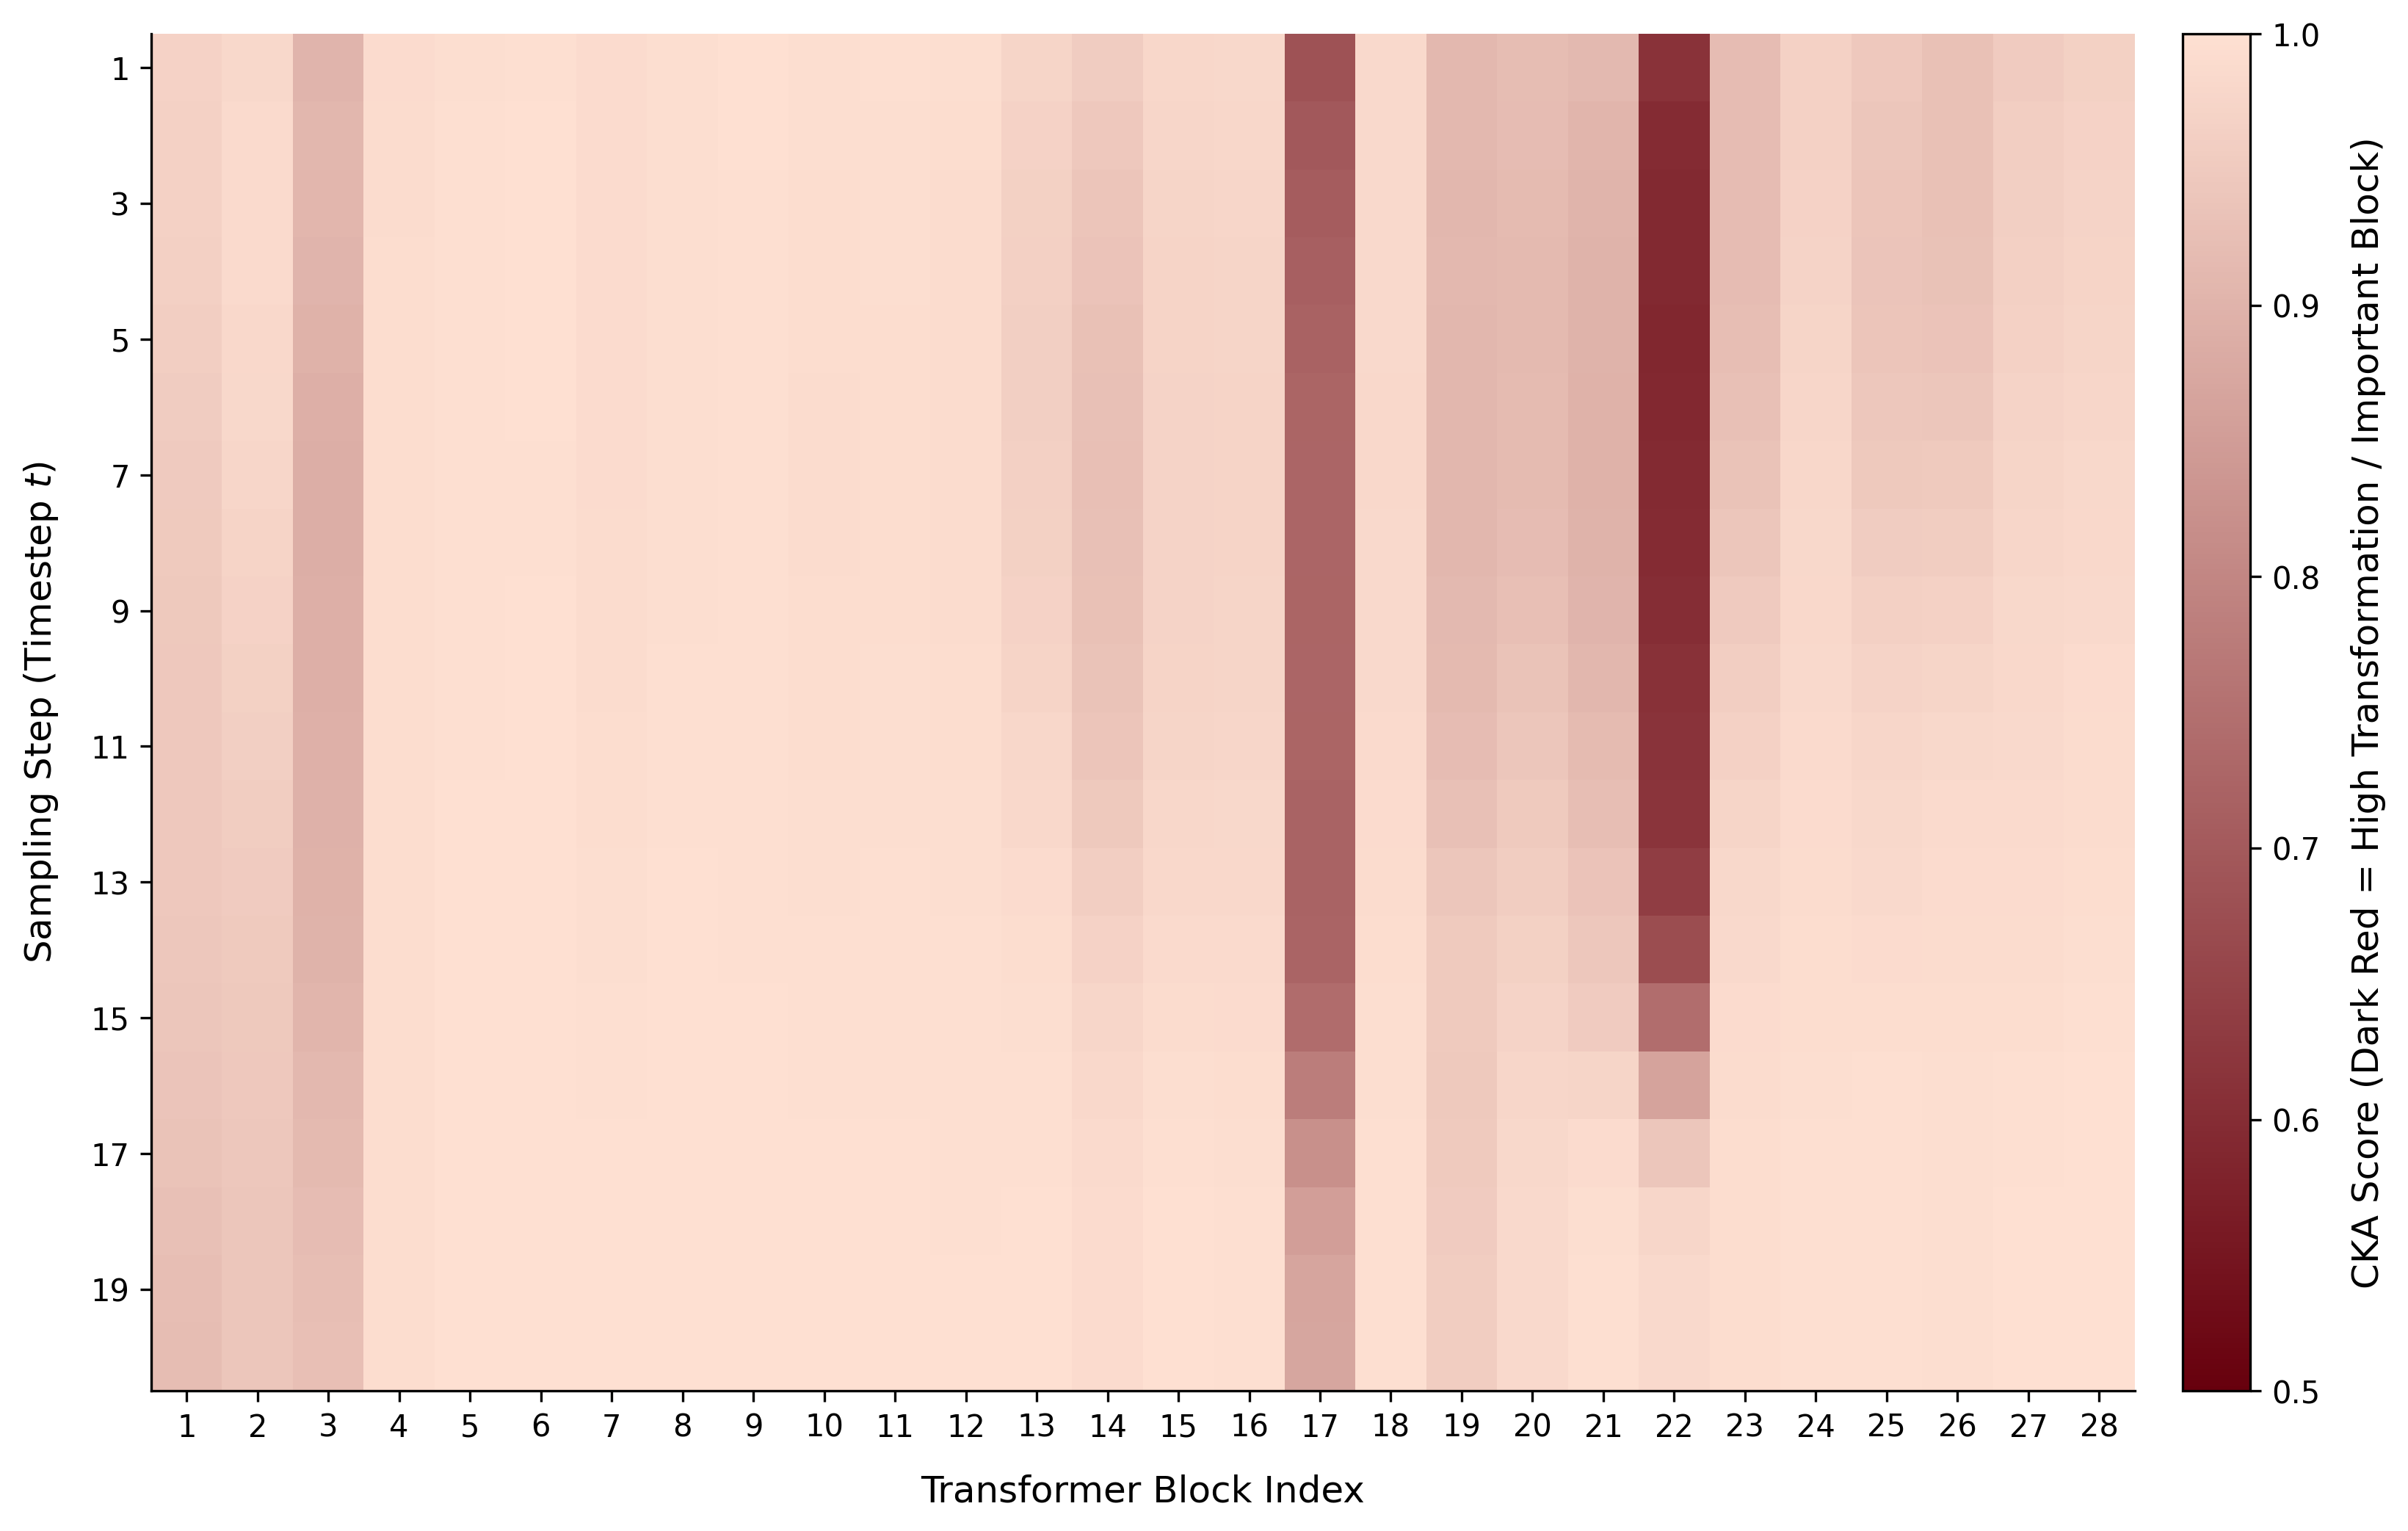
\includegraphics[width=0.65\textwidth]{images/Experimente/Pixart_Block_Analysis/cka_heatmap_100_thesis.png}  % adjust filename and width
	\caption[CKA-Score Heatmap]{The heatmap displays the \gls{CKA} score for all PixArt-$\Sigma$ blocks across all timesteps.}
	
	\label{fig:PixArtBlockImportanceHeatmap}
\end{figure}

\subsubsection{Qualitative Block Selection Analysis}
\begin{figure}[H]
	\centering
	
\includegraphics[width=0.7\textwidth]{images/Experimente/PixArt_Block_Analysis/BlockAnalysisCompression06.pdf}  % adjust filename and width
	\caption[Qualitative Block Importance Analysis of PixArt-$\Sigma$: Block Compression]{Illustration of the impact of selectively compressing individual Transformer blocks (1–28) by 60\% on the final generation result.}
	
	\label{fig:AppxPixArtCMMDCompression}
\end{figure}




\section{One-Shot vs. Progressive Pruning}
\label{sec:OneShotVsProgressivePrunAppendix}
Tab. \ref{tab:SettingOneShotvsProgressive} provides information of the technical settings of the experiments for the comparison of one-shot vs. progressive model pruning.
Moreover, this section presents qualitative example images generated by models compressed to various ratios (Figs. \ref{fig:FinetuningProtocol_Appx90} - \ref{fig:FinetuningProtocol_60}). These were obtained using the one-shot and progressive pruning approaches, as detailed in Section \ref{sec:OneShot_vs_Progressive_Pruning}. Note that for the model pruned to 90\%, the one-shot and progressive pruning schedules are identical.


\begin{table}[H]
	\centering
\caption[Block Removal Details: One-Shot vs. Progressive Pruning]{Overview of the compression details utilized for the one-shot and progressive pruning experiments on the PixArt-$\Sigma$ model.}
	\label{tab:SettingOneShotvsProgressive}
	\begin{tabular}{@{} l c c c @{}}
		\toprule
		\textbf{Model Variant} & \textbf{Number of}  & \textbf{Training Steps} \\
		\textbf{(Remaining \%)} & \textbf{Removed Blocks}  & \textbf{(in Thousands)} \\
		\midrule
		Model 90\% & 3 & 88.5 \\
		Model 80\% & 6   & 265.5 \\
		Model 70\% & 8   & 531.0 \\
		Model 60\% & 11  & 708.0 \\
		Model 50\% & 14  & 973.5 \\
		\bottomrule
	\end{tabular}
	
\end{table}




\begin{figure}[H]
	\centering
	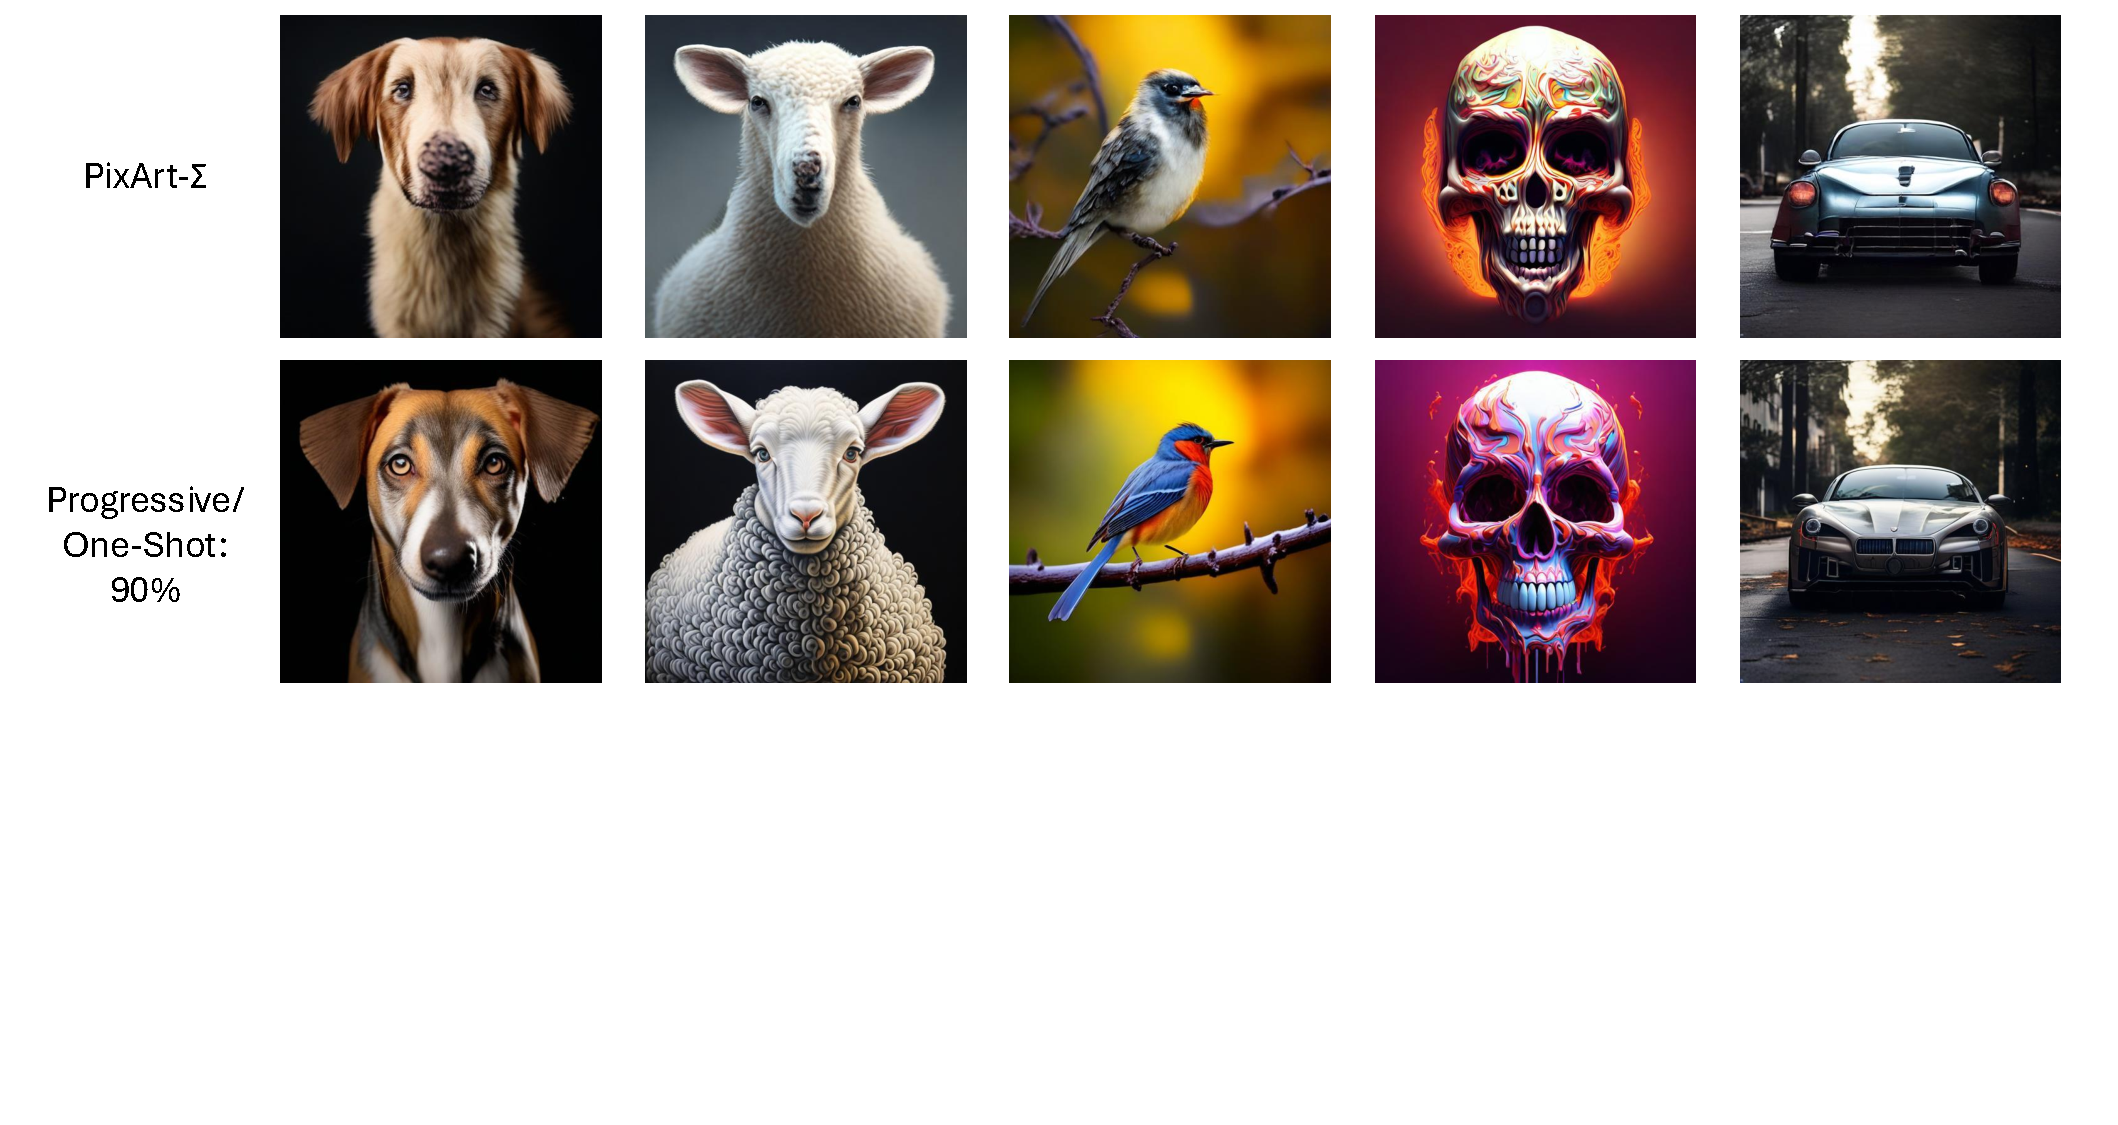
\includegraphics[width=0.7\textwidth]{images/Experimente/Iterative_vs_Direct/Examples_model_90.pdf}
	\caption[Qualitative Examples: One-Shot vs. Progressive Model Pruning (90\% Pruning)]{Qualitative comparison of example images generated by models pruned to 90\% using either a one-shot or a progressive pruning strategy.}
	\label{fig:FinetuningProtocol_Appx90}
\end{figure}


\begin{figure}[H]
	\centering
	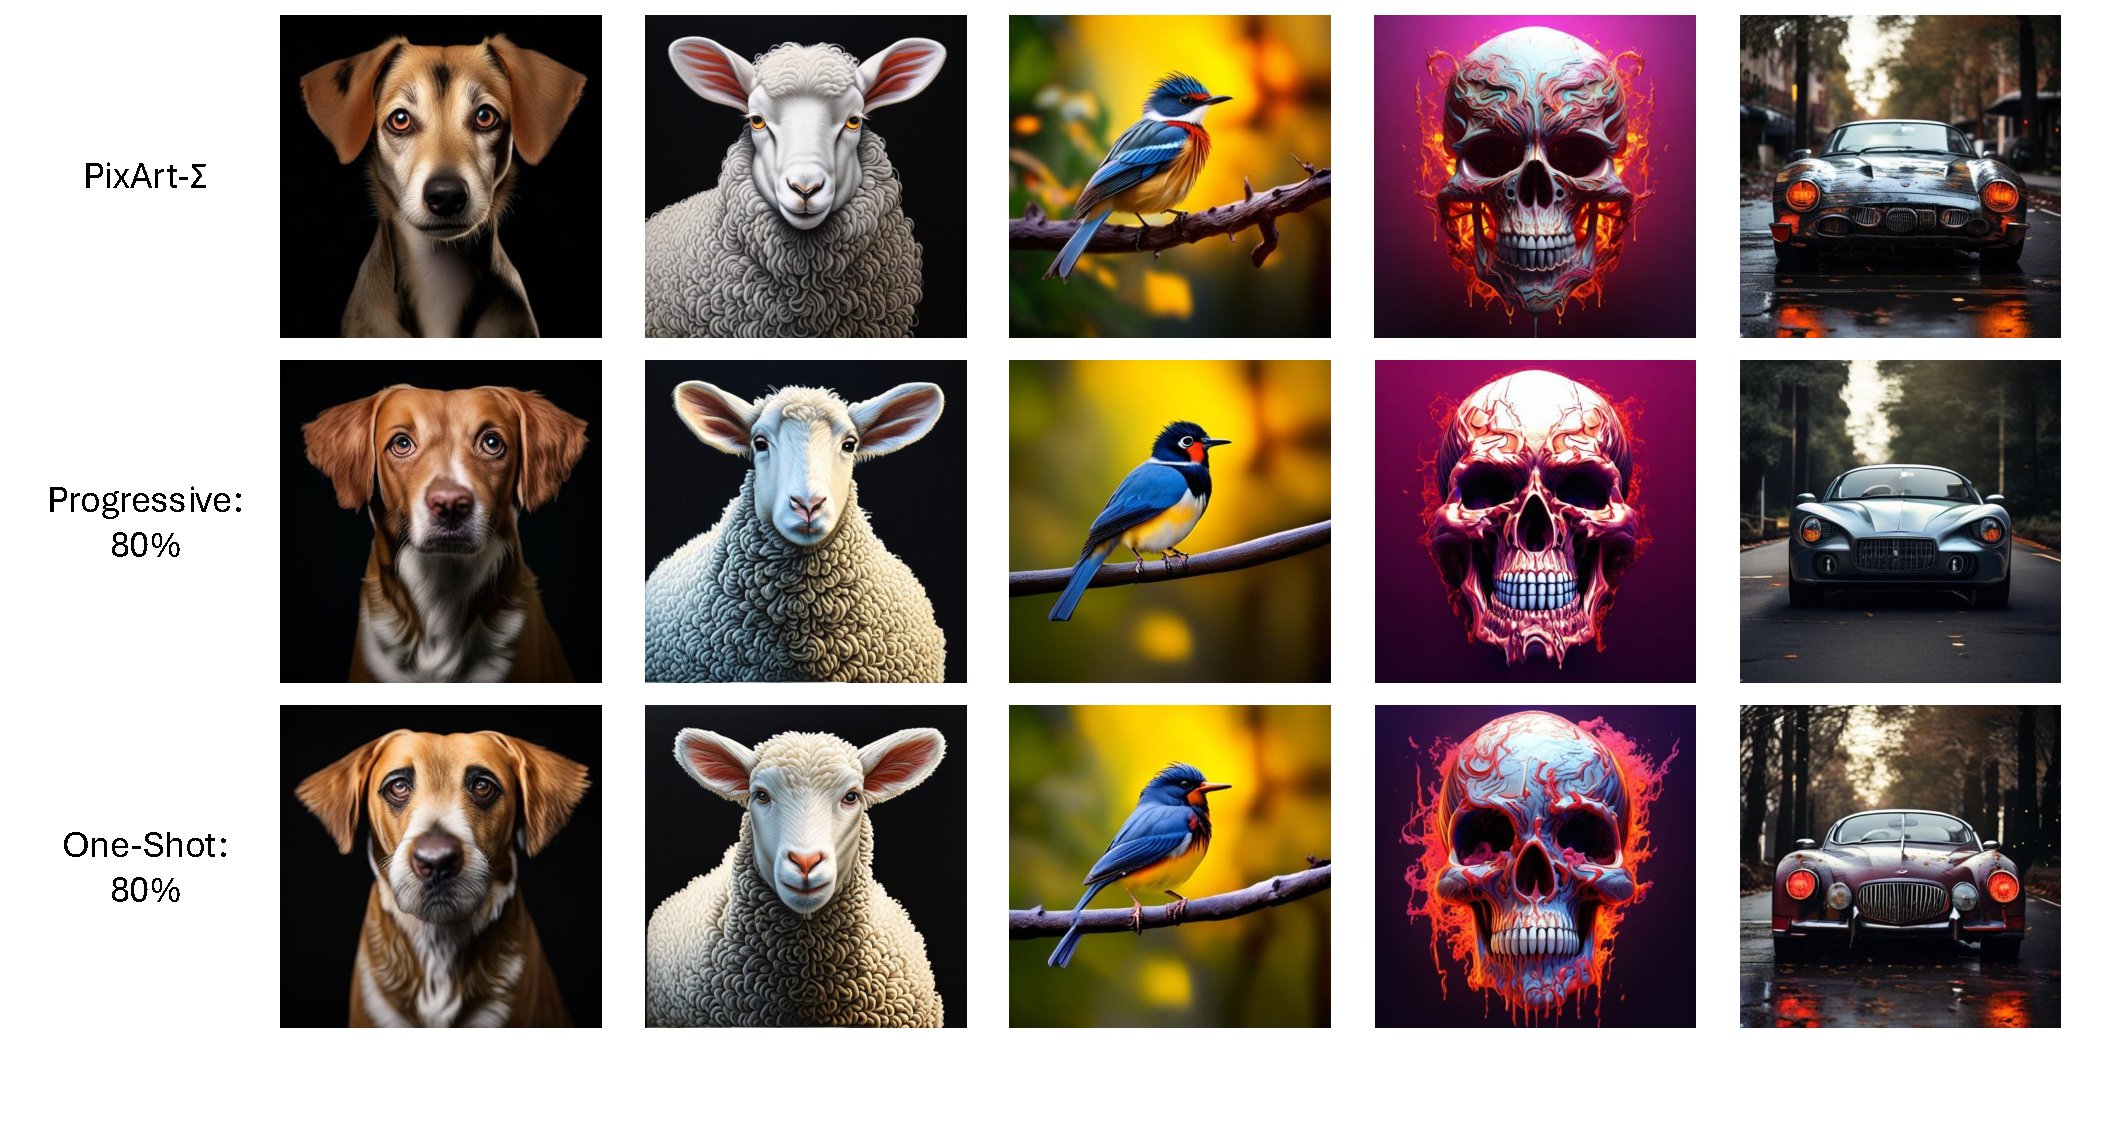
\includegraphics[width=0.7\textwidth]{images/Experimente/Iterative_vs_Direct/Examples_model_80.pdf}
	\caption[Qualitative Examples: One-Shot vs. Progressive Model Pruning (80\% Pruning)]{Qualitative comparison of example images generated by models pruned to 80\% using either a one-shot or a progressive pruning strategy.}
	\label{fig:FinetuningProtocol_Appx80}
\end{figure}

\begin{figure}[H]
	\centering
	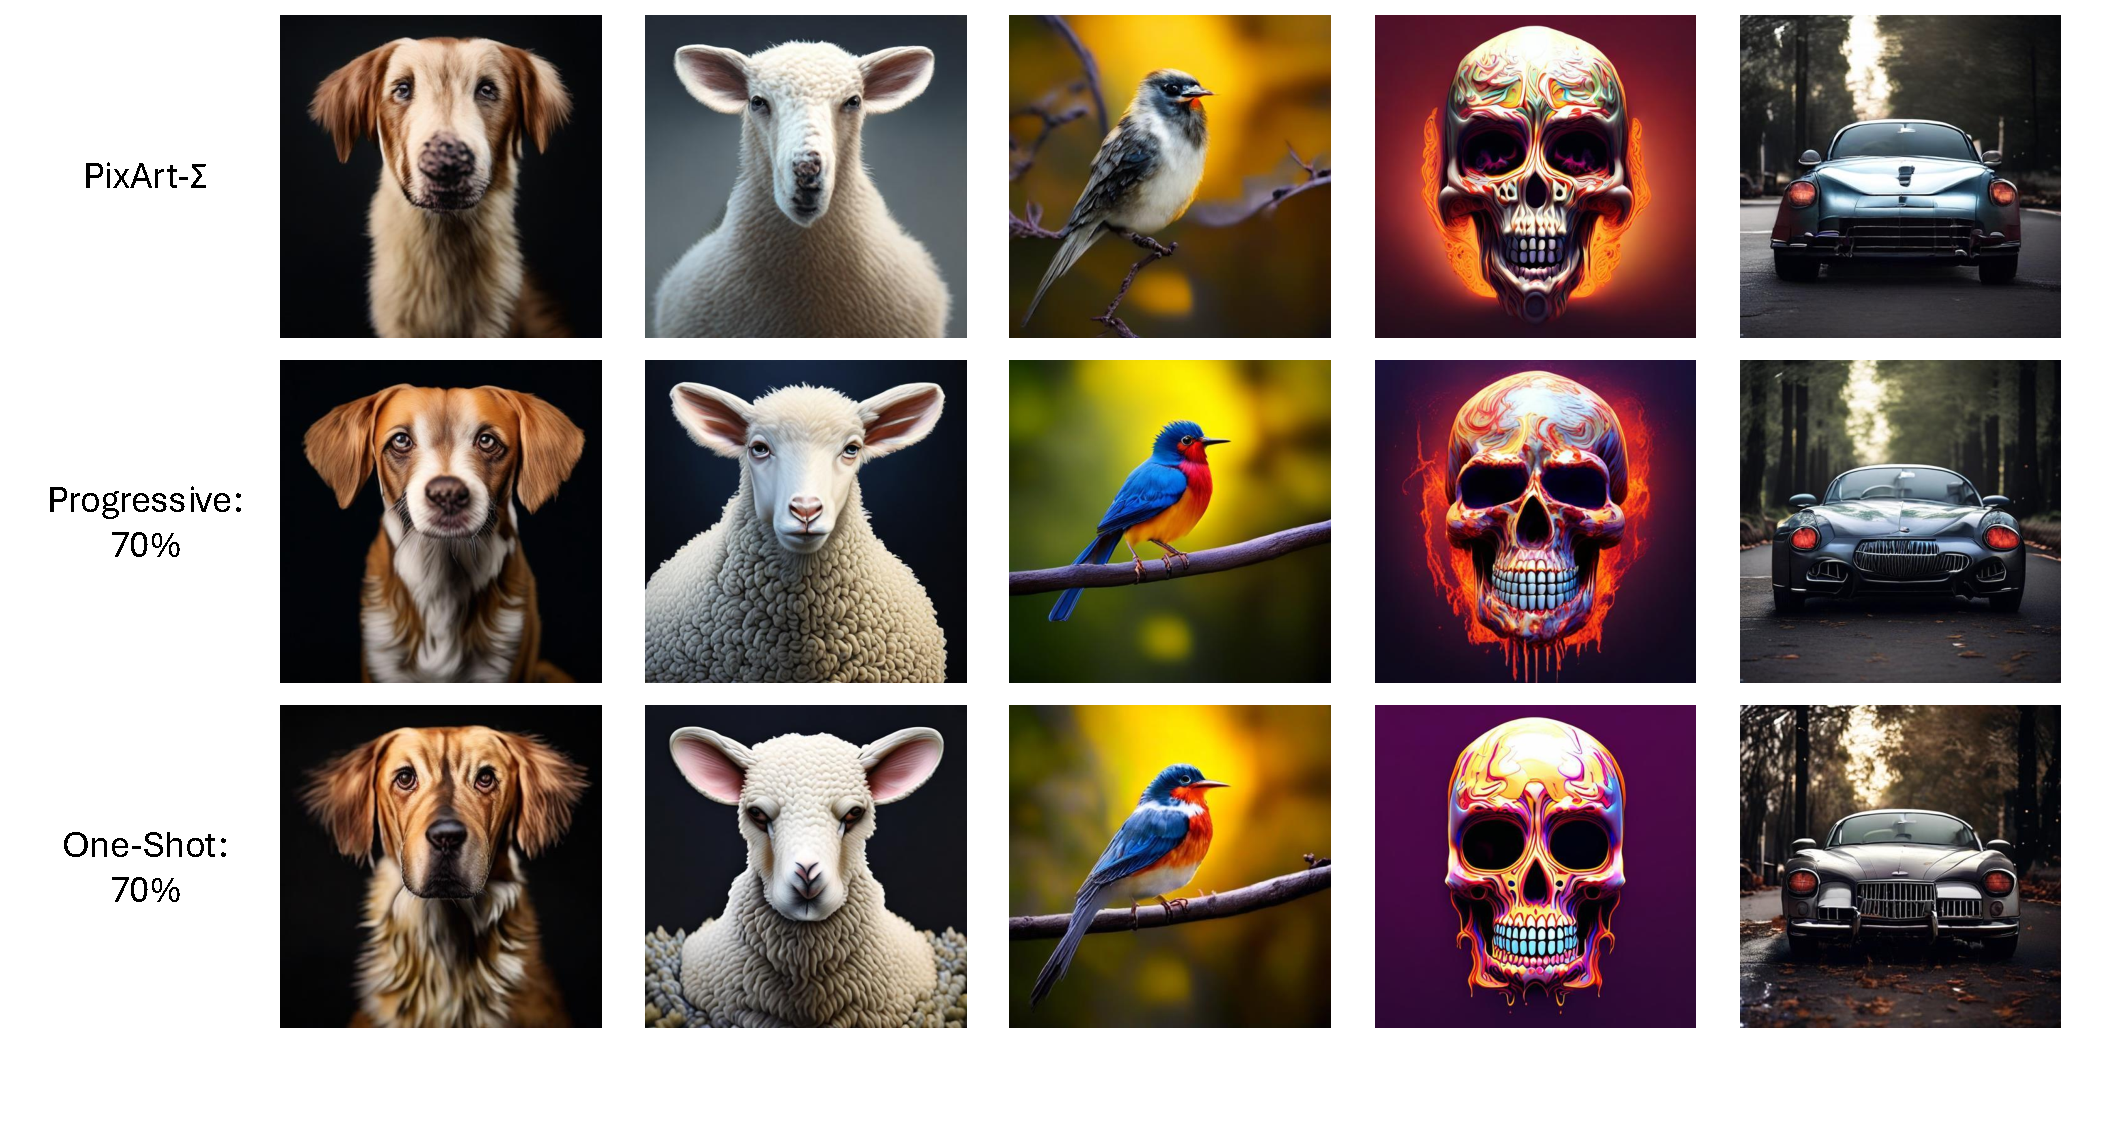
\includegraphics[width=0.7\textwidth]{images/Experimente/Iterative_vs_Direct/Examples_model_70.pdf}
	\caption[Qualitative Examples: One-Shot vs. Progressive Model Pruning (70\% Pruning)]{Qualitative comparison of example images generated by models pruned to 70\% using either a one-shot or a progressive pruning strategy.}
	\label{fig:FinetuningProtocol_70}
\end{figure}

\begin{figure}[H]
	\centering
	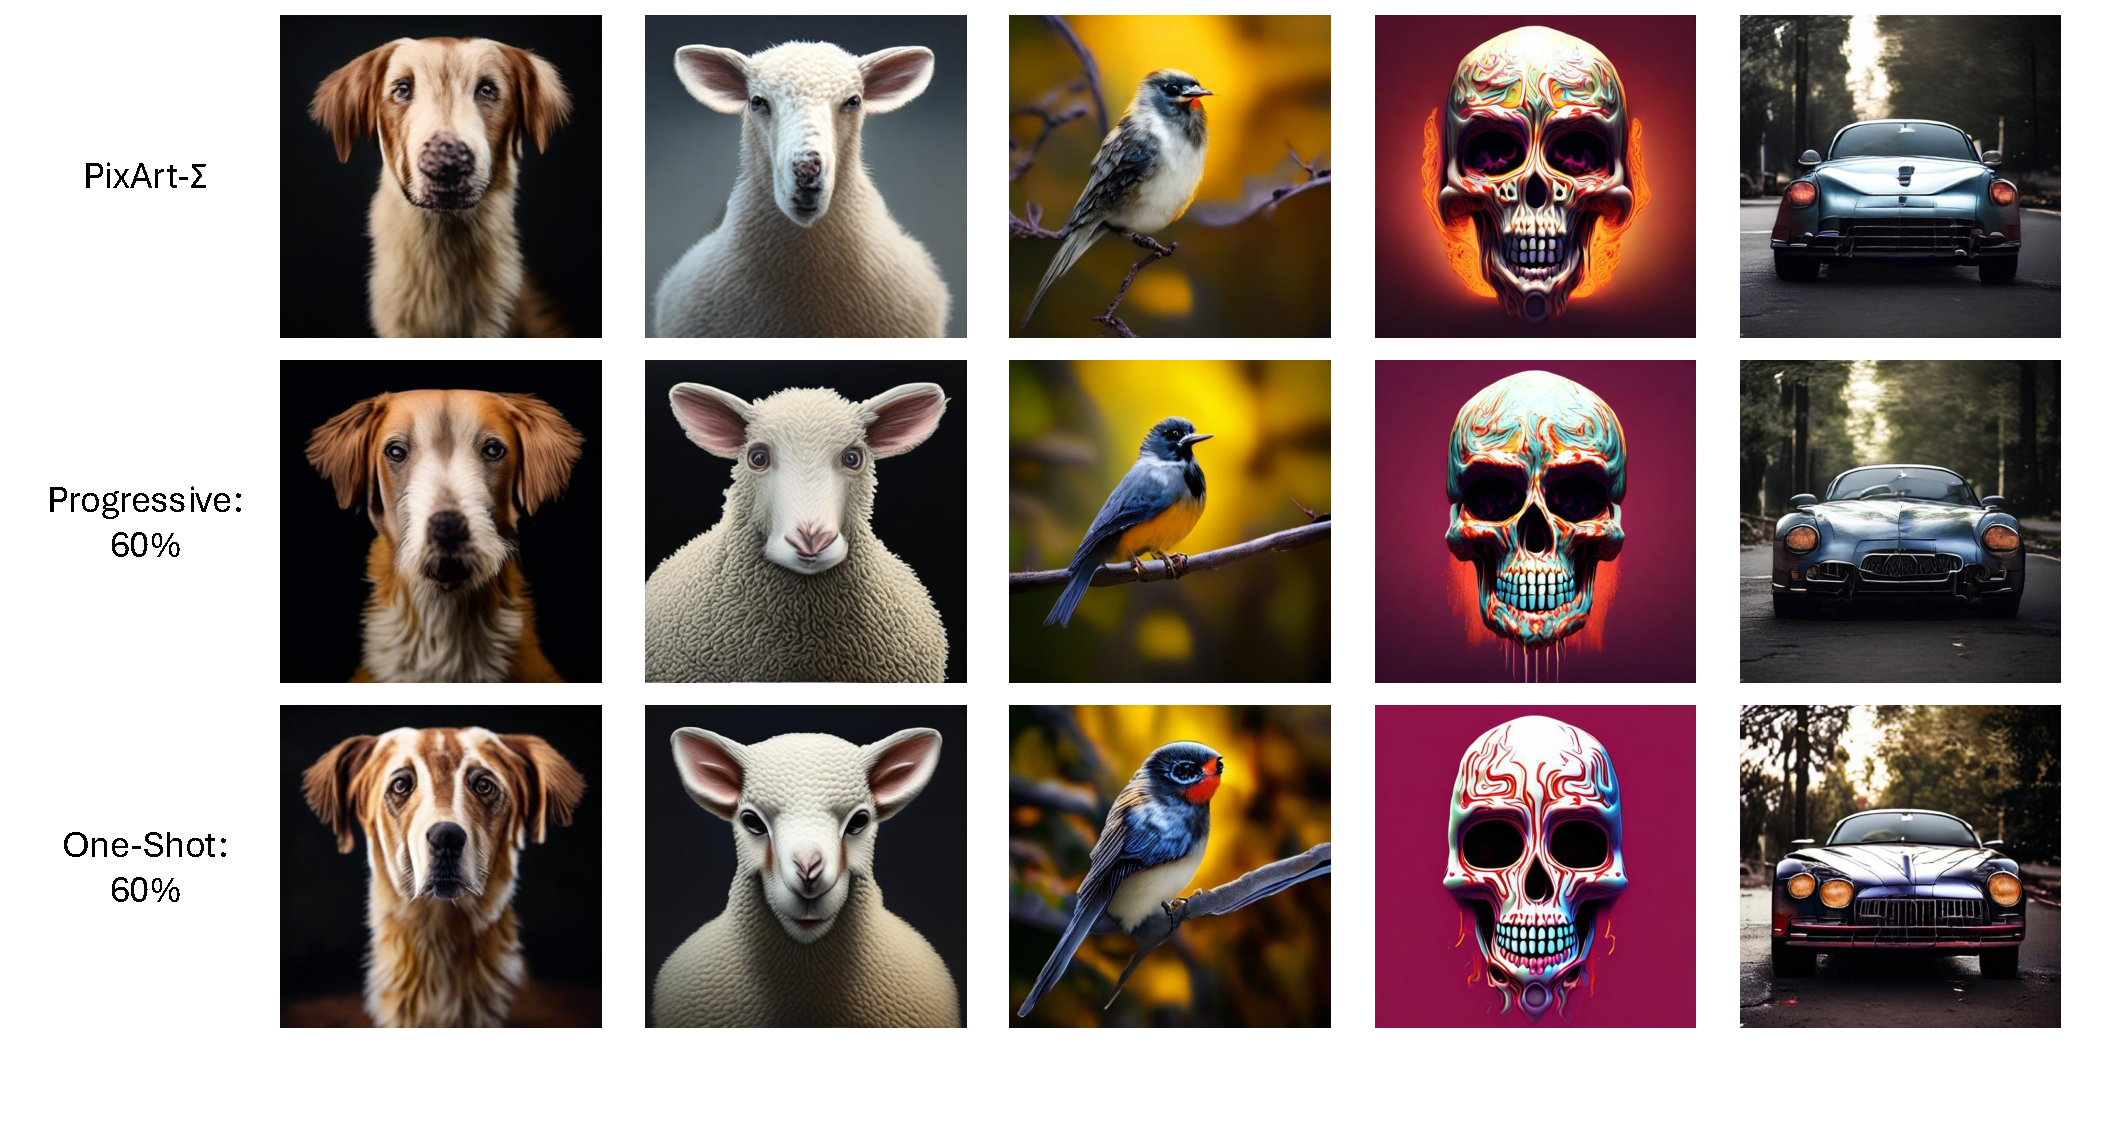
\includegraphics[width=0.7\textwidth]{images/Experimente/Iterative_vs_Direct/Examples_model_60.pdf}
	\caption[Qualitative Examples: One-Shot vs. Progressive Model Pruning (60\% Pruning)]{Qualitative comparison of example images generated by models pruned to 60\% using either a one-shot or a progressive pruning strategy.}
	\label{fig:FinetuningProtocol_60}
\end{figure}

\section{Knowledge Distillation Loss}
\label{sec:KnowledgeDistillationAppendix}
This section provides an analysis of the average feature magnitudes across individual PixArt-$\Sigma$ transformer blocks, measured via the \gls{RMS} norm (Fig. \ref{fig:MagnitudeIntermediateFeatures}). Furthermore, it includes qualitative examples comparing various knowledge distillation loss configurations across several model compression ratios (Fig. \ref{fig:QualitativeLossInvestigation_90} - \ref{fig:QualitativeLossInvestigation_50}).

  \begin{figure}[H]
	\centering
	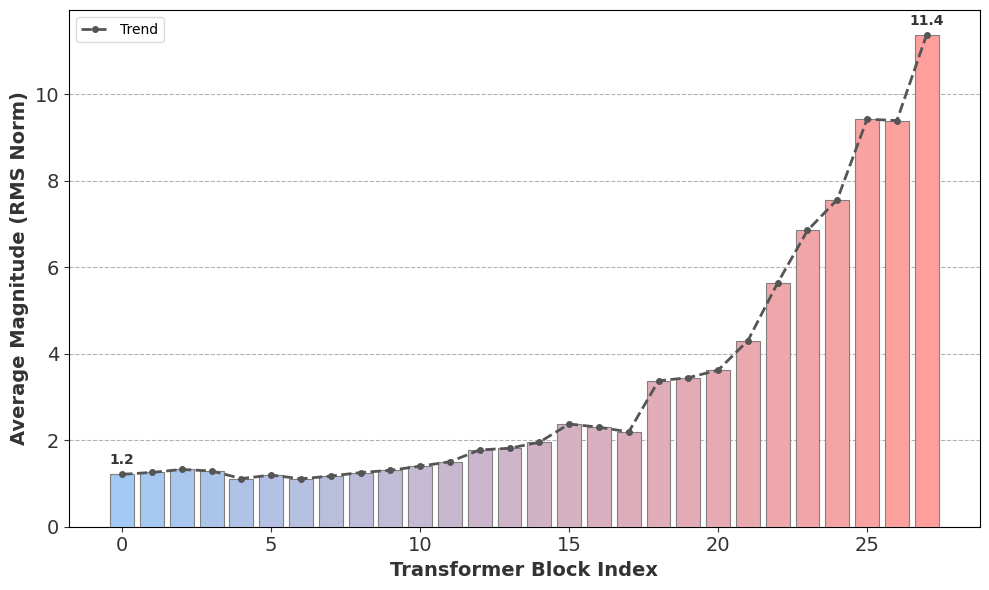
\includegraphics[width=0.6\textwidth]{images/Experimente/loss_investigation/magnitude_block_features.png}  
\caption[Magnitude of Intermediate Features in PixArt-$\Sigma$]{The \gls{RMS} norm of output features across individual PixArt-$\Sigma$ transformer blocks exhibits significant variance, with later layers generally displaying larger magnitudes than preceding ones. Results are averaged over 100 prompts from the LAION dataset.}
	\label{fig:MagnitudeIntermediateFeatures}
\end{figure}


\begin{figure}[H]
	\centering
	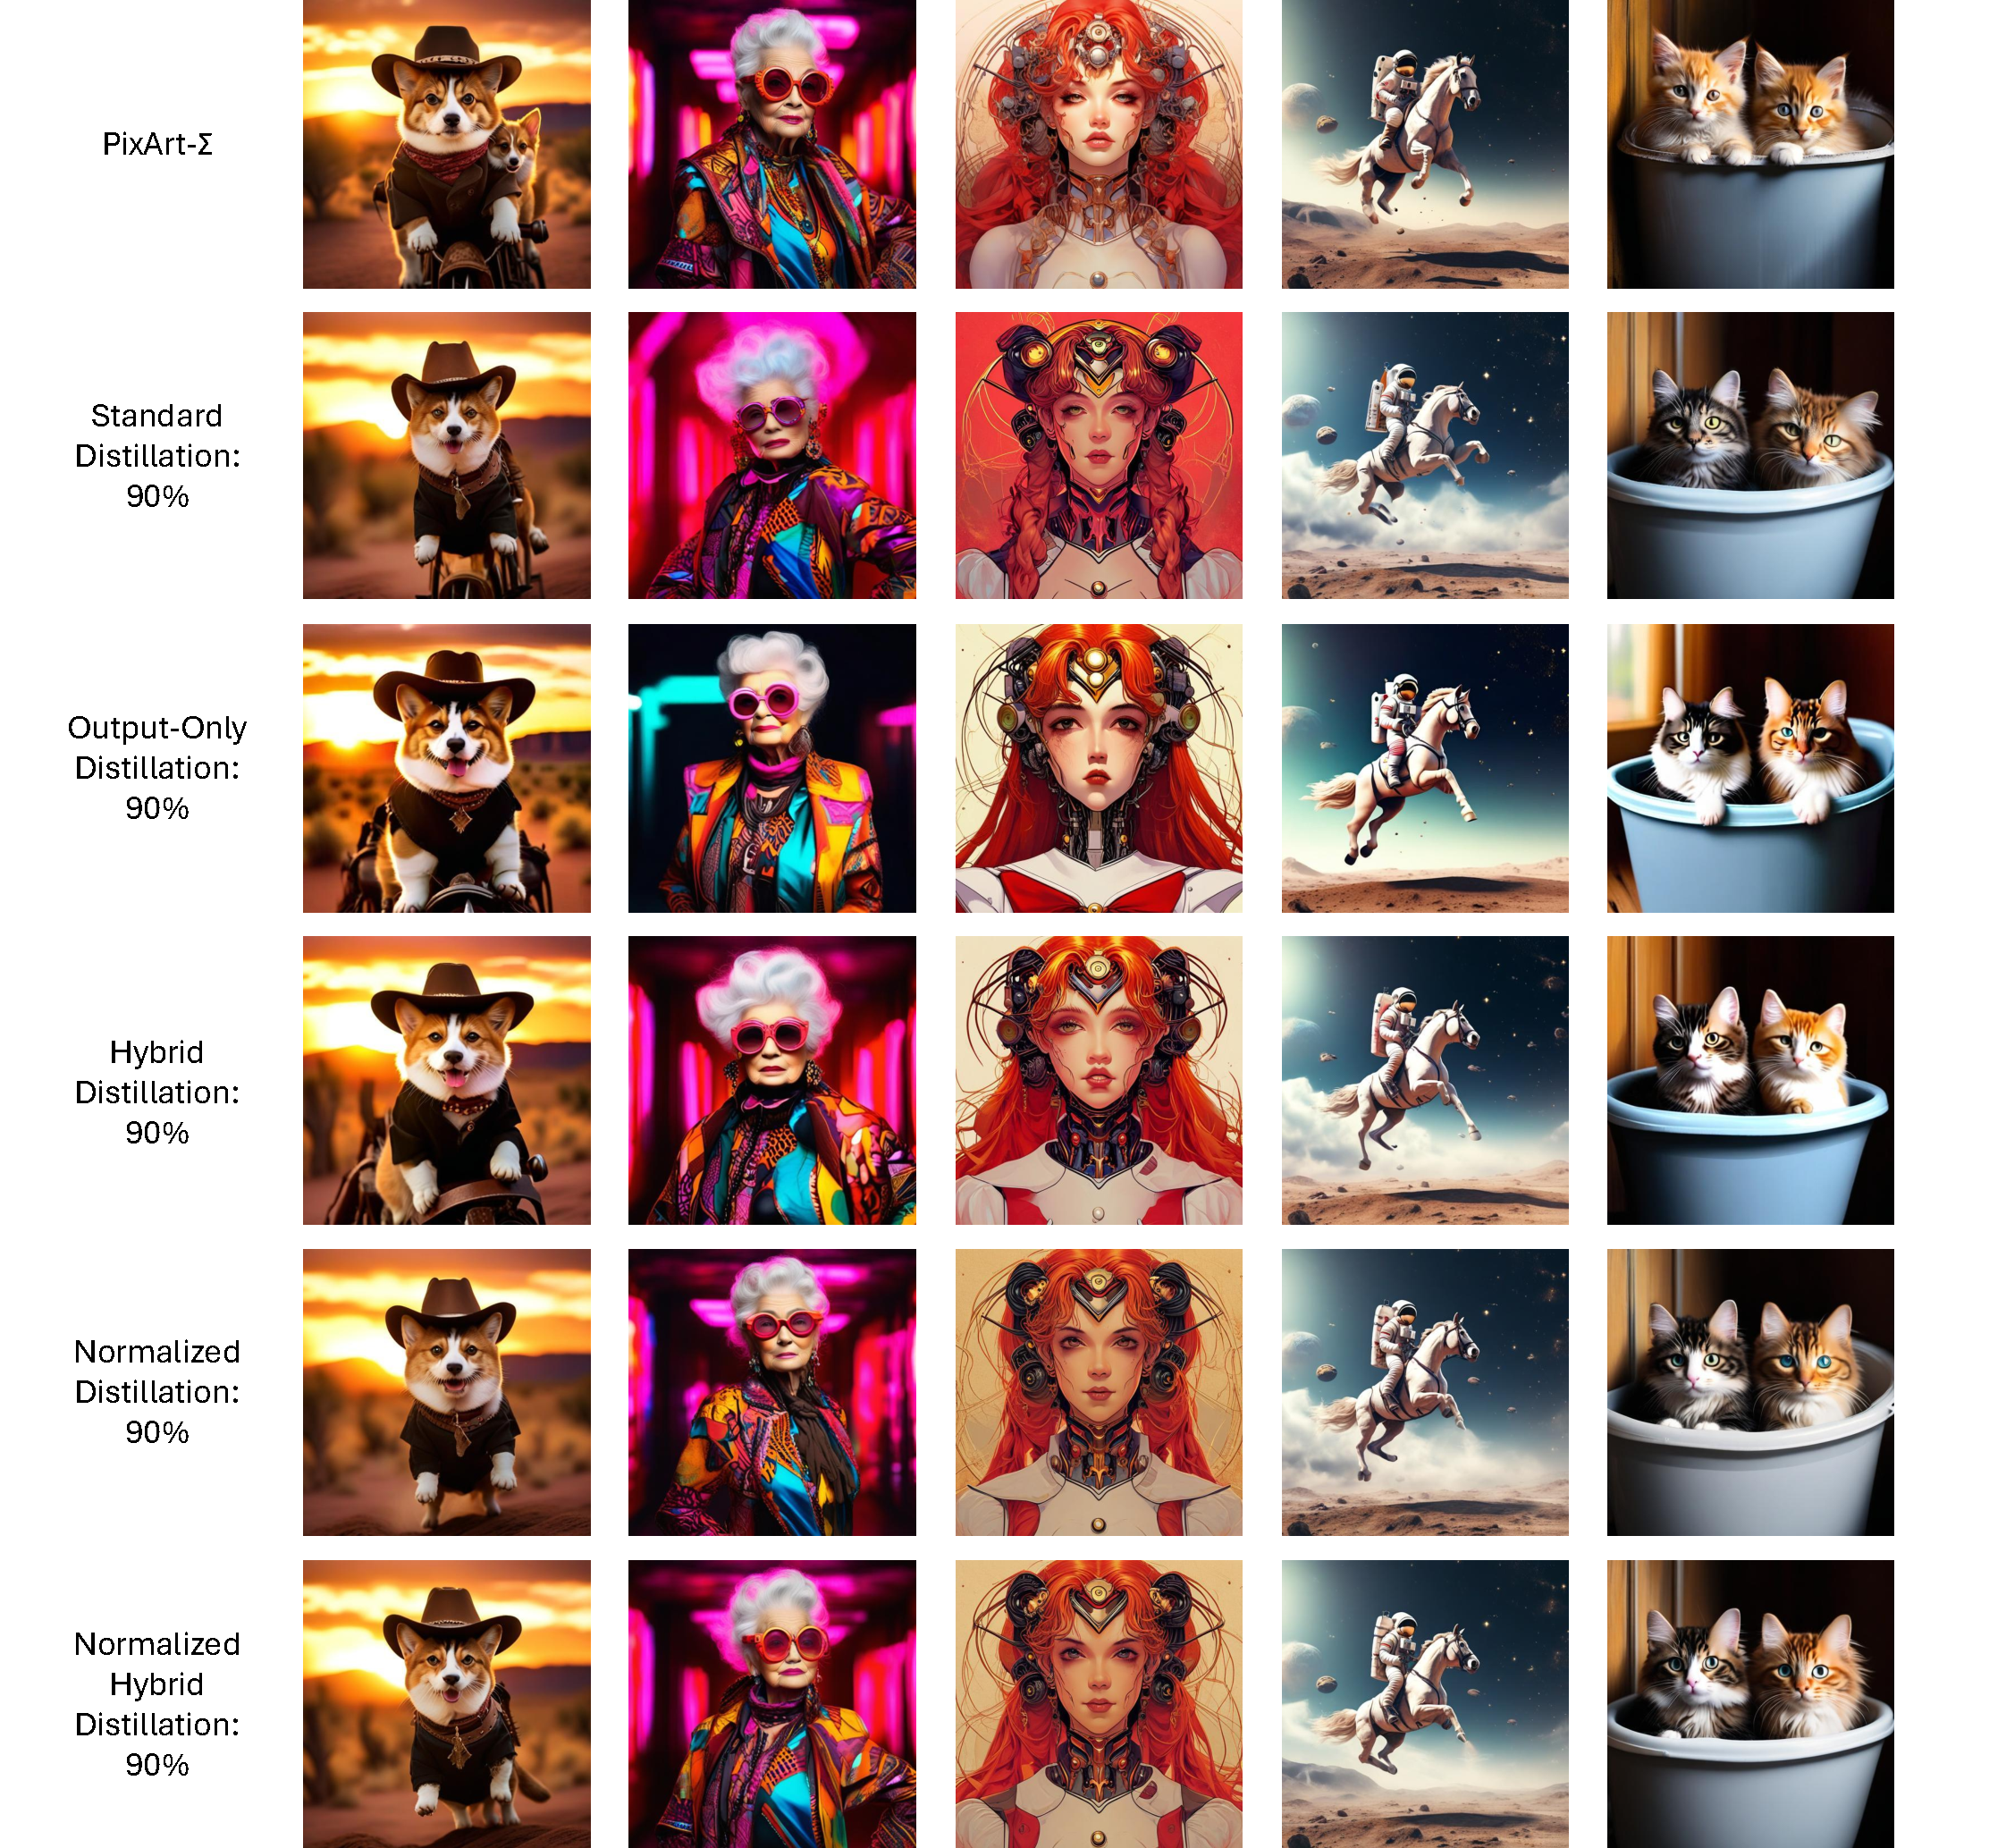
\includegraphics[width=0.65\textwidth]{images/Appendix/KnowledgeDistillation/model_90.pdf}
 	\caption[Qualitative Examples: Different Knowledge Distillation Loss Configurations (90\% Pruning)]{Qualitative comparison of example images generated by models pruned to 90\% using various knowledge distillation loss configurations}
	\label{fig:QualitativeLossInvestigation_90}
\end{figure}

\begin{figure}[H]
	\centering
	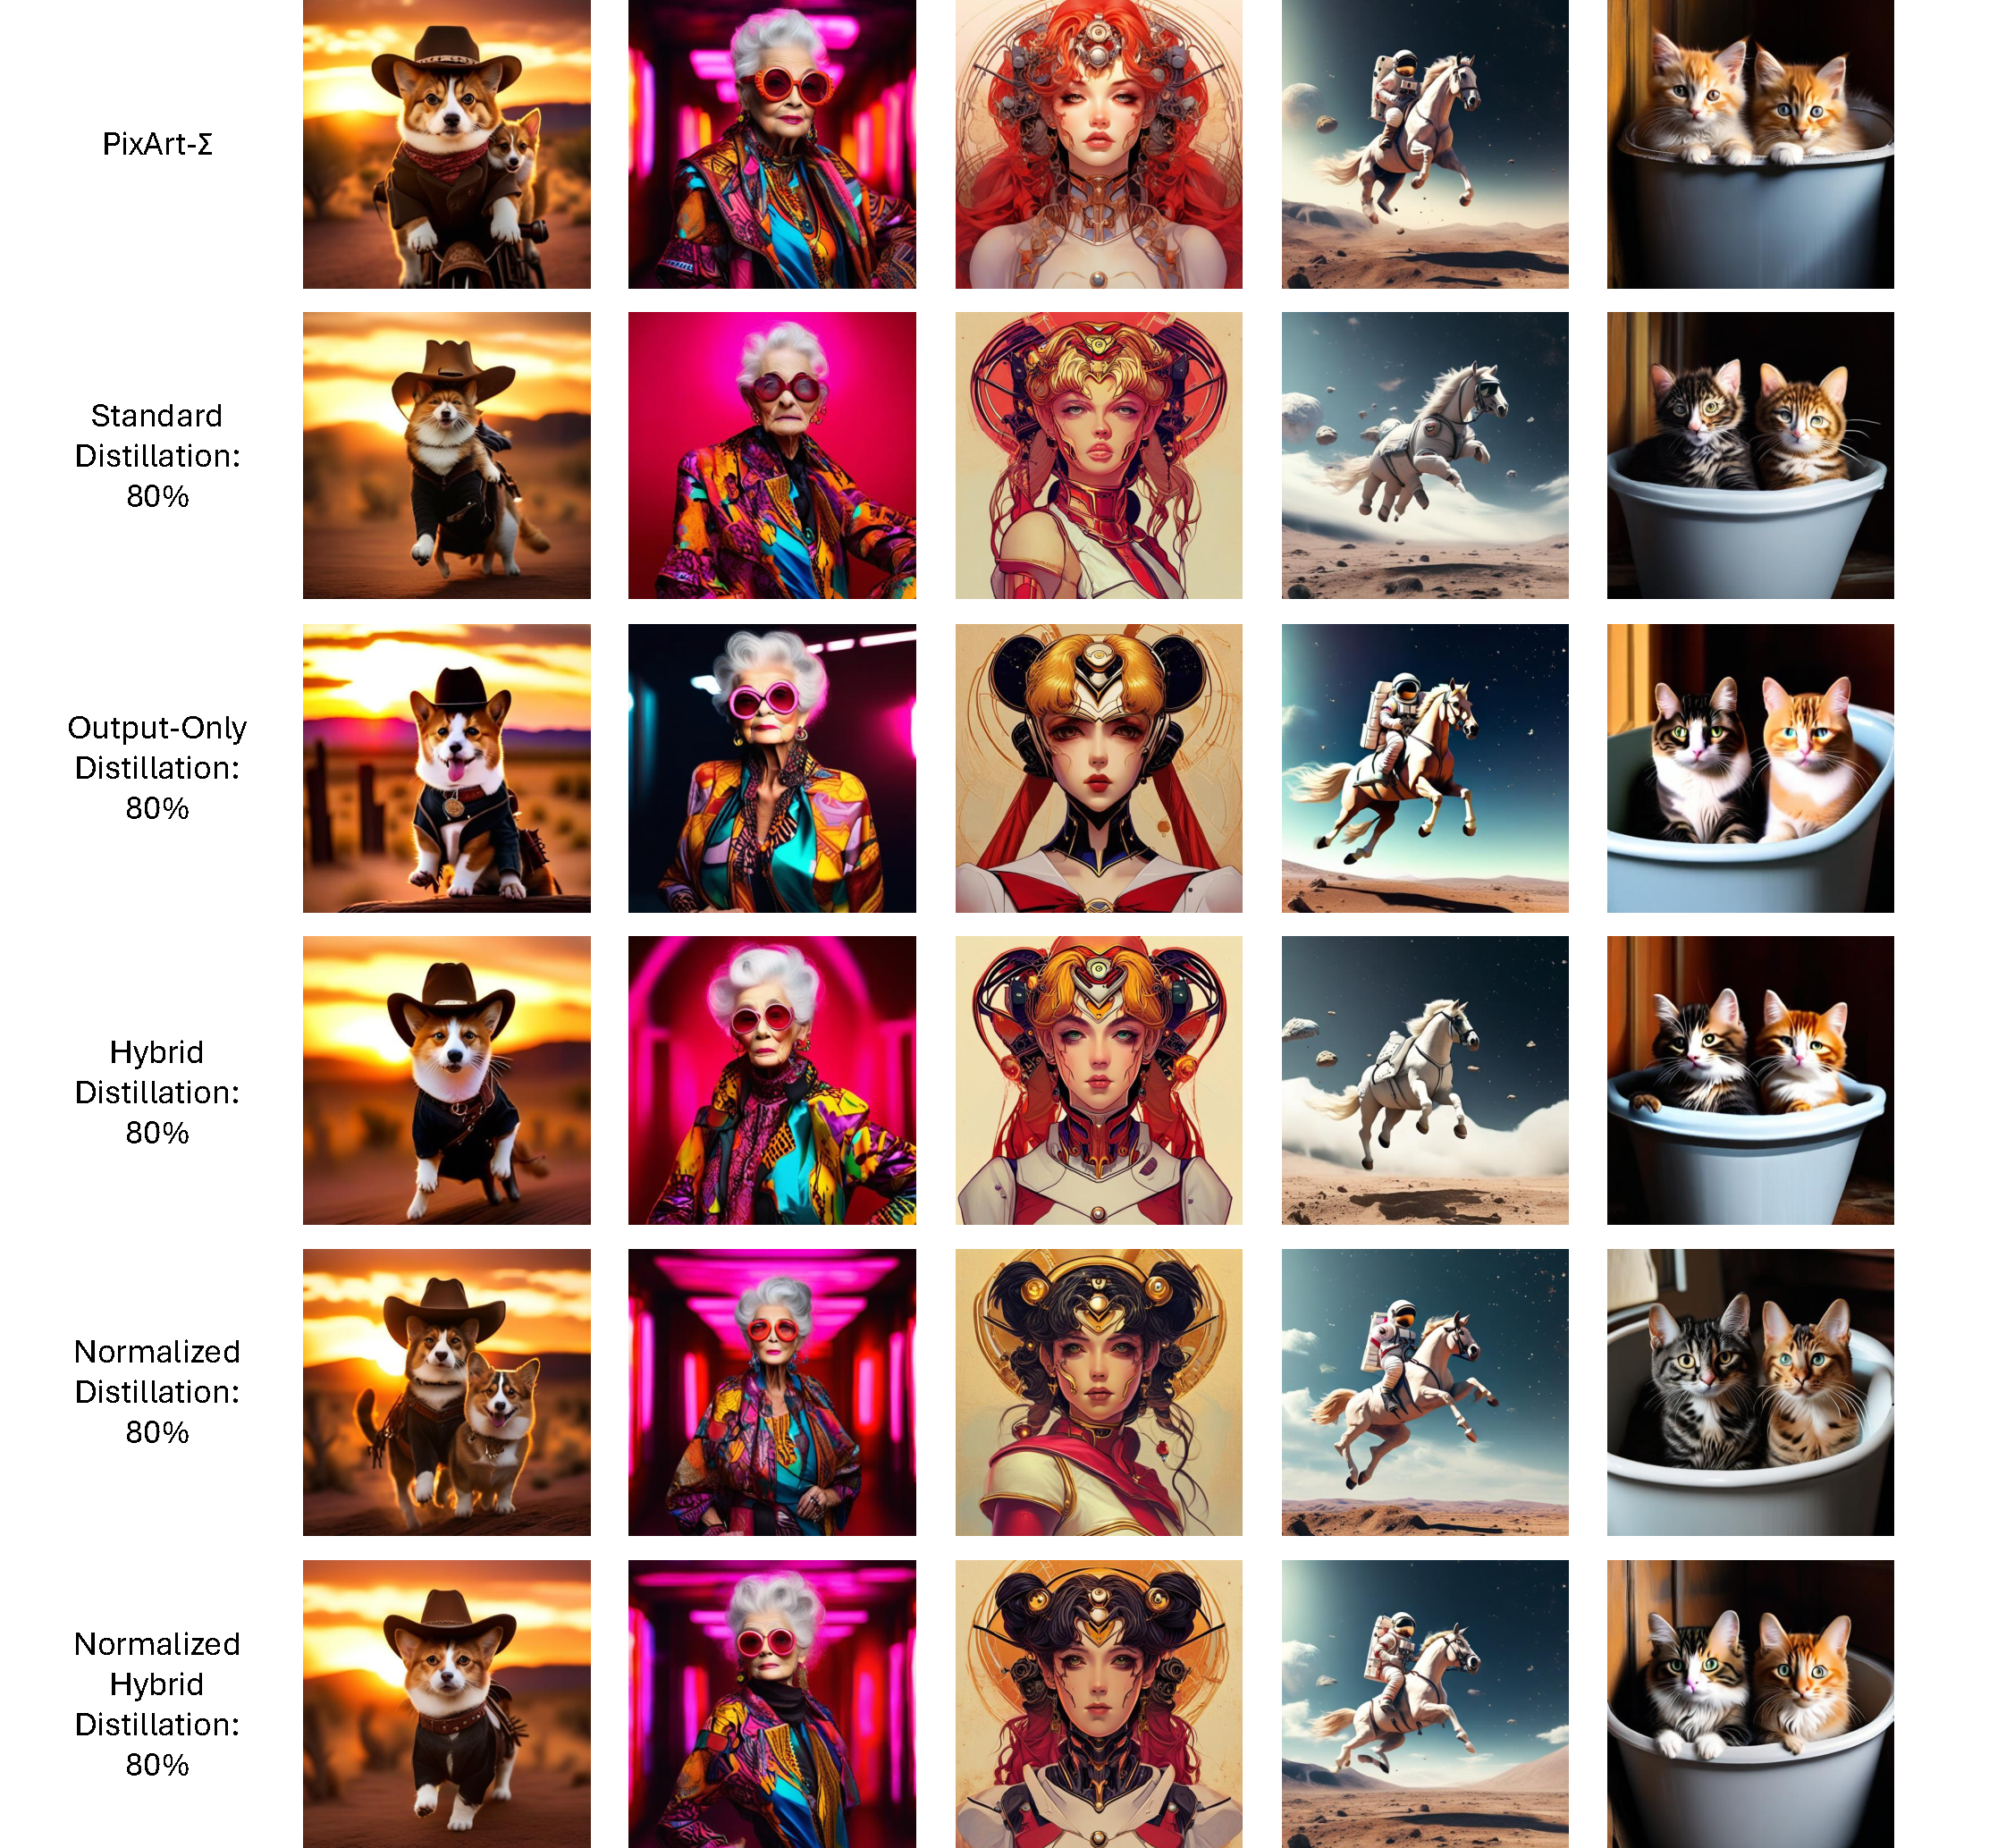
\includegraphics[width=0.65\textwidth]{images/Appendix/KnowledgeDistillation/model_80.pdf}
 	\caption[Qualitative Examples: Different Knowledge Distillation Loss Configurations (80\% Pruning)]{Qualitative comparison of example images generated by models pruned to 80\% using various knowledge distillation loss configurations}
	\label{fig:QualitativeLossInvestigation_80}
\end{figure}

\begin{figure}[H]
	\centering
	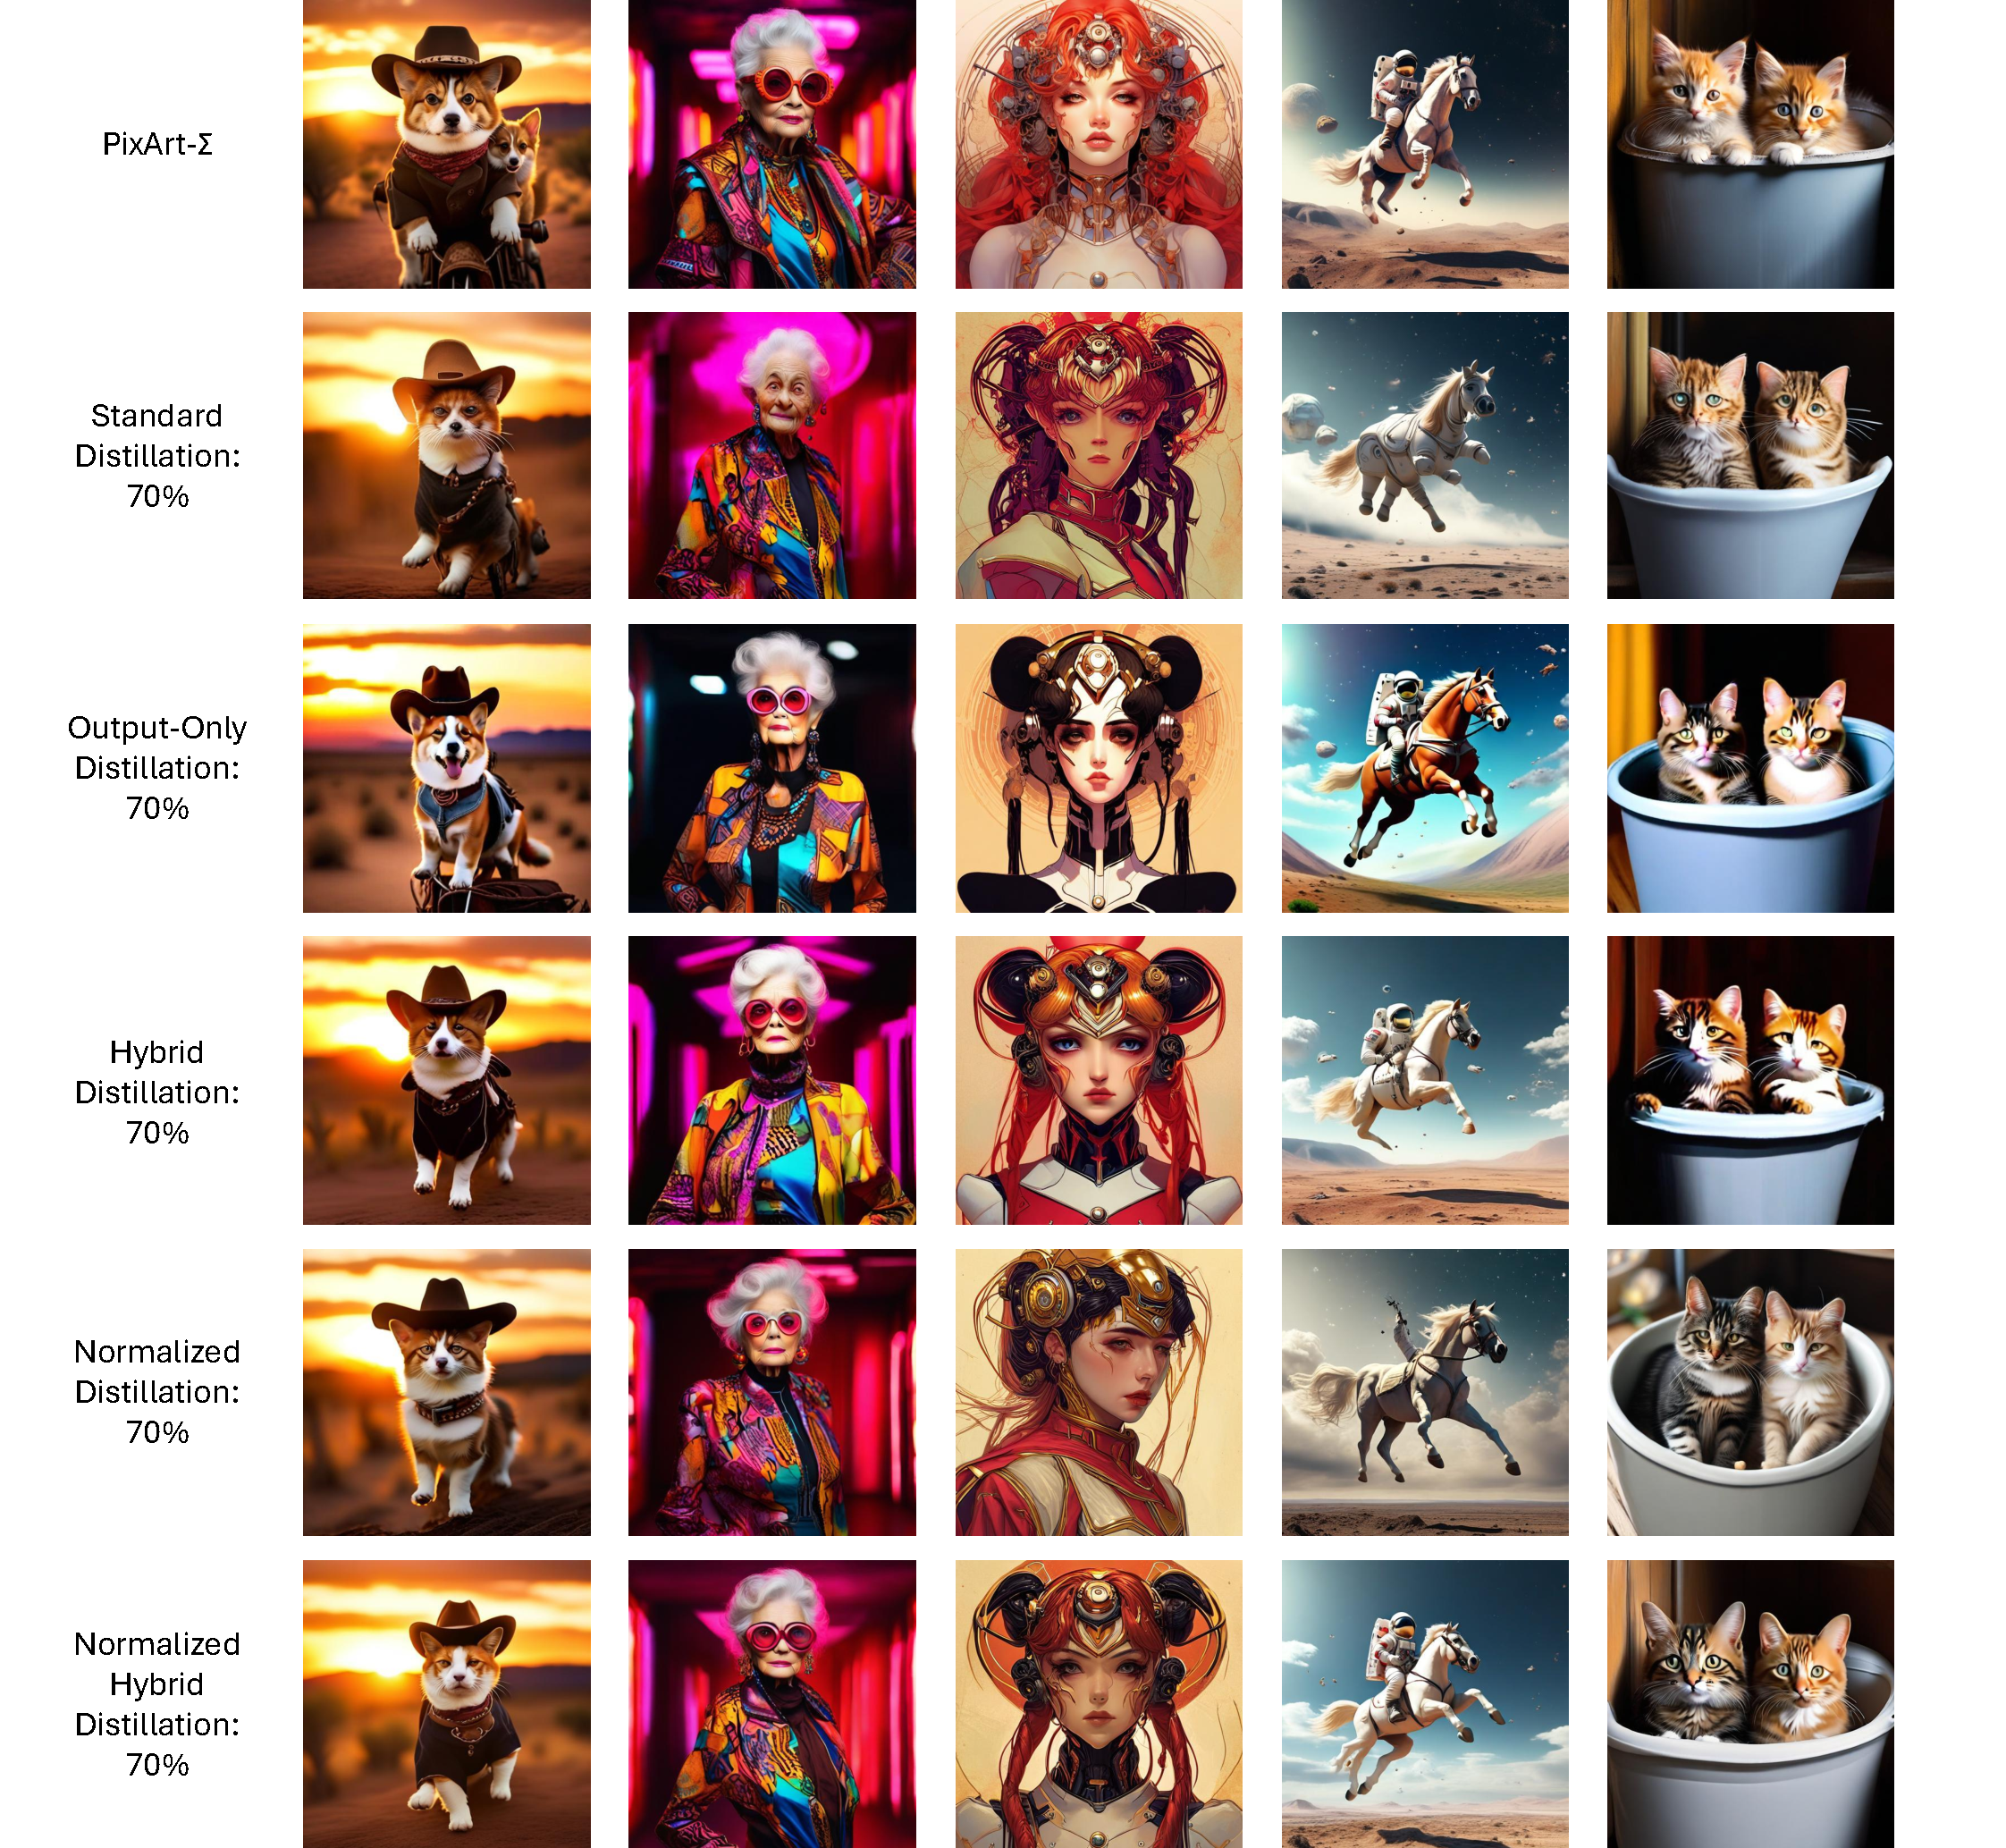
\includegraphics[width=0.65\textwidth]{images/Appendix/KnowledgeDistillation/model_70.pdf}
 	\caption[Qualitative Examples: Different Knowledge Distillation Loss Configurations (70\% Pruning)]{Qualitative comparison of example images generated by models pruned to 70\% using various knowledge distillation loss configurations}
	\label{fig:QualitativeLossInvestigation_70}
\end{figure}

\begin{figure}[H]
	\centering
	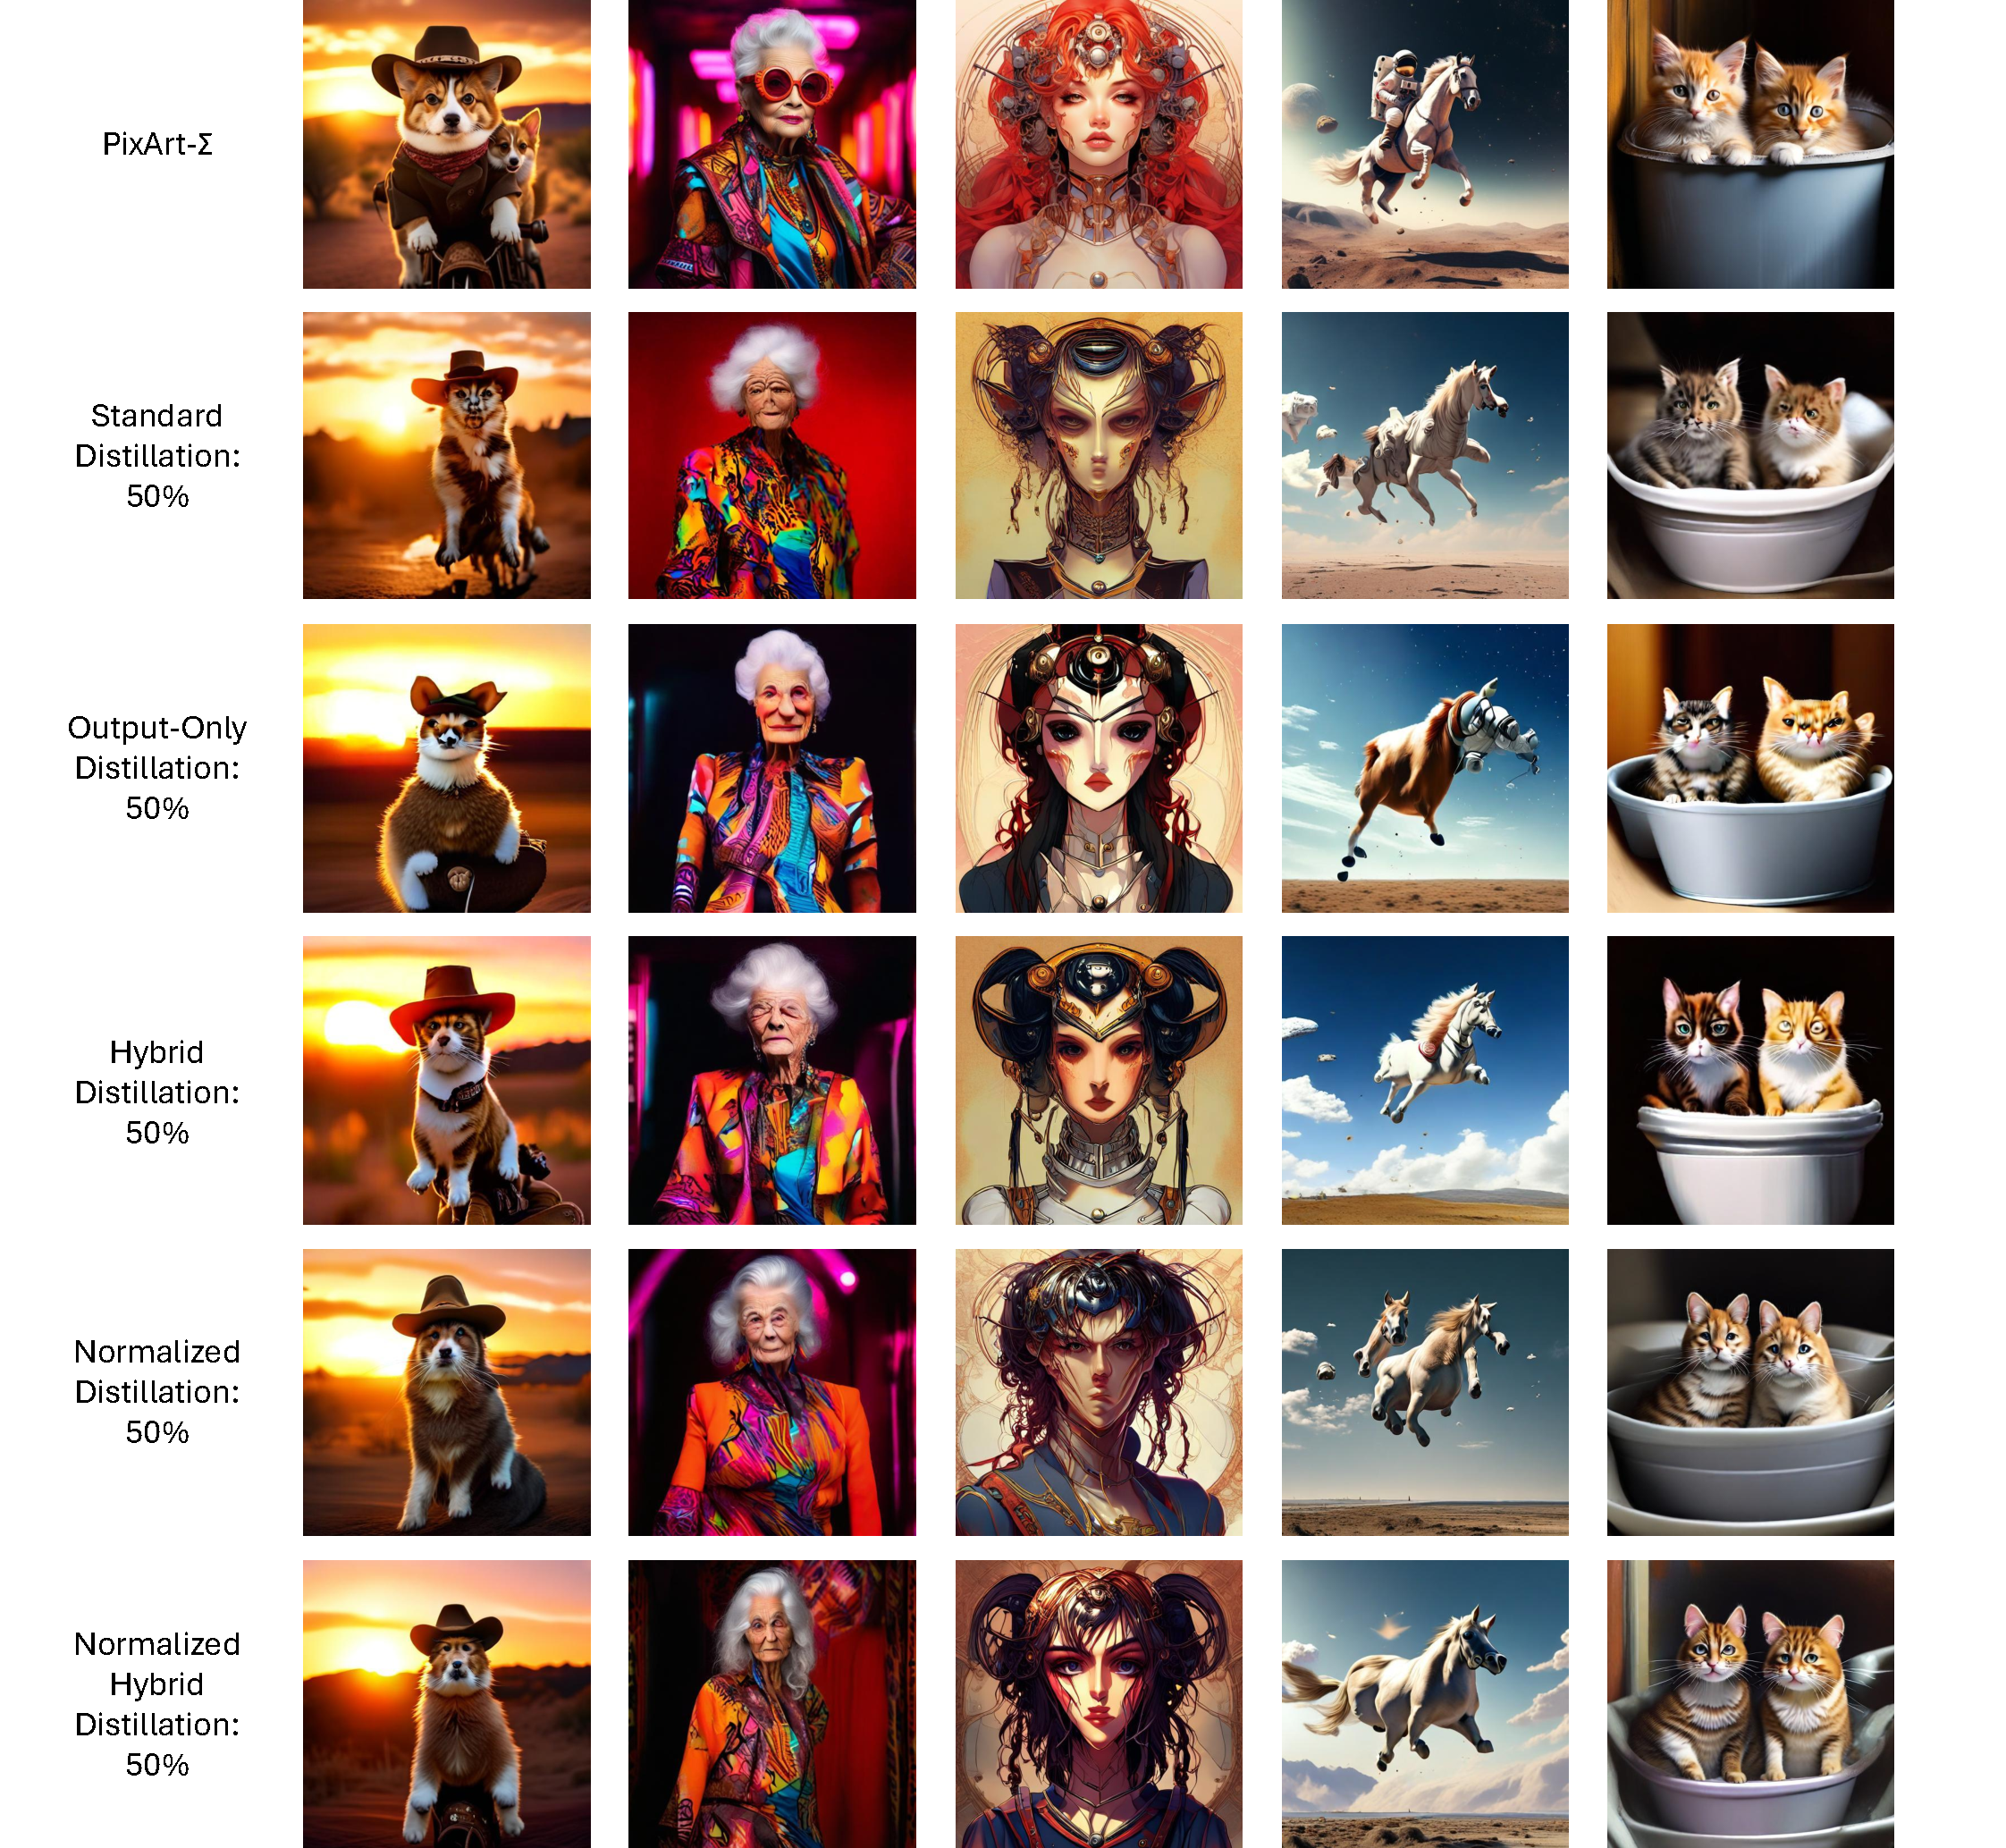
\includegraphics[width=0.65\textwidth]{images/Appendix/KnowledgeDistillation/model_50.pdf}
 	\caption[Qualitative Examples: Different Knowledge Distillation Loss Configurations (50\% Pruning)]{Qualitative comparison of example images generated by models pruned to 50\% using various knowledge distillation loss configurations}
	\label{fig:QualitativeLossInvestigation_50}
\end{figure}



\section{Fine-Tuning Protocol}
\label{sec:FinetuningProtocolAppendix}
In this section, qualitative examples are provided for the three fine-tuning protocols for PixArt-$\Sigma$ compressed to various sizes (Fig. \ref{fig:FinetuningProtocol_90} - \ref{fig:AppxFinetuningProtocol_50}).

\begin{figure}[H]
	\centering
	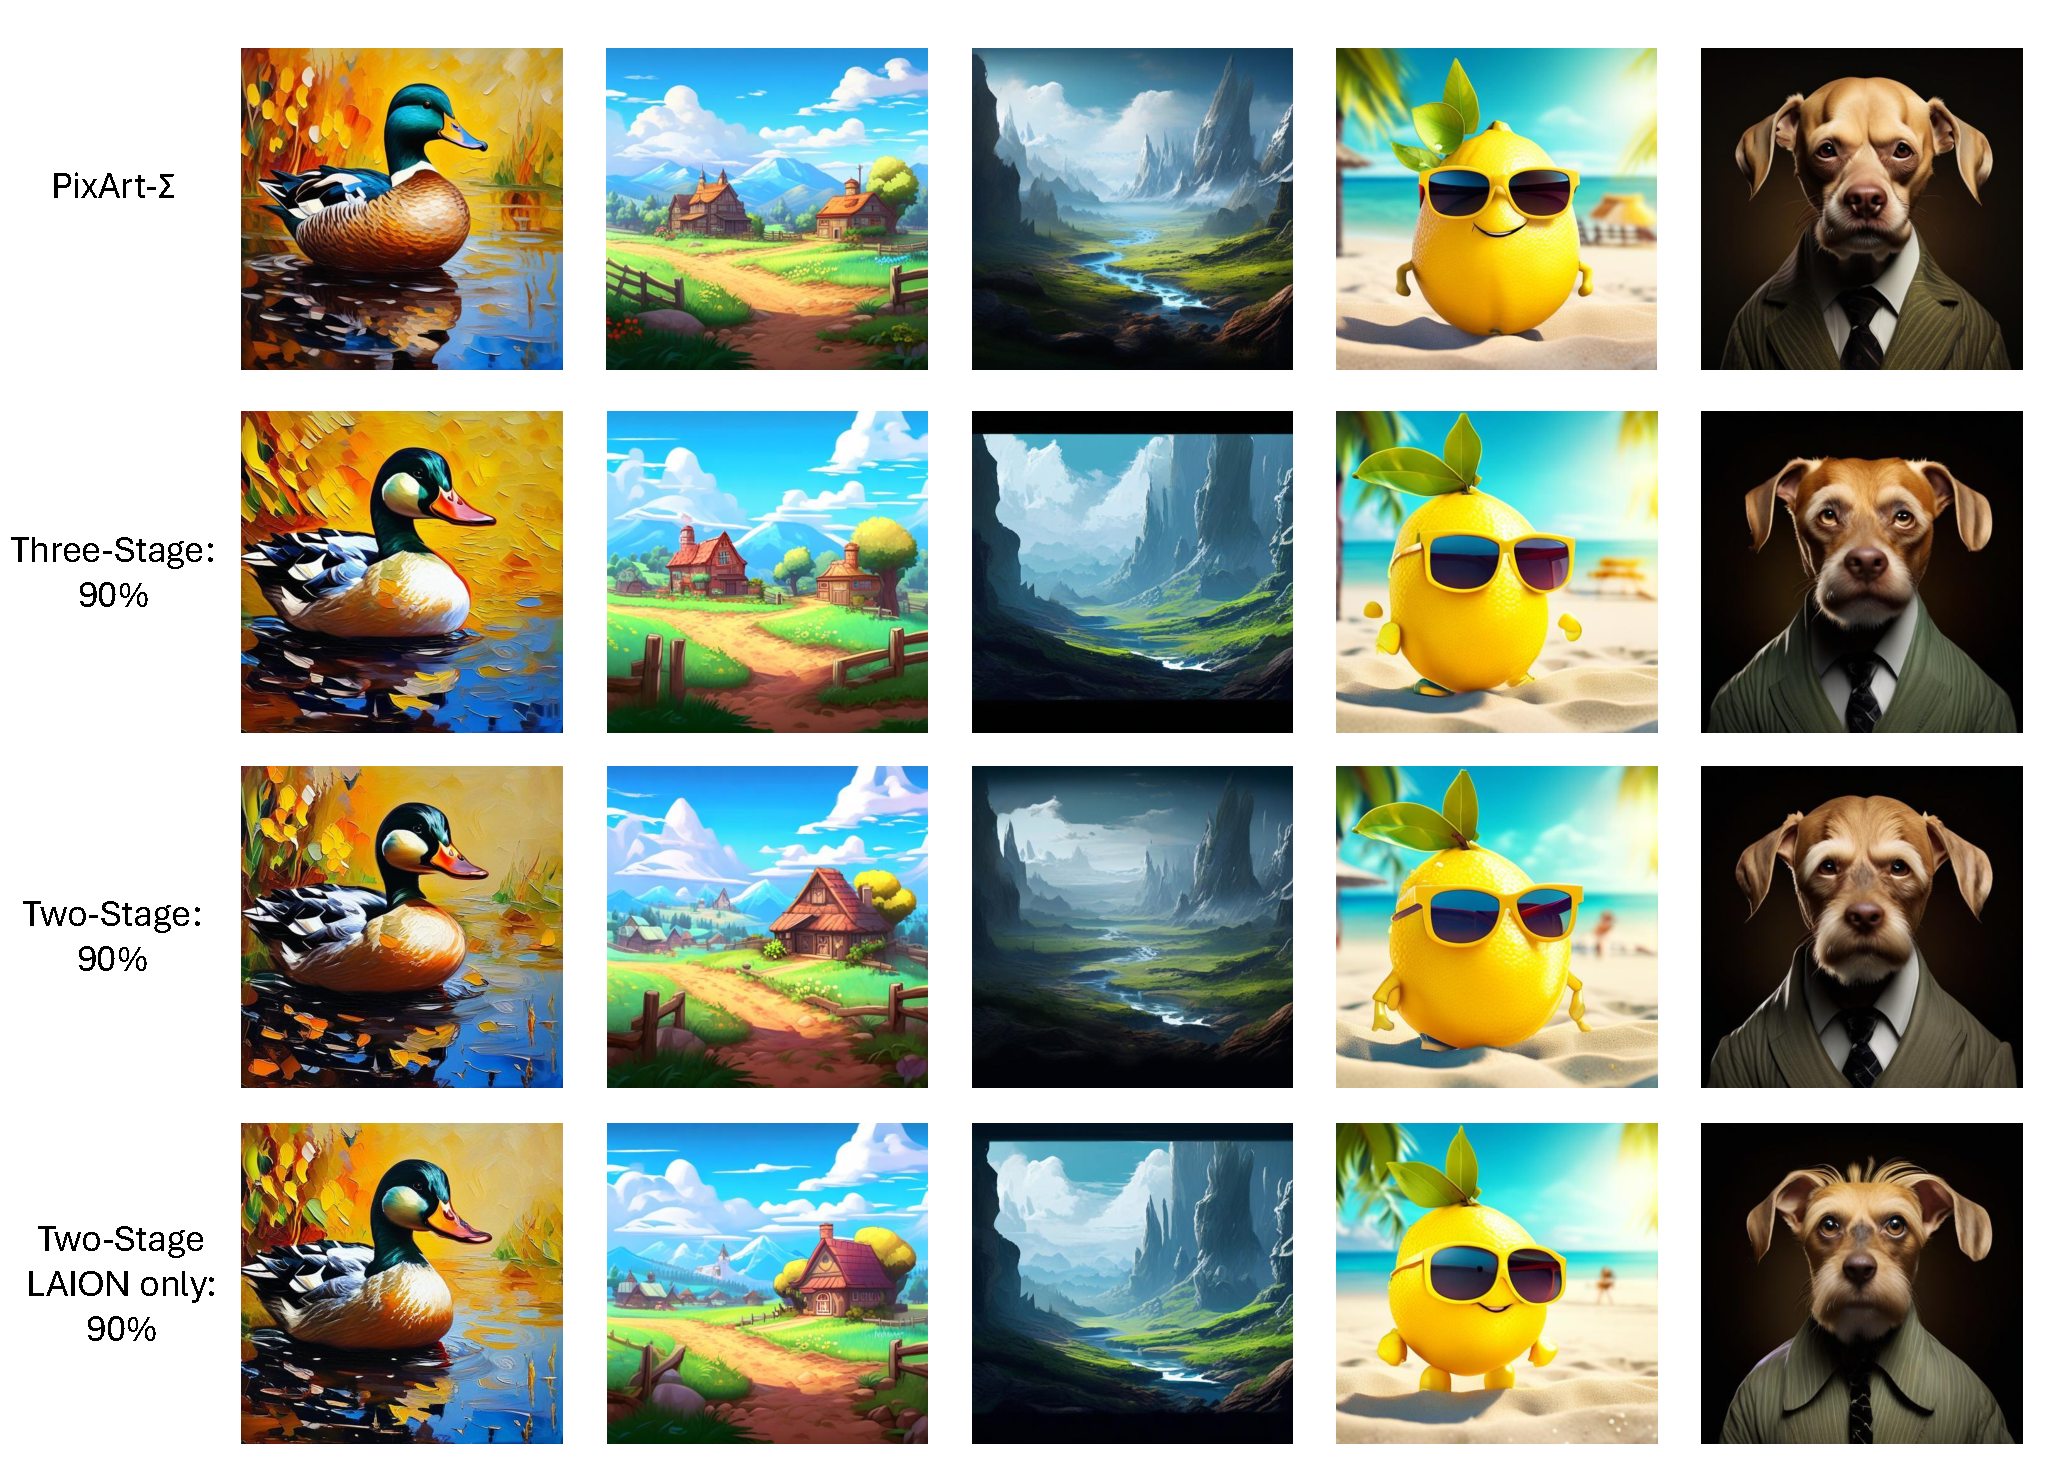
\includegraphics[width=0.7\textwidth]{images/Appendix/FinetuningProtocol/model_90.pdf}
 	\caption[Qualitative Examples: Fine-Tuning Protocols (90\% Pruning)]{Qualitative comparison of example images generated by models pruned to 90\% using various fine-tuning protocols.}
	\label{fig:FinetuningProtocol_90}
\end{figure}

\begin{figure}[H]
	\centering
	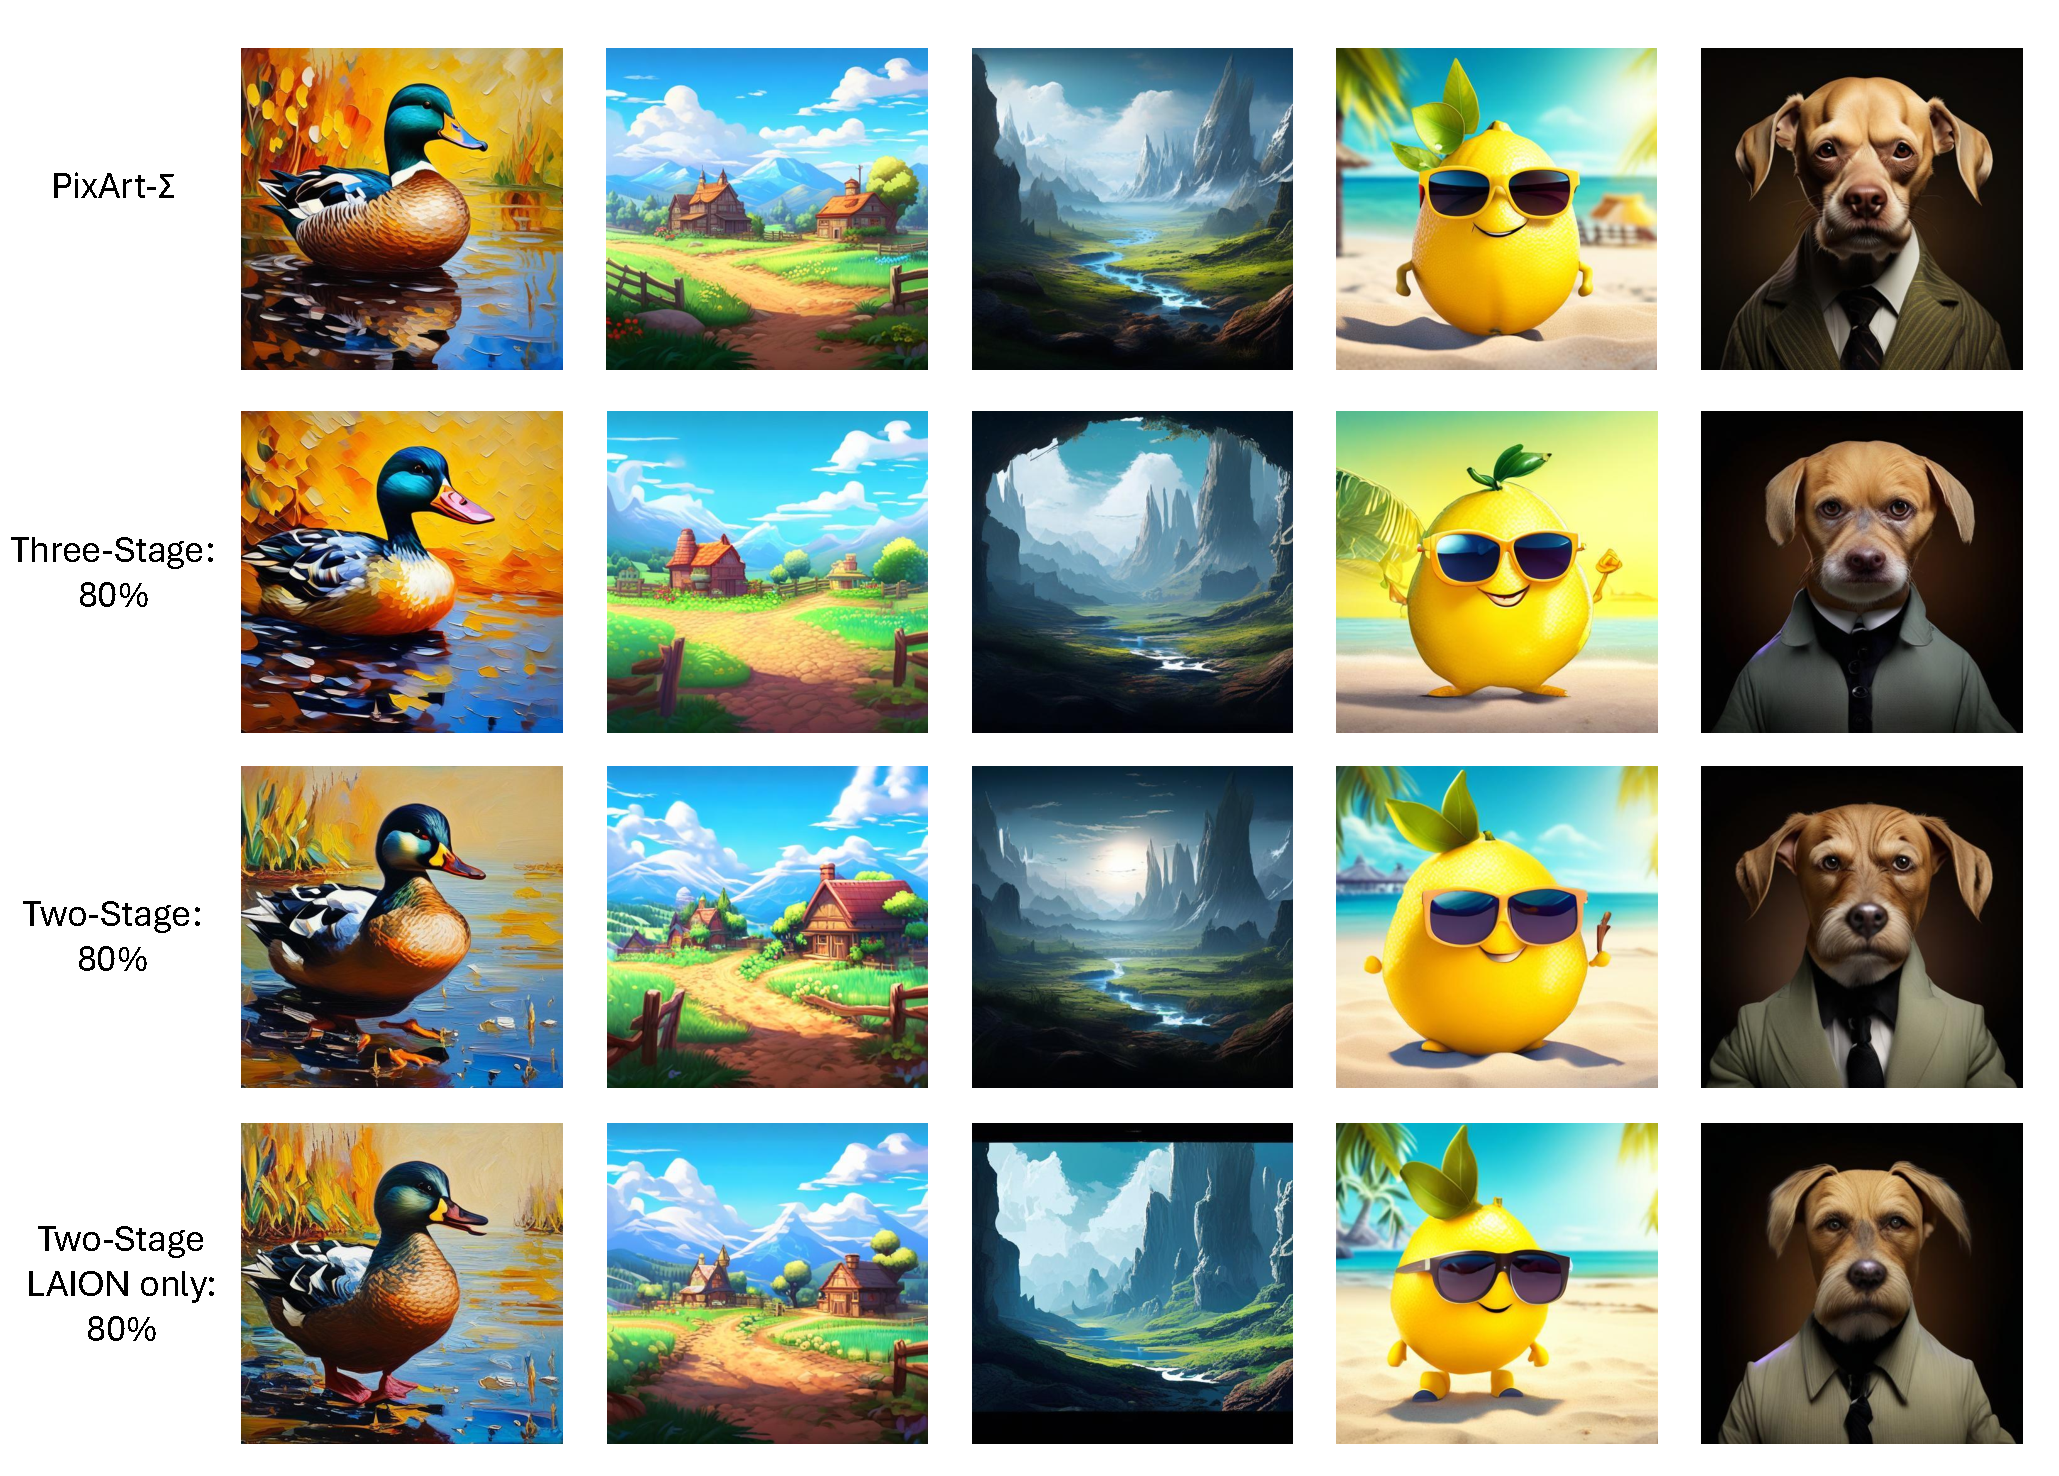
\includegraphics[width=0.7\textwidth]{images/Appendix/FinetuningProtocol/model_80.pdf}
 	\caption[Qualitative Examples: Fine-Tuning Protocols (80\% Pruning)]{Qualitative comparison of example images generated by models pruned to 80\% using various fine-tuning protocols.}
	\label{fig:AppxFinetuningProtocol_80}
\end{figure}

\begin{figure}[H]
	\centering
	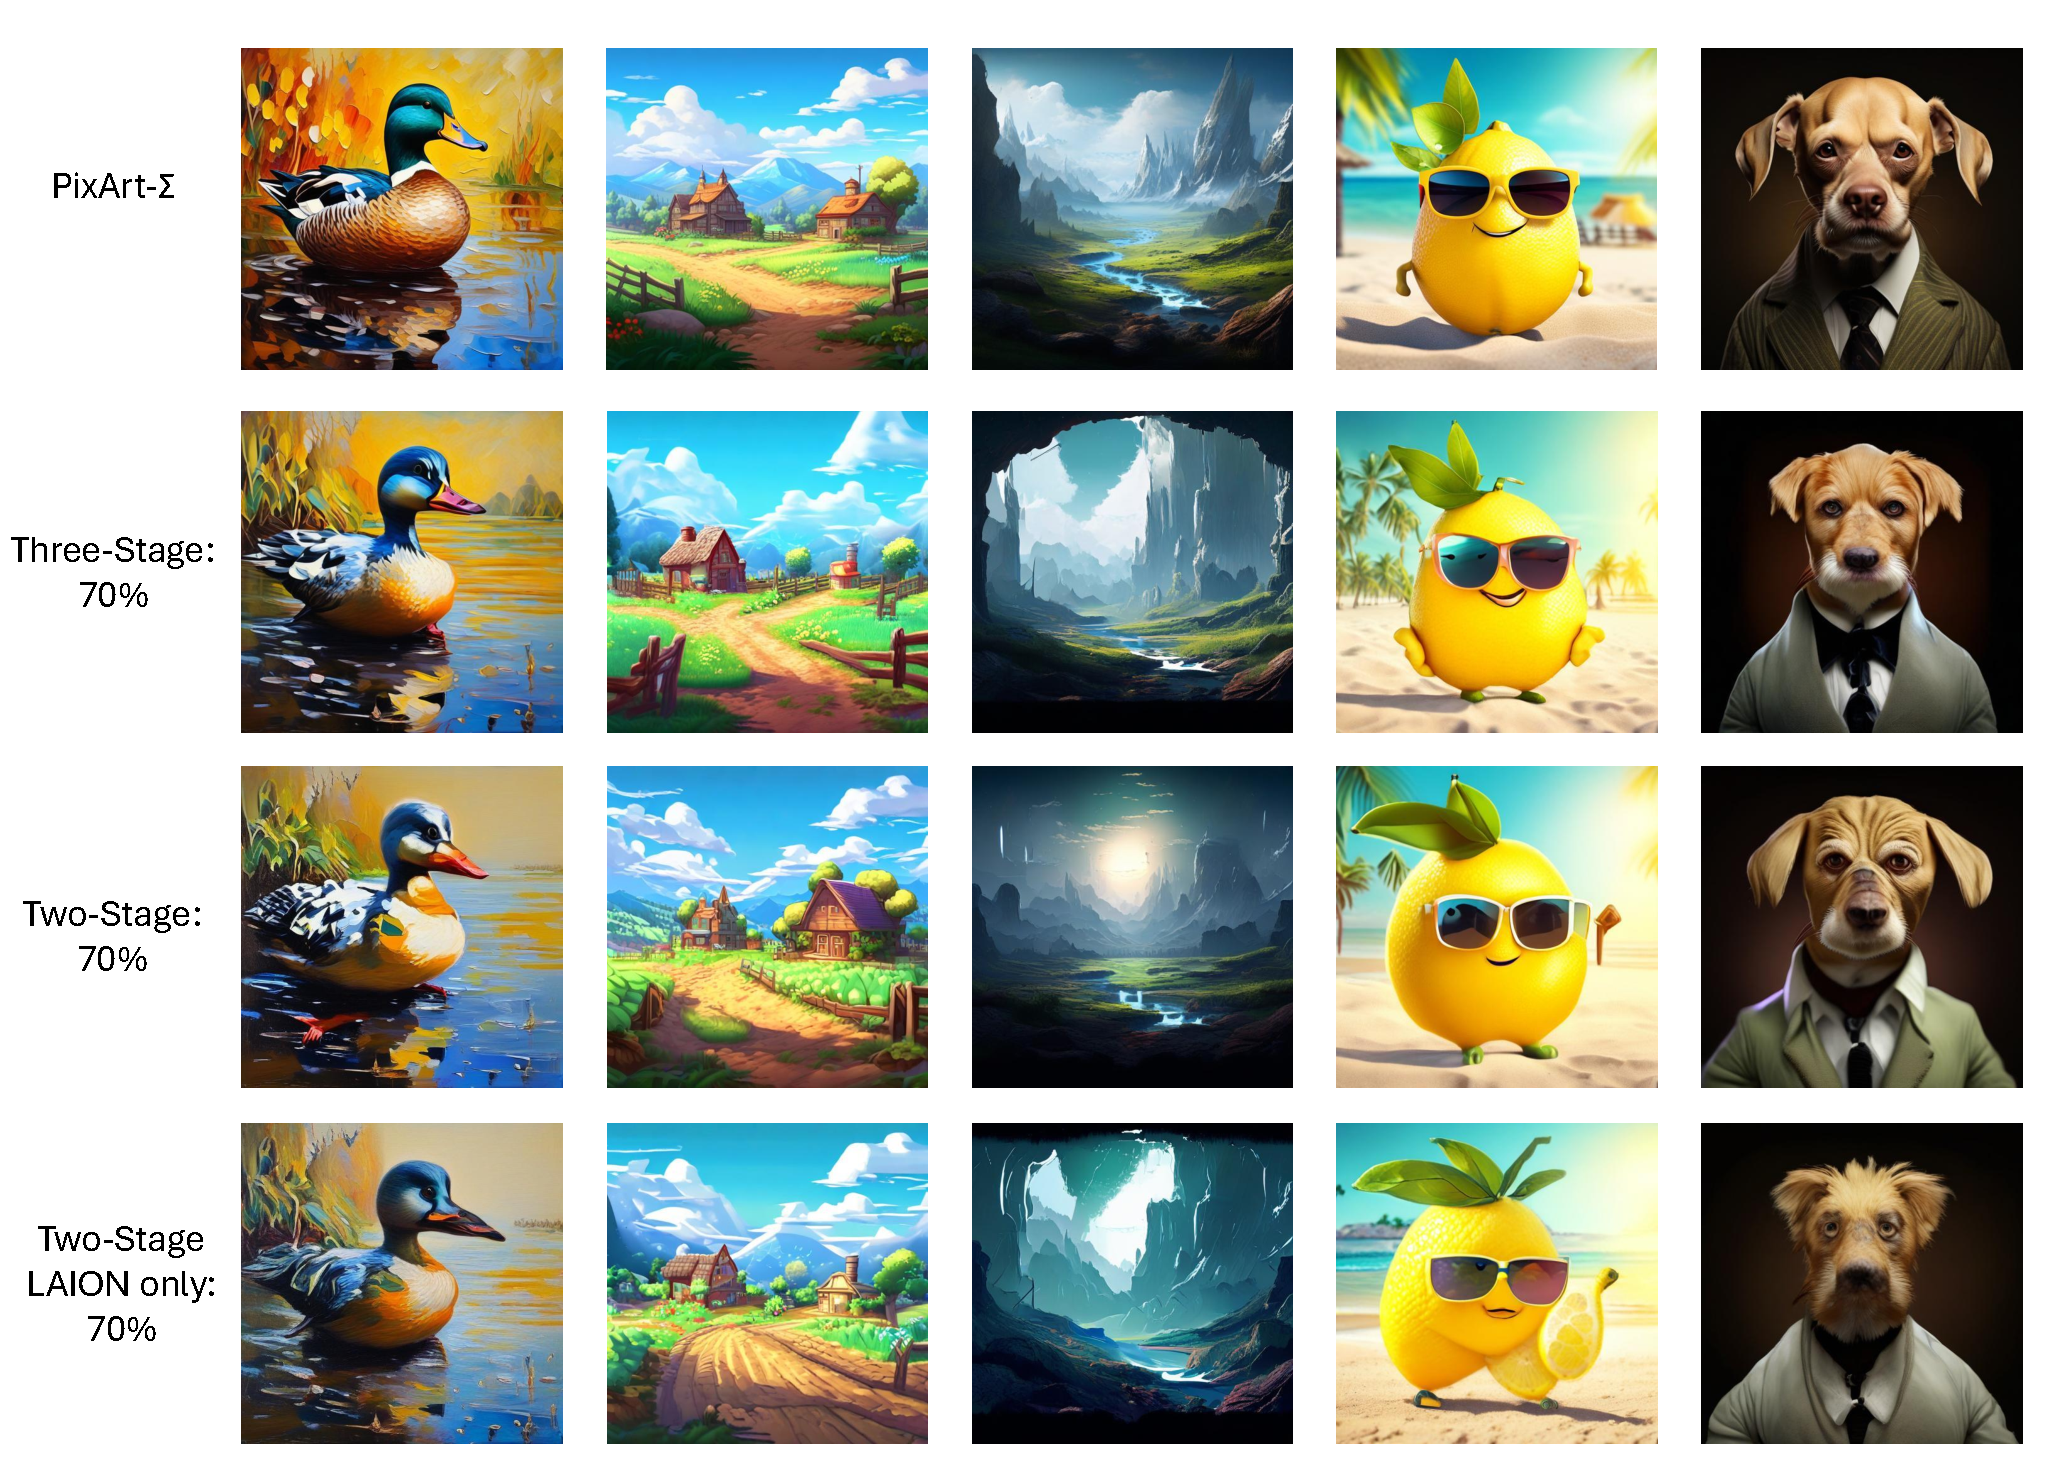
\includegraphics[width=0.7\textwidth]{images/Appendix/FinetuningProtocol/model_70.pdf}
 	\caption[Qualitative Examples: Fine-Tuning Protocols (70\% Pruning)]{Qualitative comparison of example images generated by models pruned to 70\% using various fine-tuning protocols.}
	\label{fig:AppxFinetuningProtocol_70}
\end{figure}

\begin{figure}[H]
	\centering
	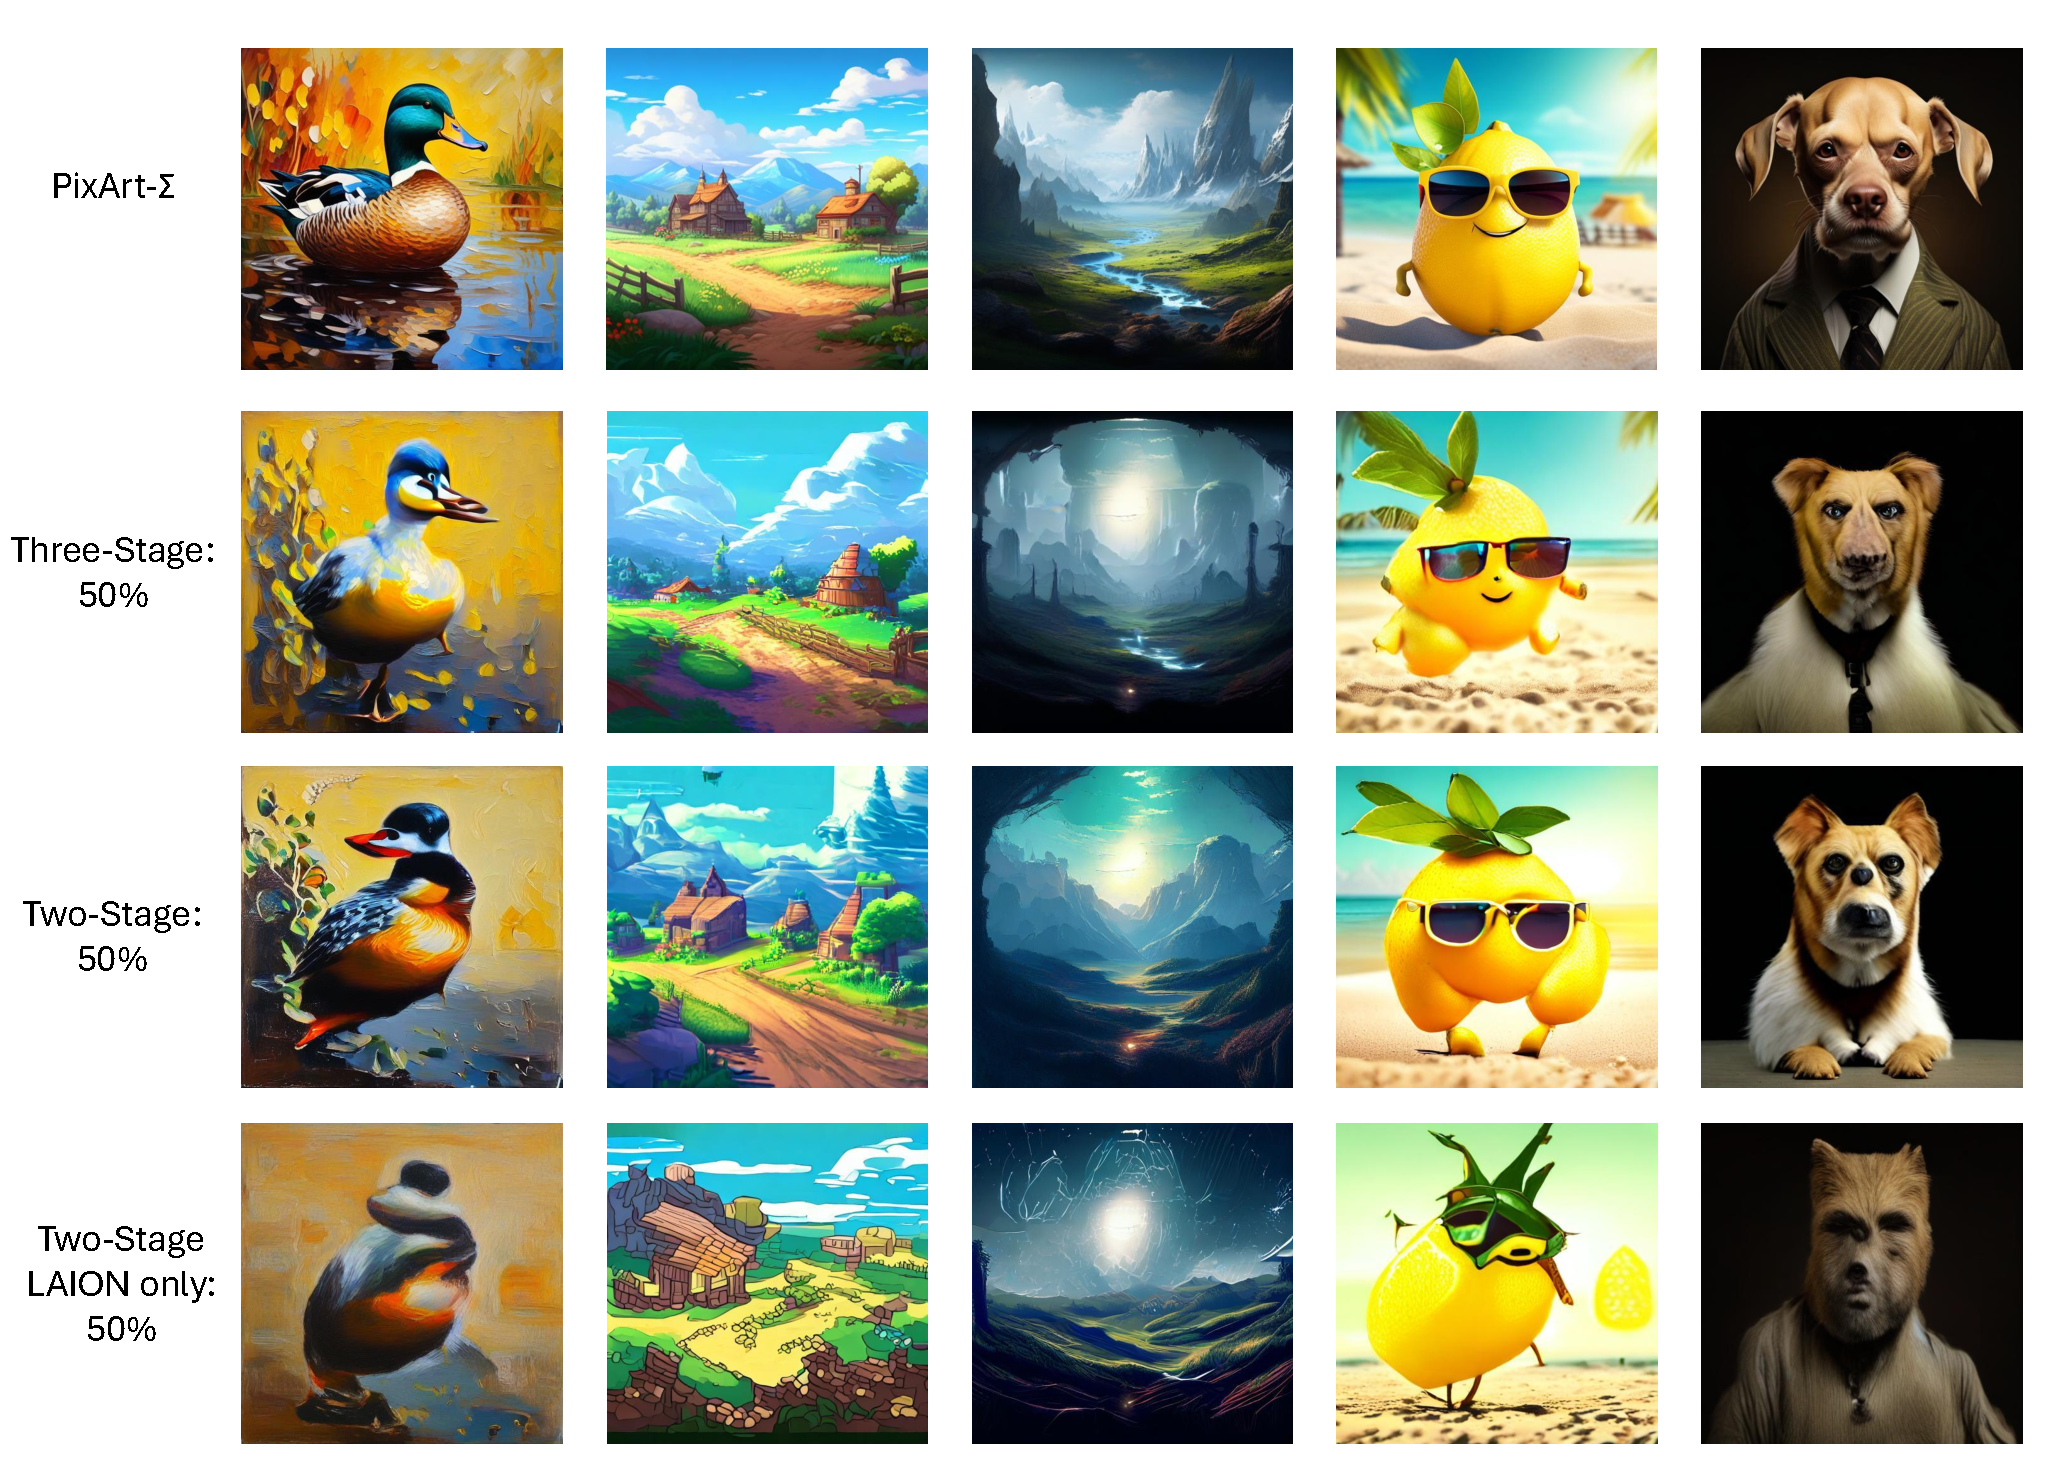
\includegraphics[width=0.7\textwidth]{images/Appendix/FinetuningProtocol/model_50.pdf}
 	\caption[Qualitative Examples: Fine-Tuning Protocols (50\% Pruning)]{Qualitative comparison of example images generated by models pruned to 50\% using various fine-tuning protocols.}
	\label{fig:AppxFinetuningProtocol_50}
\end{figure}


\section{Compression Strategy}
\label{appx:CompressionStrategy}
In this section, the PixArt-$\Sigma$ architecture with its compressed components is visualized (Fig. \ref{fig:PixArt_Sigma_Compresseed_Modules_Architecutre}). In addition, qualitative examples are provided comparing \gls{SVD}-based compression with complete block removal (Fig. \ref{fig:Example_Images_SVD_vs_Removal_90_Appx} - \ref{fig:Example_Images_SVD_vs_Removal_60_Appx}).

   	\begin{figure}[H]
	\centering
	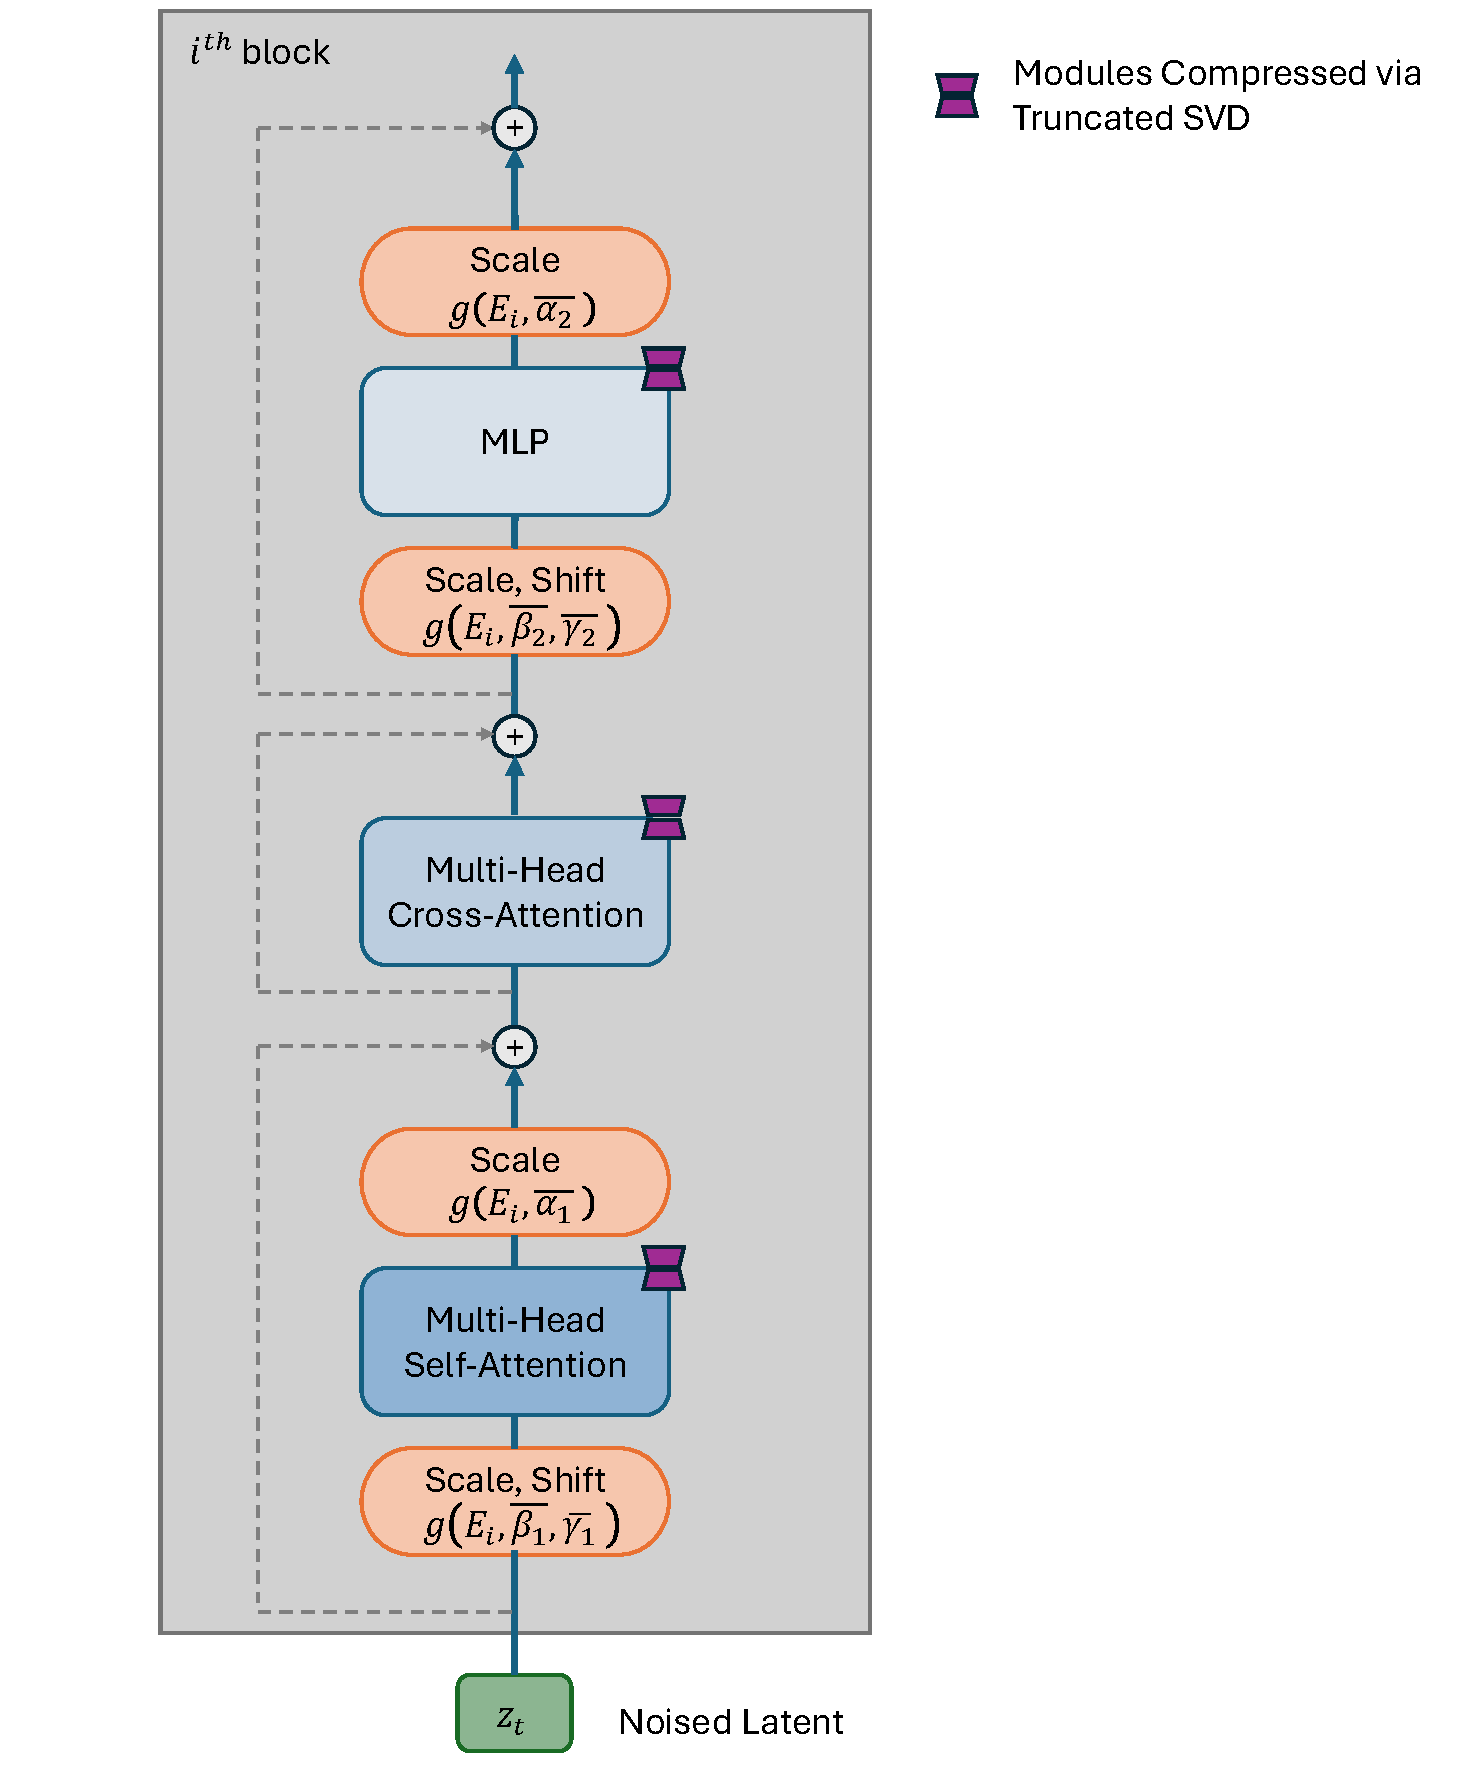
\includegraphics[width=0.5\textwidth]{images/Experimente/SVD_VS_Removal/PixartArchitectureCompressedModules.pdf}
	\caption[PixArt-$\Sigma$ compressed modules.]{PixArt-$\Sigma$ compressed modules.}
	\label{fig:PixArt_Sigma_Compresseed_Modules_Architecutre}
\end{figure}

   	\begin{figure}[H]
	\centering
	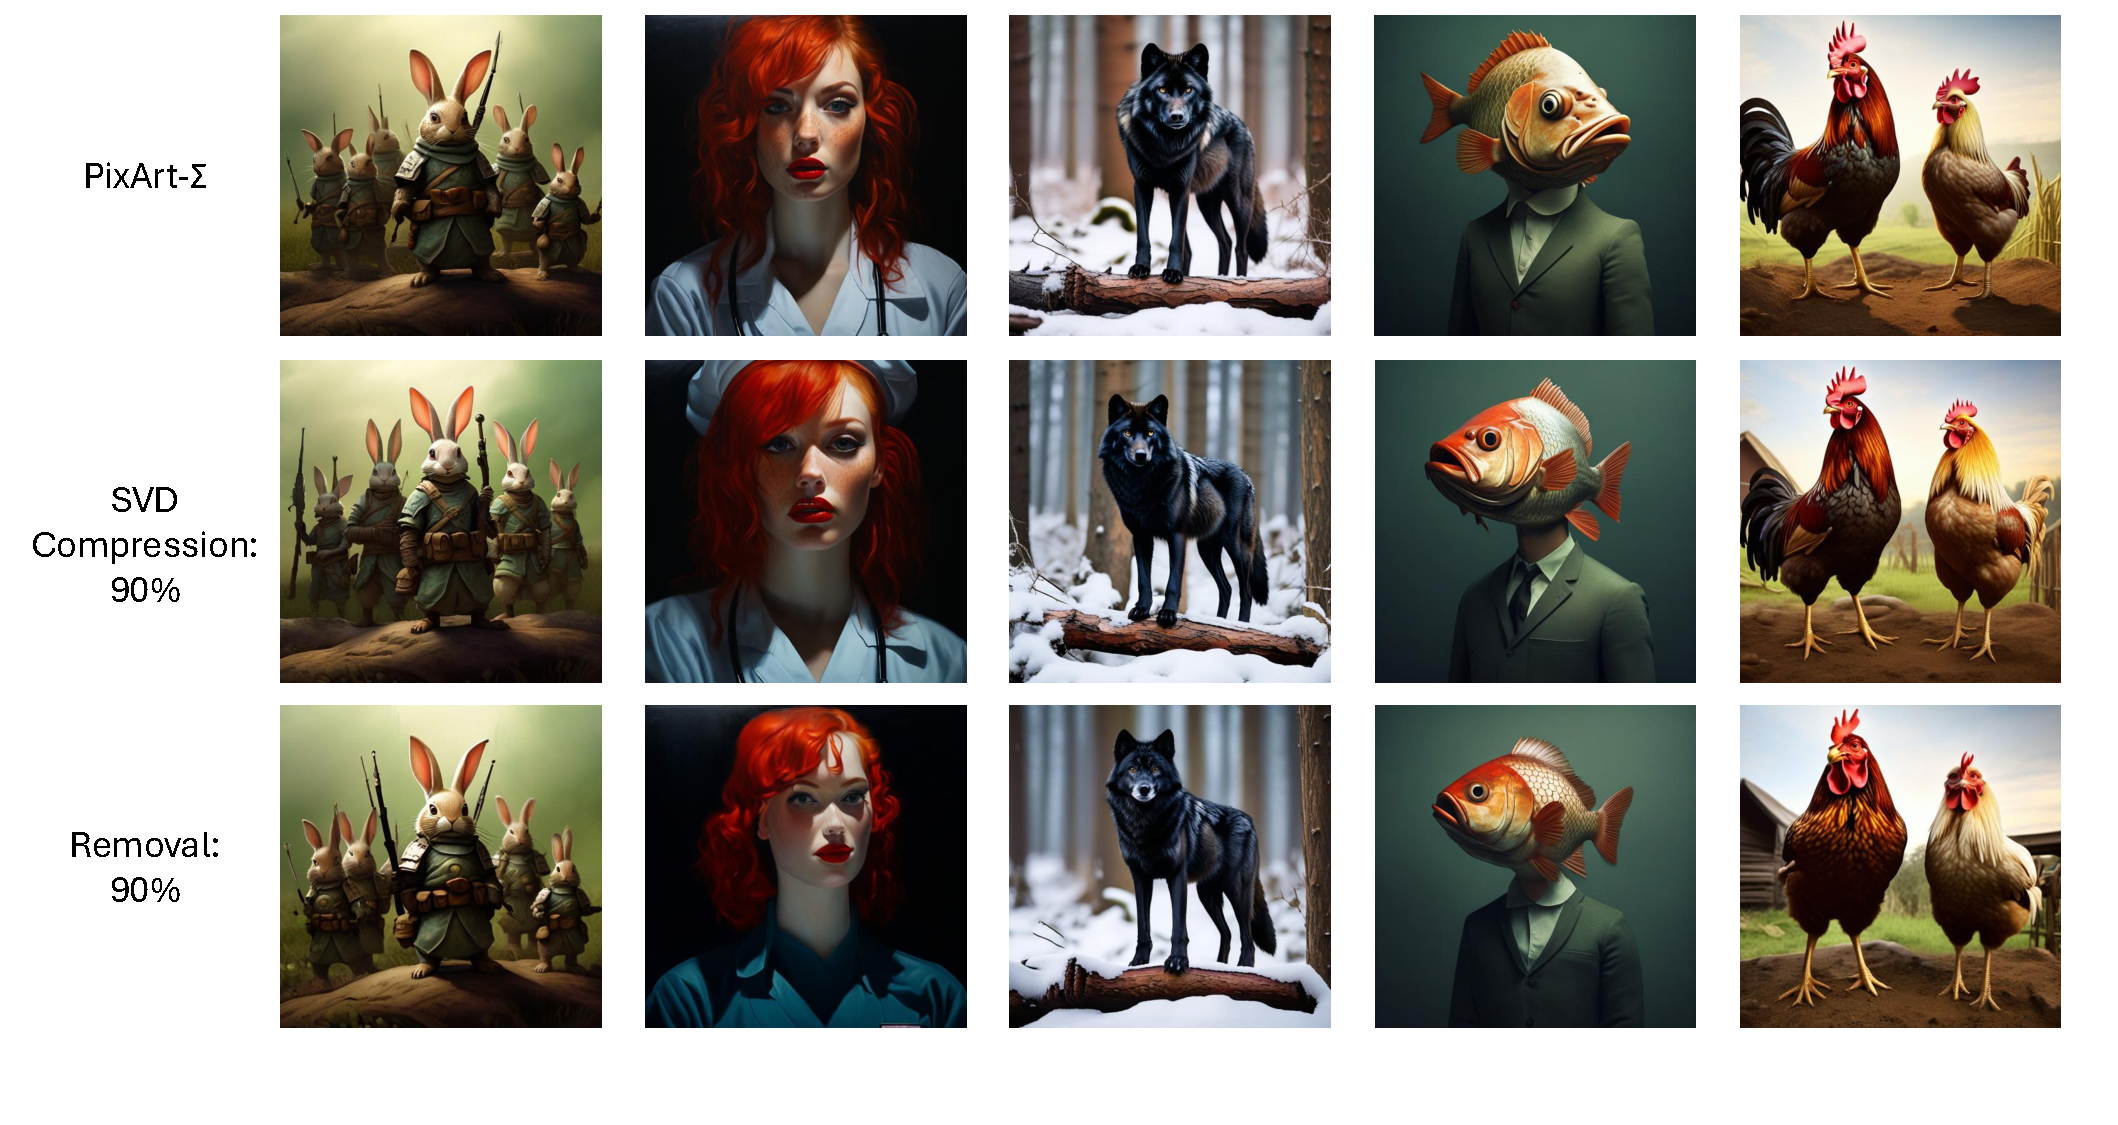
\includegraphics[width=0.9\textwidth]{images/Experimente/SVD_VS_Removal/ImageExamples_model90.pdf}
 	\caption[Qualitative Examples: Compression Strategies (90\% Pruning)]{Qualitative comparison of example images generated by models pruned to 90\% using complete block removal versus \gls{SVD}-based block compression.}
	\label{fig:Example_Images_SVD_vs_Removal_90_Appx}
\end{figure}

   	\begin{figure}[H]
	\centering
	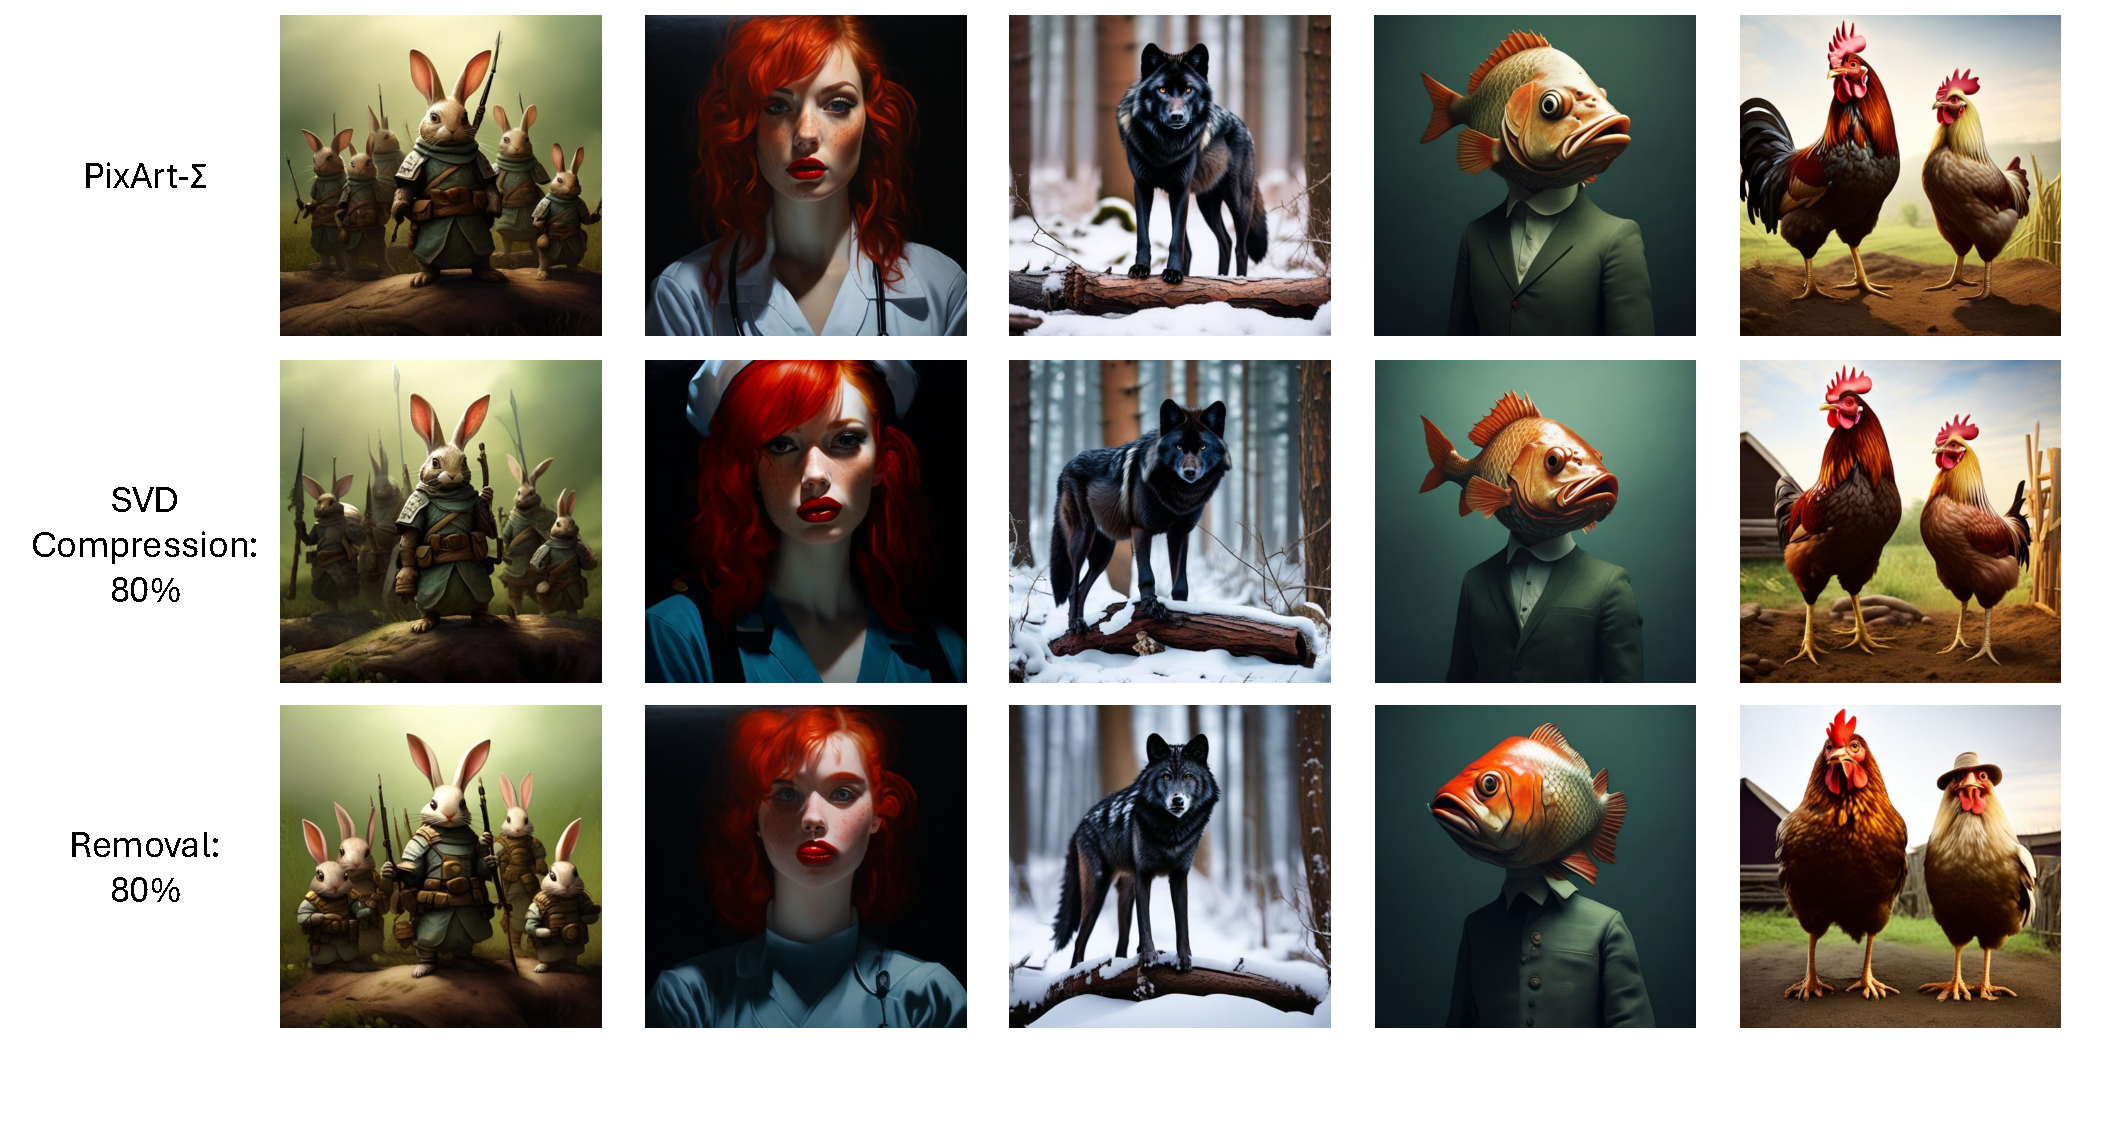
\includegraphics[width=0.9\textwidth]{images/Experimente/SVD_VS_Removal/ImageExamples_model80.pdf}
 	\caption[Qualitative Examples: Compression Strategies (80\% Pruning)]{Qualitative comparison of example images generated by models pruned to 80\% using complete block removal versus \gls{SVD}-based block compression.}
	\label{fig:Example_Images_SVD_vs_Removal_80_Appx}
\end{figure}

   	\begin{figure}[H]
	\centering
	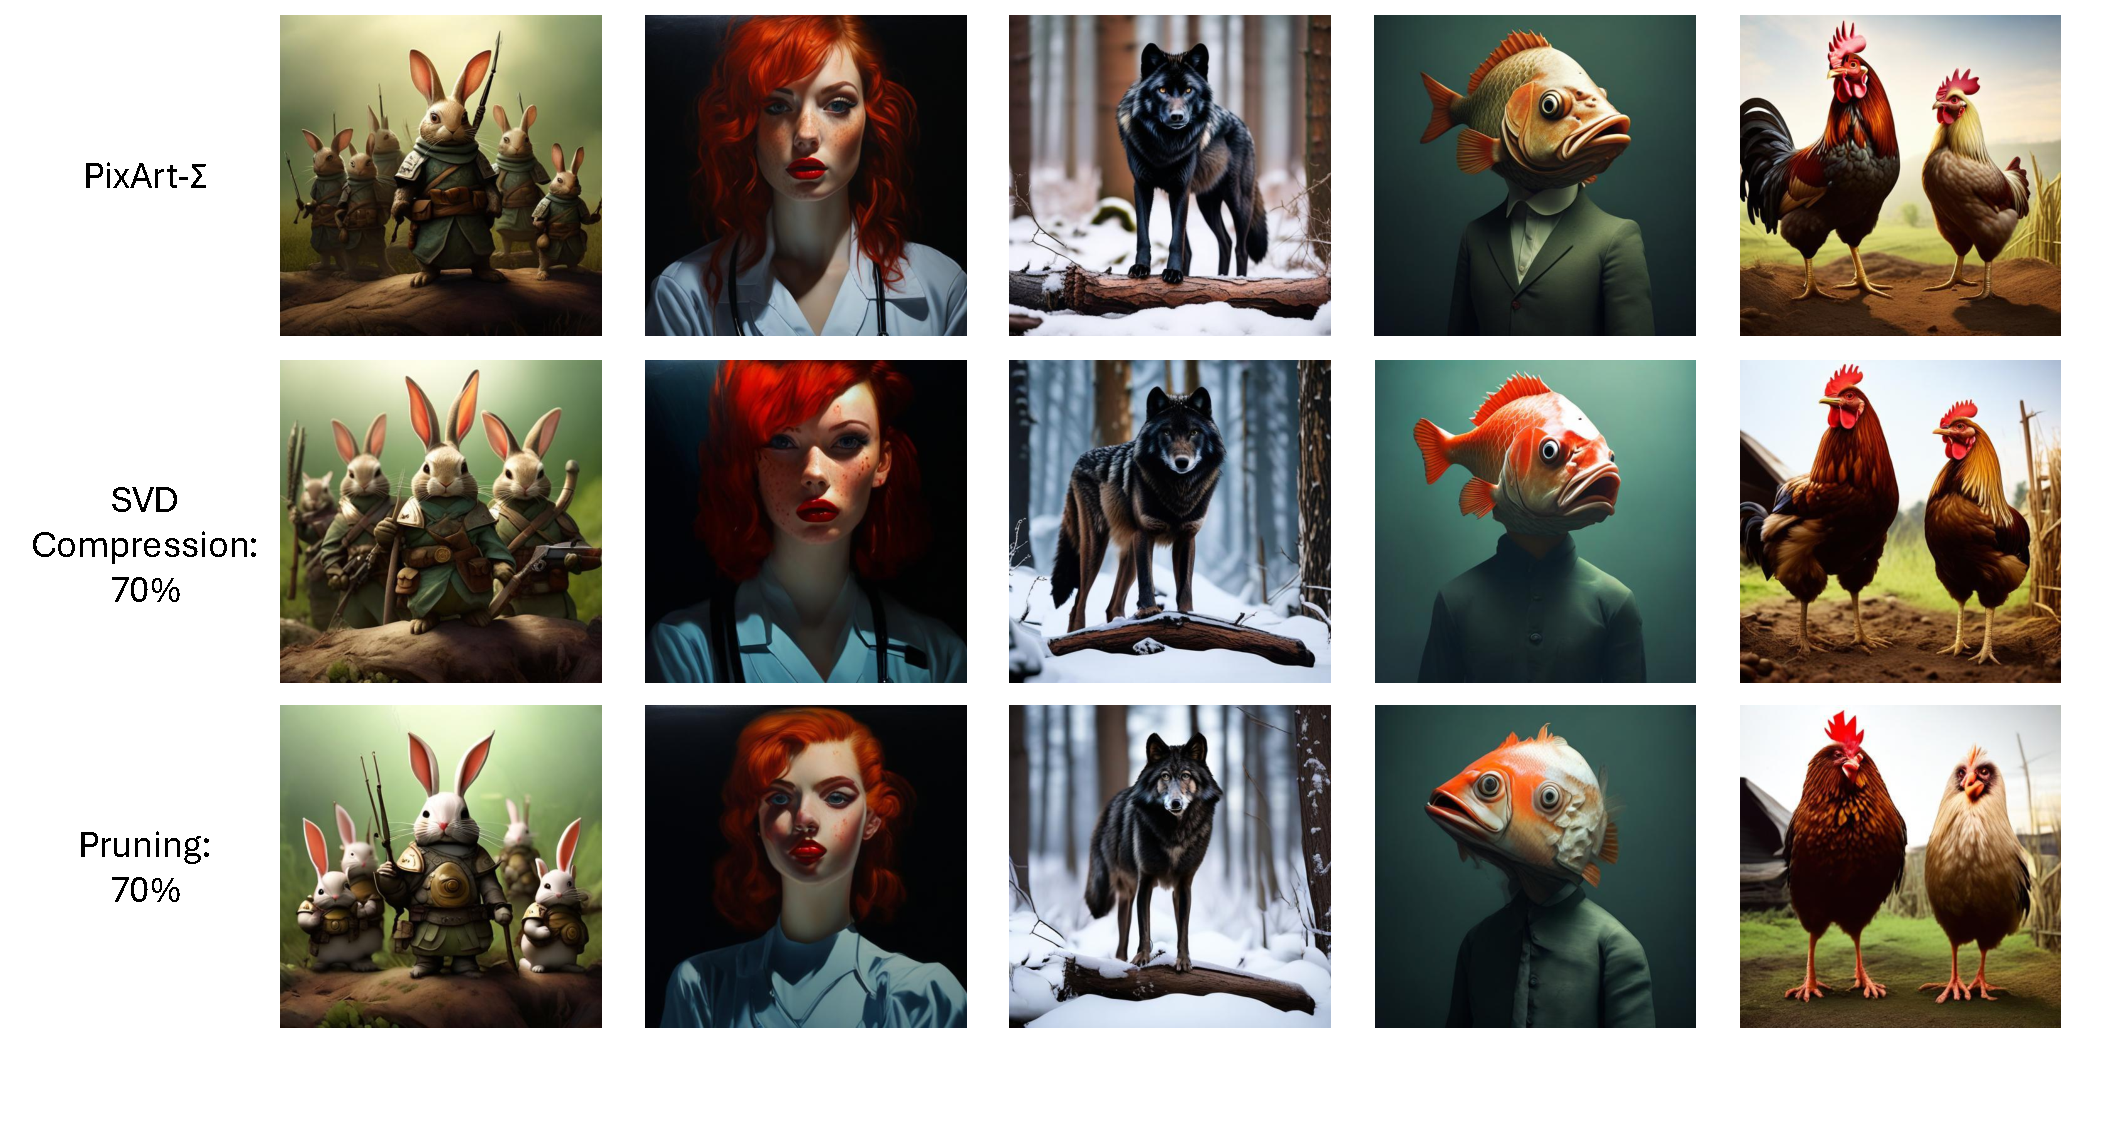
\includegraphics[width=0.9\textwidth]{images/Experimente/SVD_VS_Removal/ImageExamples_model70.pdf}
 	\caption[Qualitative Examples: Compression Strategies (70\% Pruning)]{Qualitative comparison of example images generated by models pruned to 70\% using complete block removal versus \gls{SVD}-based block compression.}
	\label{fig:Example_Images_SVD_vs_Removal_70_Appx}
\end{figure}

   	\begin{figure}[H]
	\centering
	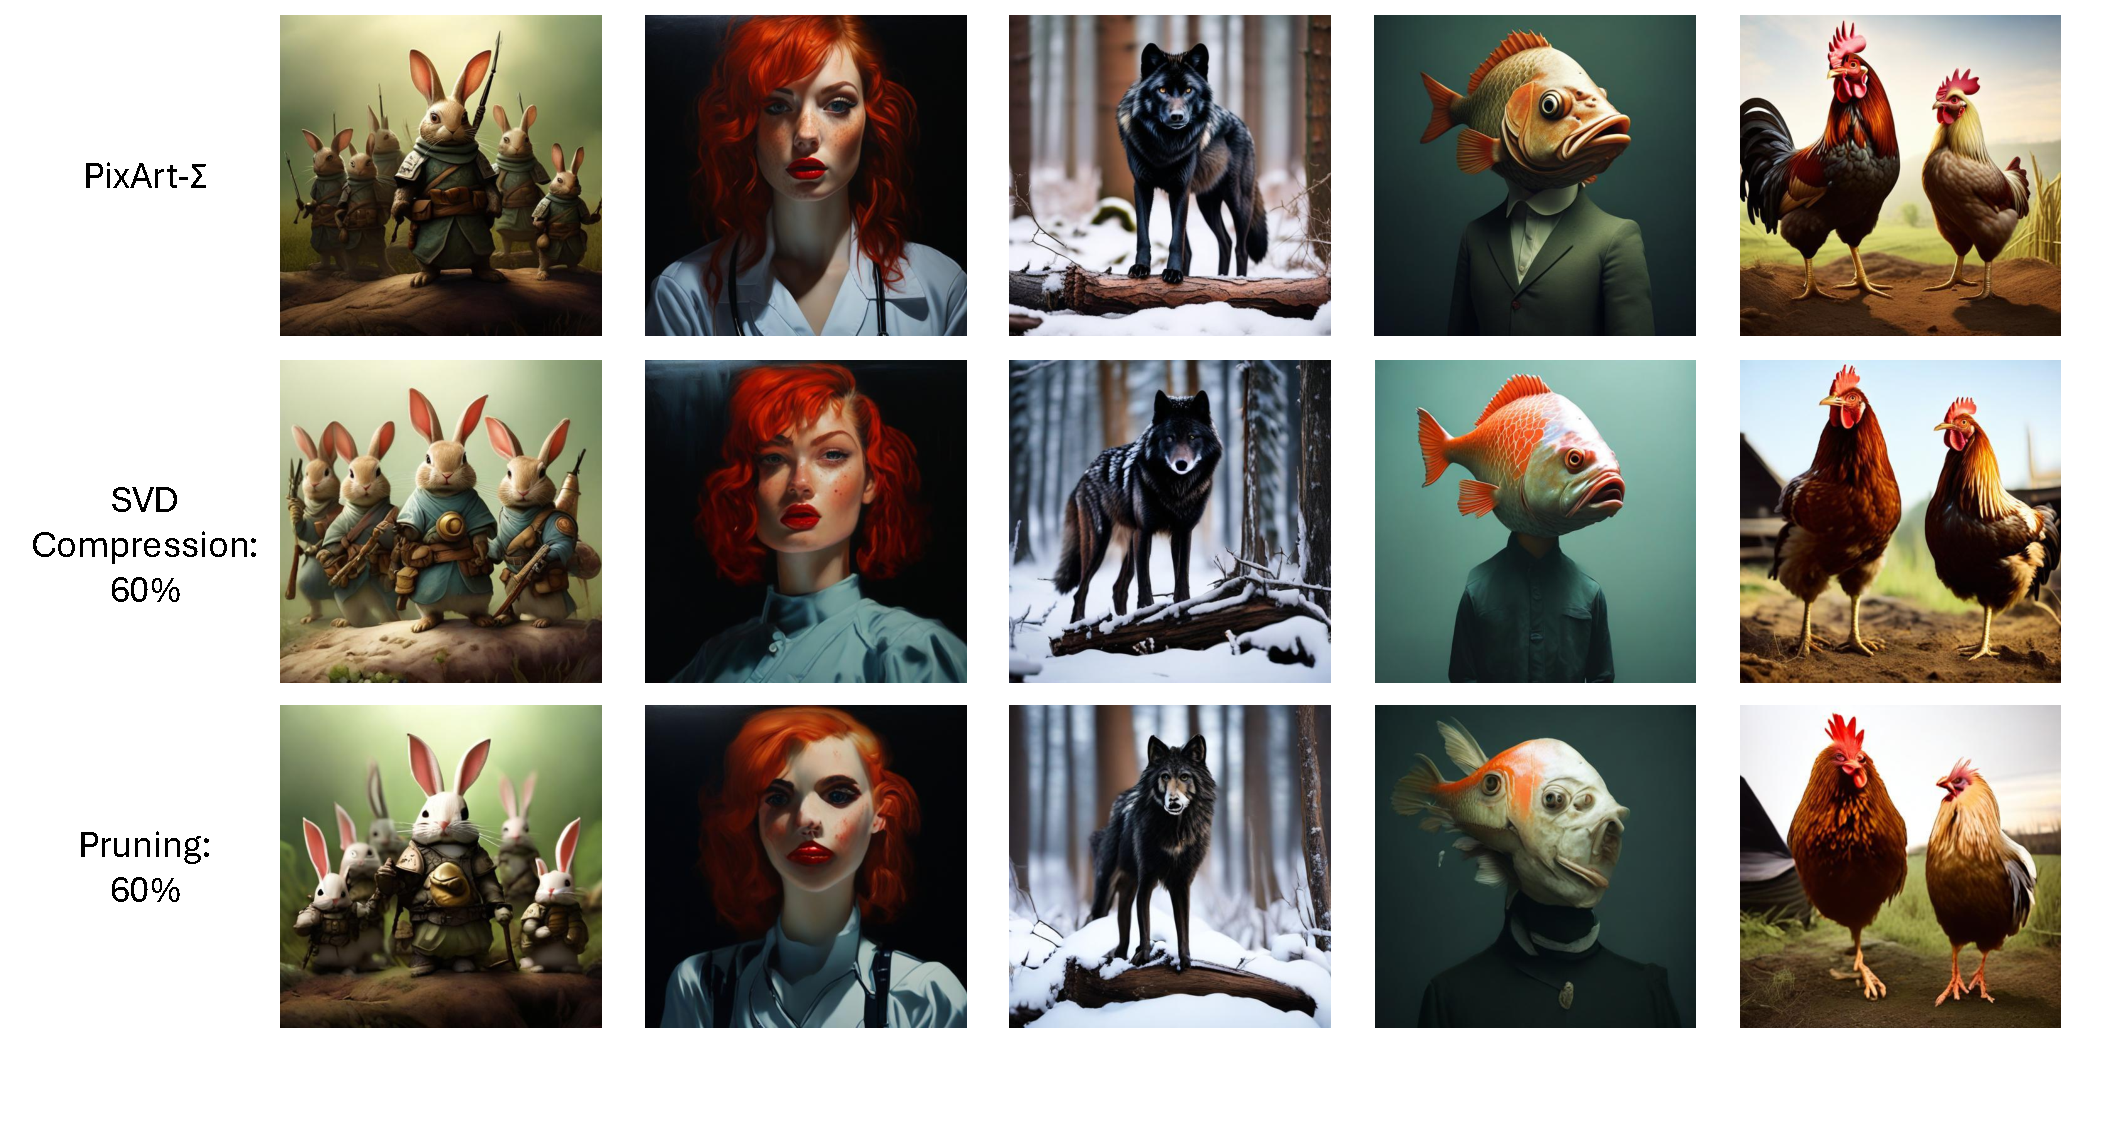
\includegraphics[width=0.9\textwidth]{images/Experimente/SVD_VS_Removal/ImageExamples_model60.pdf}
 	\caption[Qualitative Examples: Compression Strategies (60\% Pruning)]{Qualitative comparison of example images generated by models pruned to 60\% using complete block removal versus \gls{SVD}-based block compression.}
	\label{fig:Example_Images_SVD_vs_Removal_60_Appx}
\end{figure}



\section{Importance-Aware Rank-Adaptive Progressive Model Compression}
\label{appx:ImpAwRanAdProgComp}
Tab. \ref{tab:PixArtAppendixCompression_iterations} specifies the compression details for the experiments conducted in Sec. \ref{sec:CompressionSchedulingPixart}. Furthermore, qualitative examples for varying compression ratios are presented utilizing importance-aware rank-adaptive progressive model compression (Fig. \ref{fig:AppxCompressionSchedules90} - \ref{fig:AppxCompressionSchedules60}).
\begin{table}[H]
	\centering
\caption[Compression Details: Importance-Aware Rank-Adaptive Progressive Model Pruning]{Overview of the compression details utilized for the importance-aware rank-adaptive progressive model pruning experiments on the PixArt-$\Sigma$ model.}
	\label{tab:PixArtAppendixCompression_iterations}
	\begin{tabular}{ccccc}
		\toprule
		\textbf{Iteration} &\textbf{Model Size} & \textbf{Experiment} & \textbf{Base Compression Ratio} & \textbf{Slope} $x$\\
		\midrule
		\multirow{3}{*}{1} 
		& \multirow{3}{*}{90\%}  
		& \textbf{SVD\_7} & 0.6 & 0.0429 \\
		&  &   \textbf{SVD\_14} & 0.4 & 0.0083 \\
		&  &  \textbf{SVD\_21}  & 0.2 & 0.0043
		 \\
		\midrule
		\multirow{3}{*}{2} 
		& \multirow{3}{*}{80\%} 
		& \textbf{SVD\_7} & 0.6 & 0.0187 \\
		&  &    \textbf{SVD\_14} & 0.4 & 0.0059 \\
		&  & \textbf{SVD\_21}  & 0.2 & 0.0016
		 \\
		\midrule
		\multirow{3}{*}{3} 
		& \multirow{3}{*}{70\%}  
		& \textbf{SVD\_7} & 0.8 & 0.0364  \\
		&  &    \textbf{SVD\_14} & 0.6  & 0.0067 \\
		&  & \textbf{SVD\_21}  & 0.4 & 0.018
		  \\
		\midrule
		\multirow{3}{*}{4} 
		& \multirow{3}{*}{60\%}  
		& \textbf{SVD\_7} & 0.8 & 0.0656 \\
		&  &    \textbf{SVD\_14} & 0.6  & 0.0068 \\
		&  & \textbf{SVD\_21}  & 0.4 & 0.013
		 \\
		\midrule
		\multirow{3}{*}{5} 
		& \multirow{3}{*}{50\%}  
		& \textbf{SVD\_7} & 0.8 & 0.0799  \\
		&  &    \textbf{SVD\_14} & 0.6 & 0.0049 \\
		&  & \textbf{SVD\_21}  & 0.4 & 0.0090  \\
		\bottomrule
		
	\end{tabular}
\end{table}


	\begin{figure}[H]
	\centering
	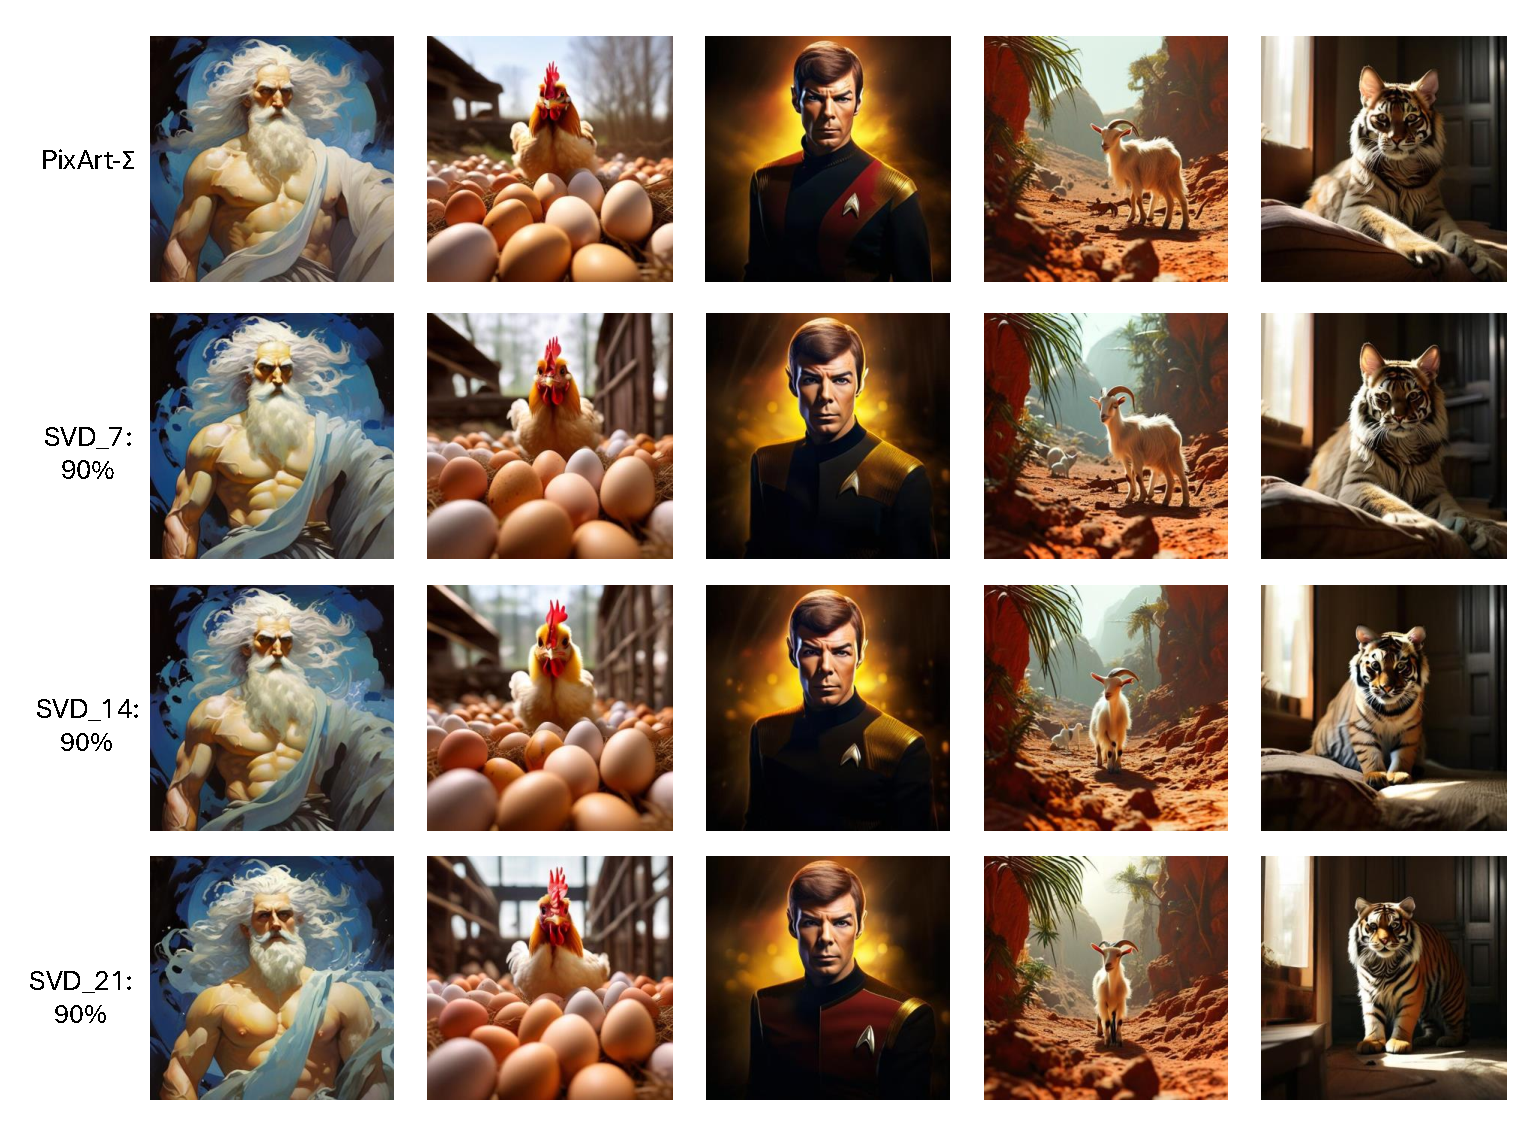
\includegraphics[width=0.7\textwidth]{images/Experimente/Compression_Schedul/ParameterDistribution_Appendix_model90.pdf}
 \caption[Qualitative Examples: Importance-Aware Rank-Adaptive Progressive Pruning (90\% Pruning)]{Qualitative comparison of example images generated by models pruned to 90\% using the importance-aware rank-adaptive progressive pruning schedule versus standard progressive pruning (last row). The rows illustrate experiments utilizing a varying number of blocks that are compressed per iteration.}
	\label{fig:AppxCompressionSchedules90}
\end{figure}

	\begin{figure}[H]
	\centering
	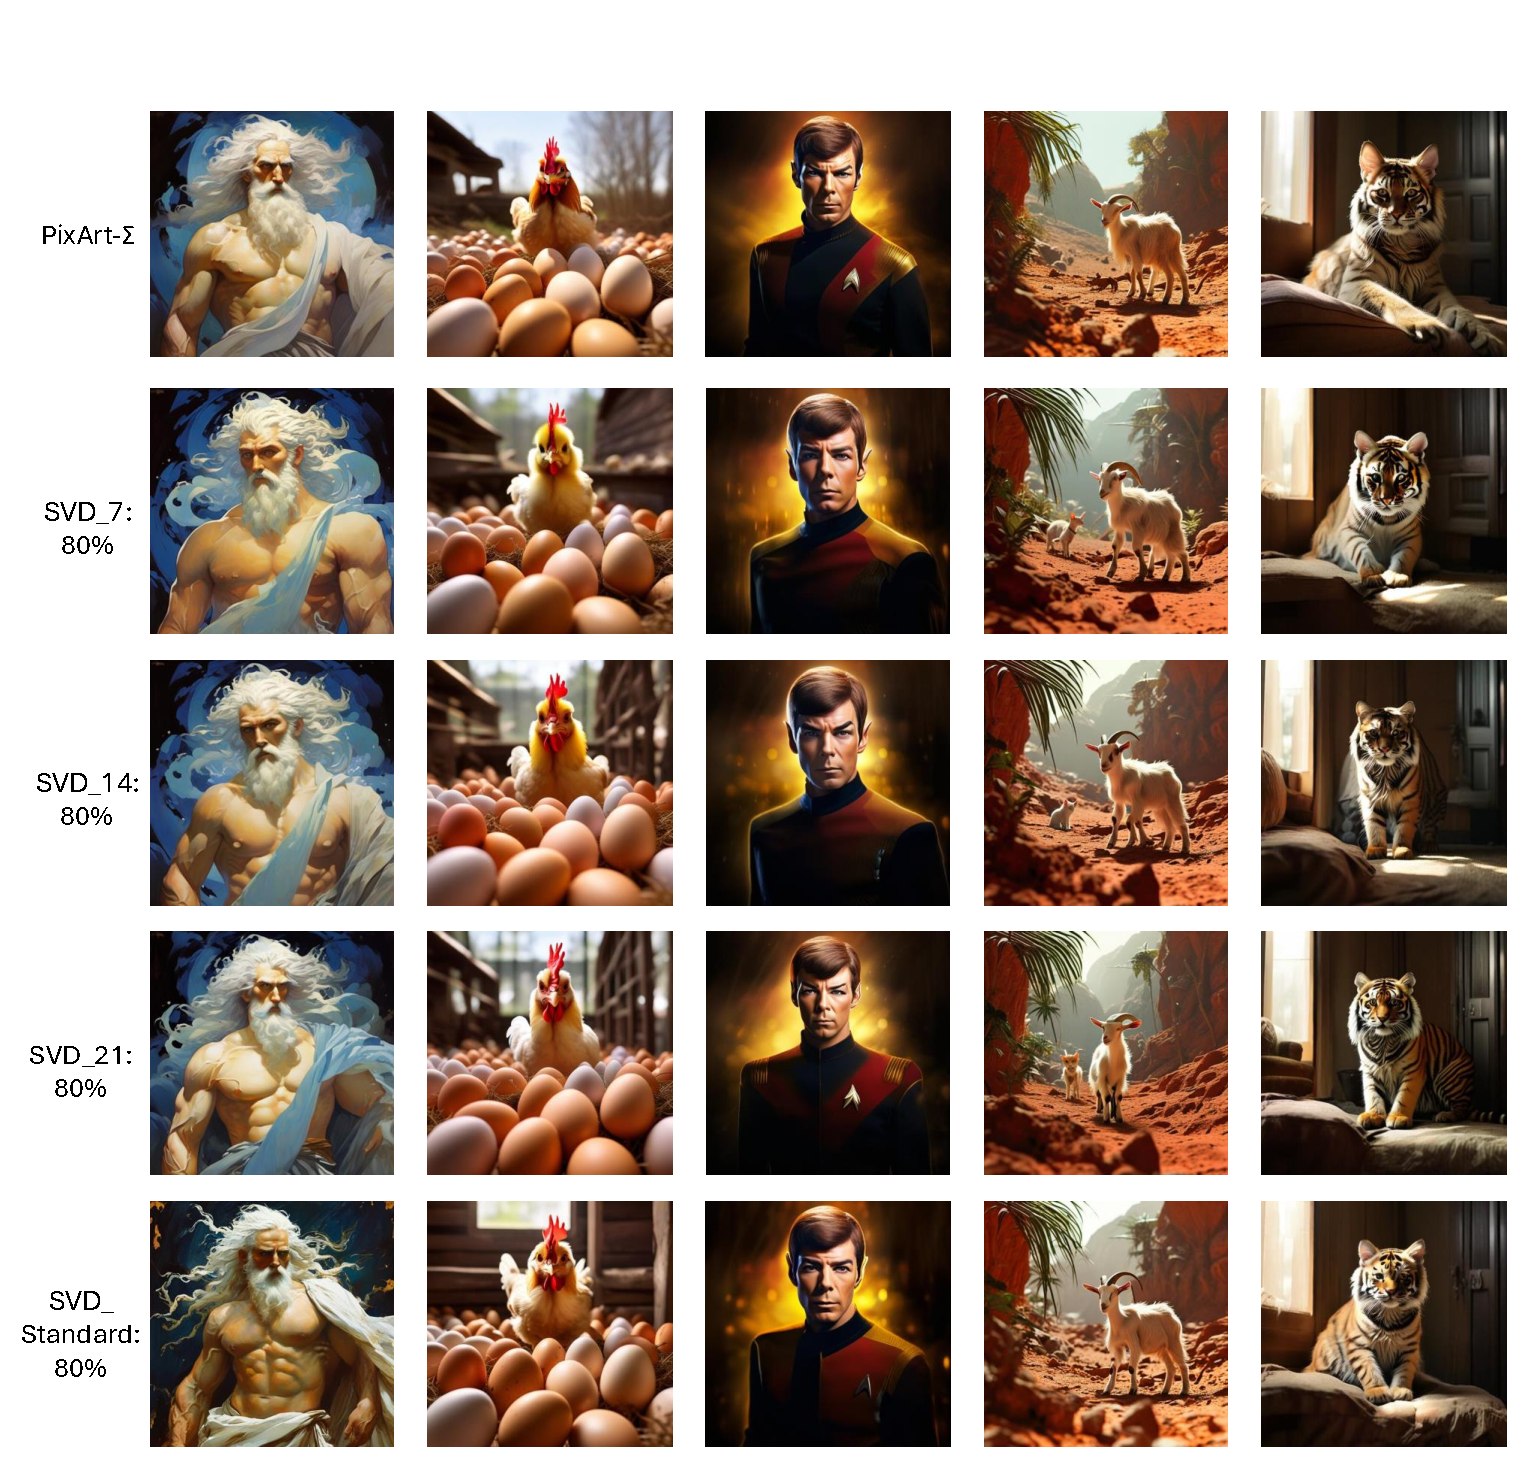
\includegraphics[width=0.7\textwidth]{images/Experimente/Compression_Schedul/ParameterDistribution_Appendix_model80.pdf}
 \caption[Qualitative Examples: Importance-Aware Rank-Adaptive Progressive Pruning (80\% Pruning)]{Qualitative comparison of example images generated by models pruned to 80\% using the importance-aware rank-adaptive progressive pruning schedule versus standard progressive pruning (last row). The rows illustrate experiments utilizing a varying number of blocks that are compressed per iteration.}
	\label{fig:AppxCompressionSchedules80}
\end{figure}


	\begin{figure}[H]
	\centering
	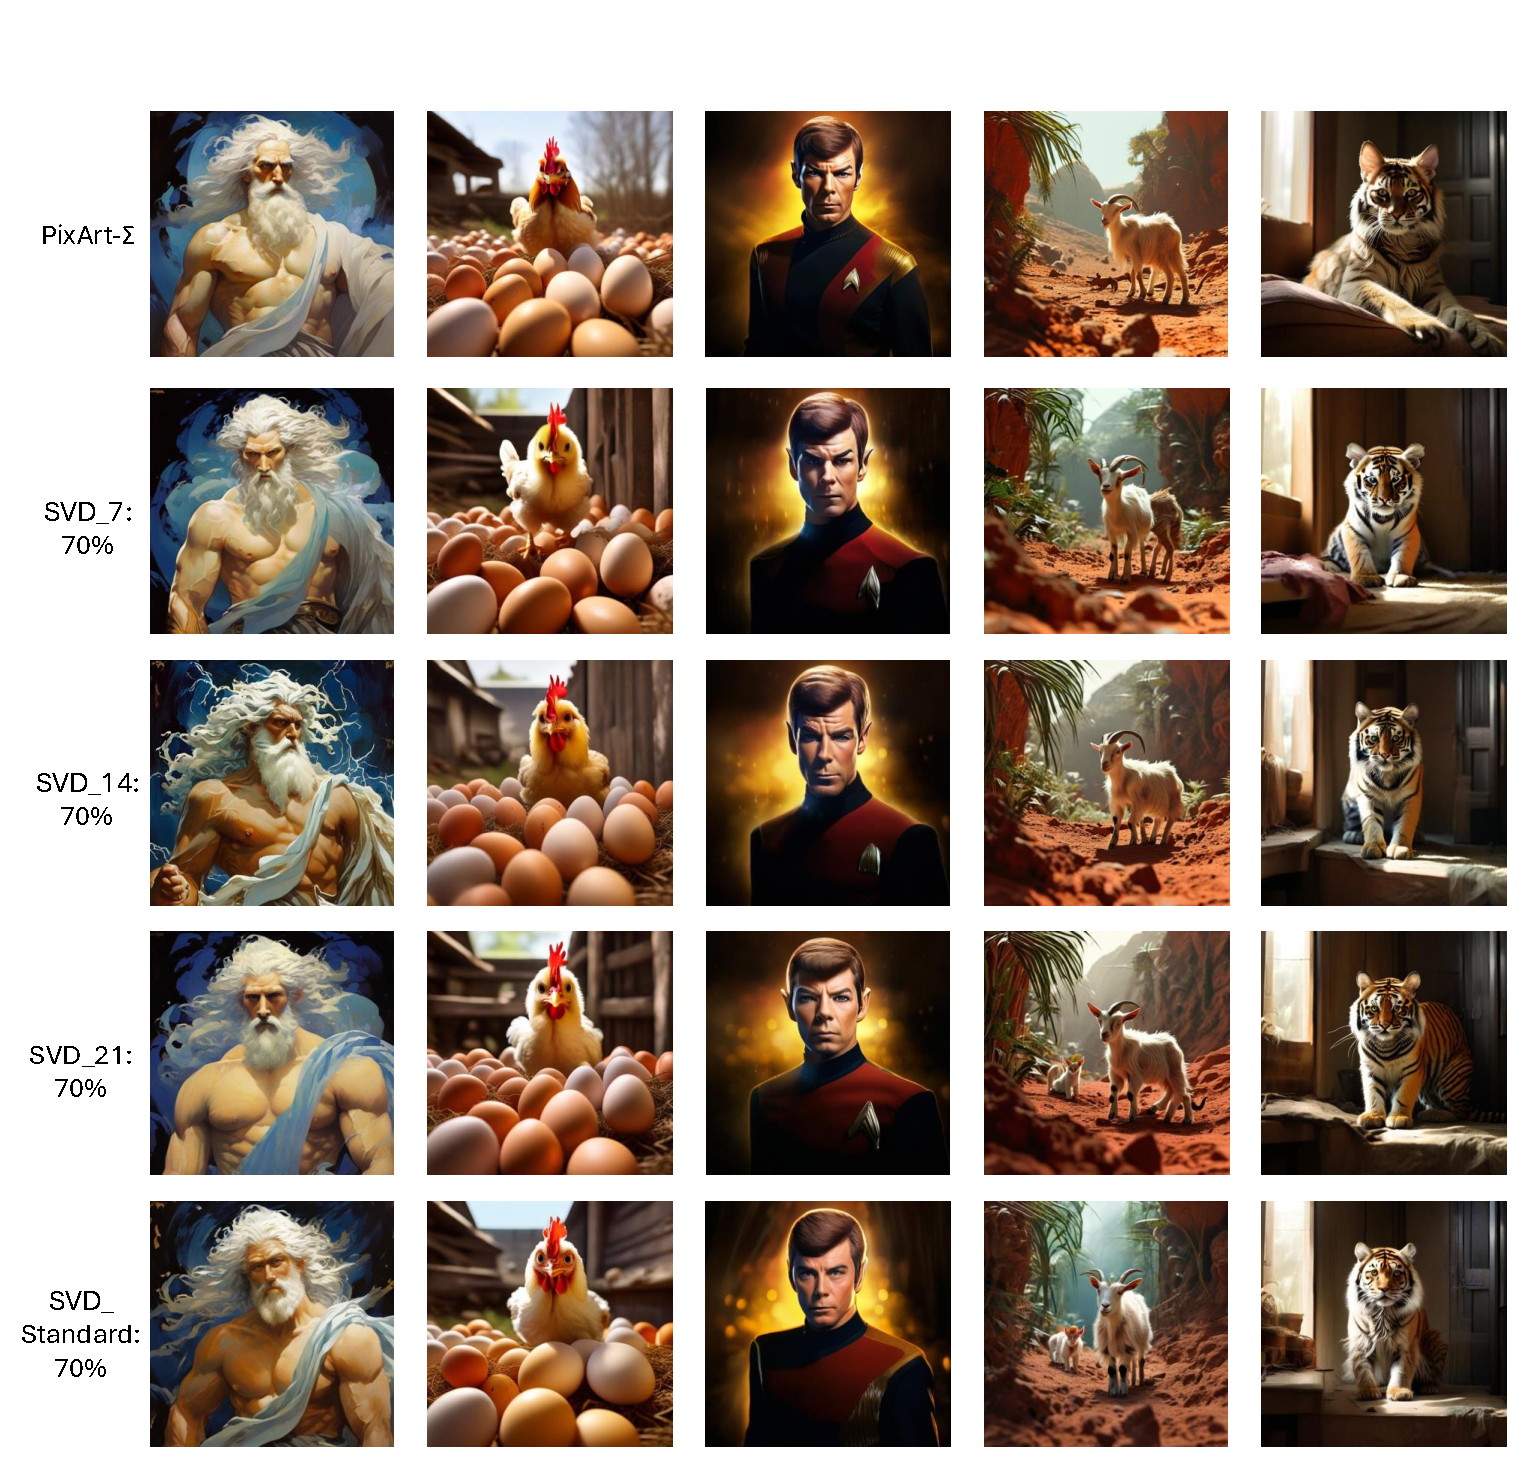
\includegraphics[width=0.7\textwidth]{images/Experimente/Compression_Schedul/ParameterDistribution_Appendix_model70.pdf}
 \caption[Qualitative Examples: Importance-Aware Rank-Adaptive Progressive Pruning (70\% Pruning)]{Qualitative comparison of example images generated by models pruned to 70\% using the importance-aware rank-adaptive progressive pruning schedule versus standard progressive pruning (last row). The rows illustrate experiments utilizing a varying number of blocks that are compressed per iteration.}
	\label{fig:AppxCompressionSchedules70}
\end{figure}


	\begin{figure}[H]
	\centering
	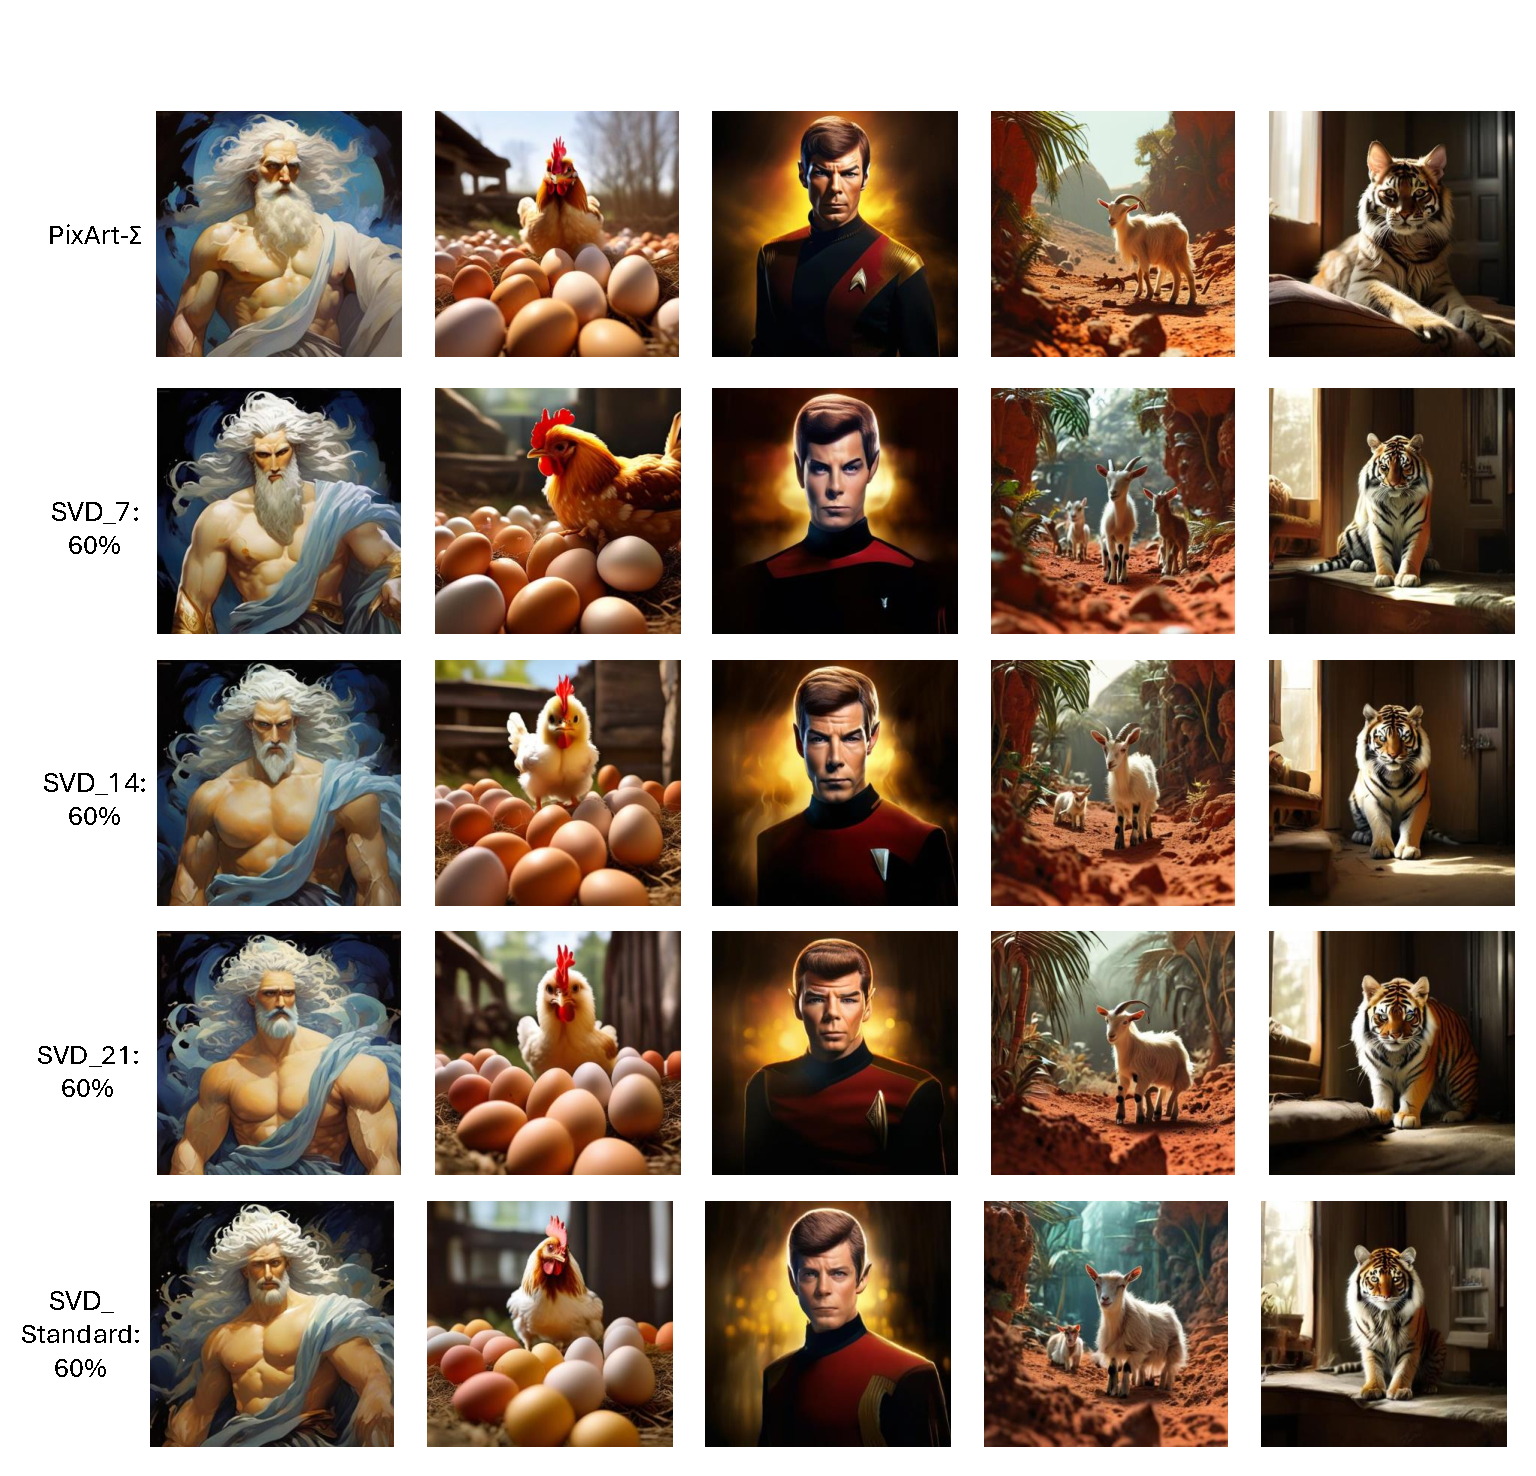
\includegraphics[width=0.7\textwidth]{images/Experimente/Compression_Schedul/ParameterDistribution_Appendix_model60.pdf}
 \caption[Qualitative Examples: Importance-Aware Rank-Adaptive Progressive Pruning (60\% Pruning)]{Qualitative comparison of example images generated by models pruned to 60\% using the importance-aware rank-adaptive progressive pruning schedule versus standard progressive pruning (last row). The rows illustrate experiments utilizing a varying number of blocks that are compressed per iteration.}
	\label{fig:AppxCompressionSchedules60}
\end{figure}




%\section{Detailed Overview of Selected Blocks Experiments PixArt-$\Sigma$}
%In this section, the removed or compressed blocks for each experiments are visualized. Different colors indicates during which iteration of the progressive pruning framework the specific block was selected. 


%\subsection{One-Shot vs. Progressive Blockverteilung}
%\label{sec:OneShotVsProgressive}
%
%% --- BILD 1: One-Shot vs Progressive 90% ---
%\begin{figure}[htbp]
%	\centering
%	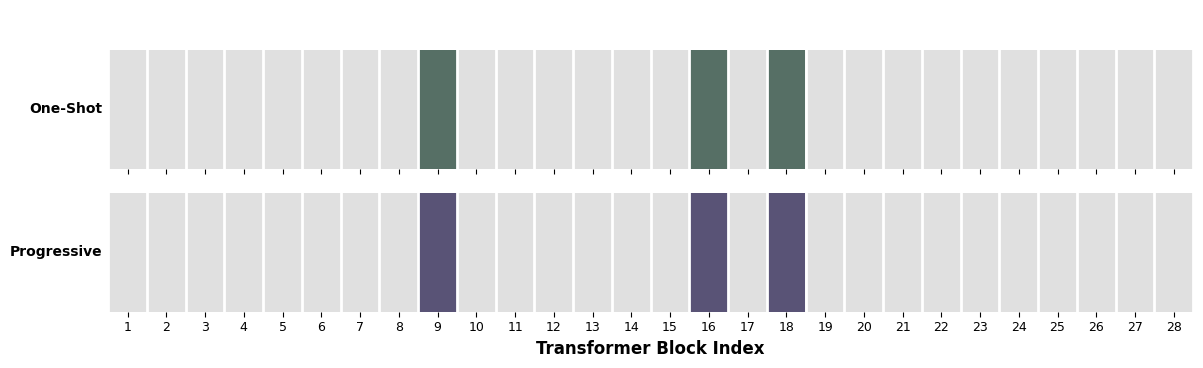
\includegraphics[width=0.9\textwidth]{images/Experimente/Block_Selection/OneShotvsIterative/model_90.png}
%	\caption{Comparison block selection for one-shot versus progressive pruning (90\% Parameter).}
%	\label{fig:OneShot_90}
%\end{figure}
%
%% --- BILD 2: One-Shot vs Progressive 80% ---
%\begin{figure}[htbp]
%	\centering
%	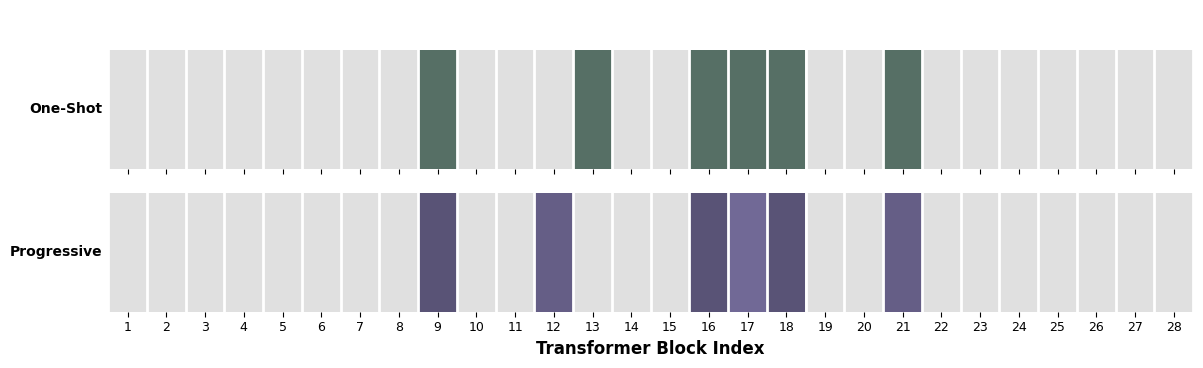
\includegraphics[width=0.9\textwidth]{images/Experimente/Block_Selection/OneShotvsIterative/model_80.png}
%	\caption{Comparison block selection for one-shot versus progressive pruning (80\% Parameter).}
%	\label{fig:OneShot_80}
%\end{figure}
%
%% --- BILD 3: One-Shot vs Progressive 70% ---
%\begin{figure}[htbp]
%	\centering
%	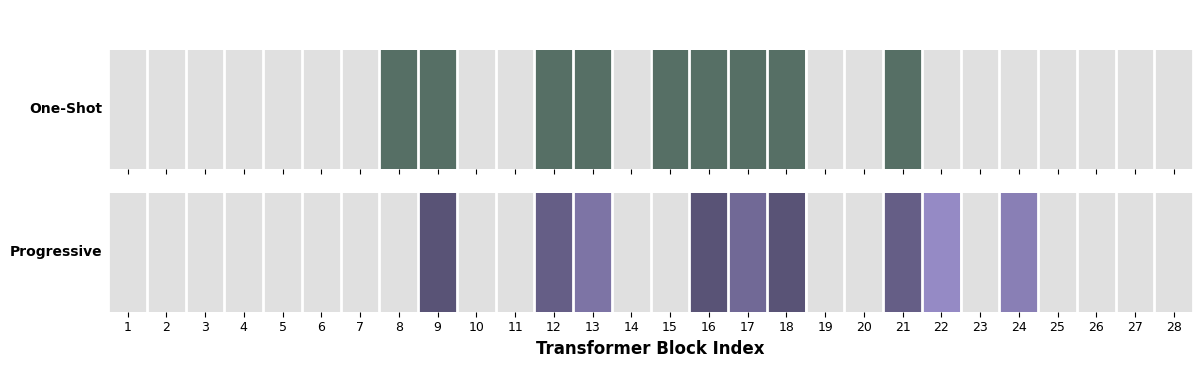
\includegraphics[width=0.9\textwidth]{images/Experimente/Block_Selection/OneShotvsIterative/model_70.png}
%	\caption{Comparison block selection for one-shot versus progressive pruning (70\% Parameter).}
%	\label{fig:OneShot_70}
%\end{figure}
%
%% --- BILD 4: One-Shot vs Progressive 60% ---
%\begin{figure}[htbp]
%	\centering
%	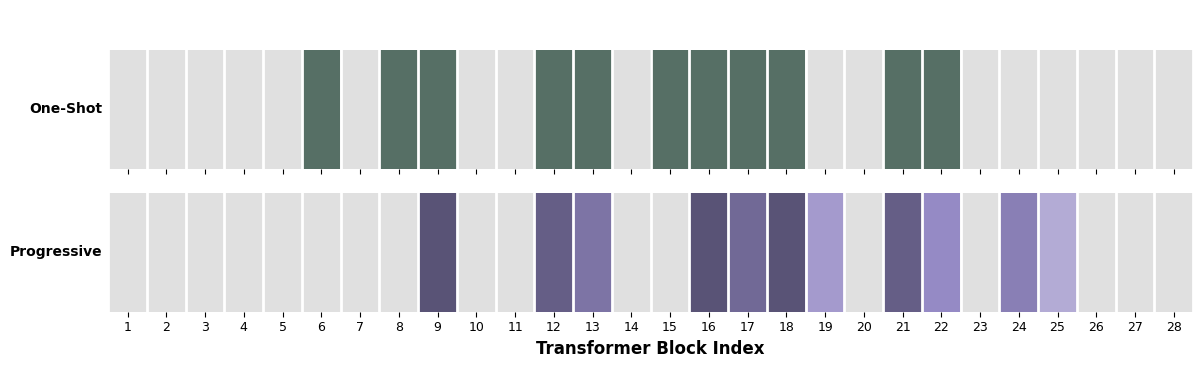
\includegraphics[width=0.9\textwidth]{images/Experimente/Block_Selection/OneShotvsIterative/model_60.png}
%	\caption{Comparison block selection for one-shot versus progressive pruning (60\% Parameter).}
%	\label{fig:OneShot_60}
%\end{figure}
%
%% --- BILD 5: One-Shot vs Progressive 50% ---
%\begin{figure}[htbp]
%	\centering
%	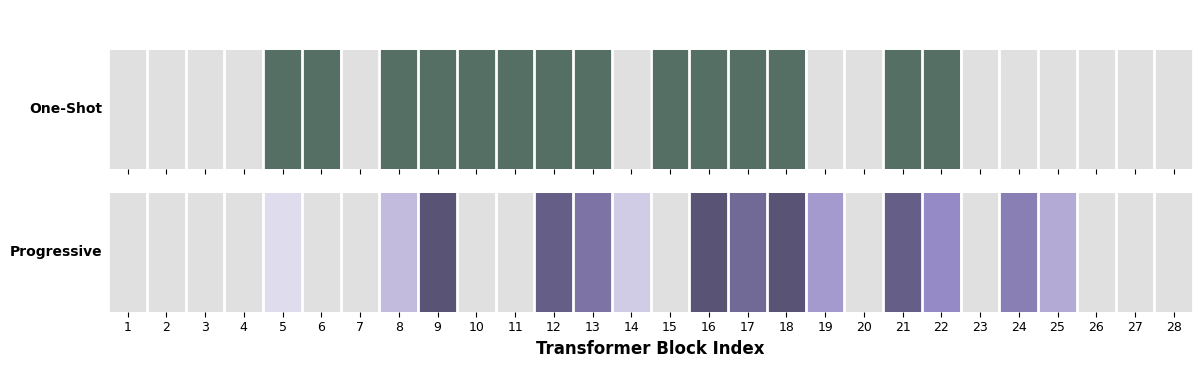
\includegraphics[width=0.9\textwidth]{images/Experimente/Block_Selection/OneShotvsIterative/model_50.png}
%	\caption{Comparison block selection for one-shot versus progressive pruning (50\% Parameter).}
%	\label{fig:OneShot_50}
%\end{figure}
%
%\clearpage % Optional: Erzwingt, dass alle bisherigen Bilder ausgegeben werden, bevor die nächste Sektion startet
%
%\subsection{Knowledge Distillation Loss}
%\label{sec:BlockSelection_LossInvestigation}
%
%% --- BILD 6: Loss Investigation 90% ---
%\begin{figure}[htbp]
%	\centering
%	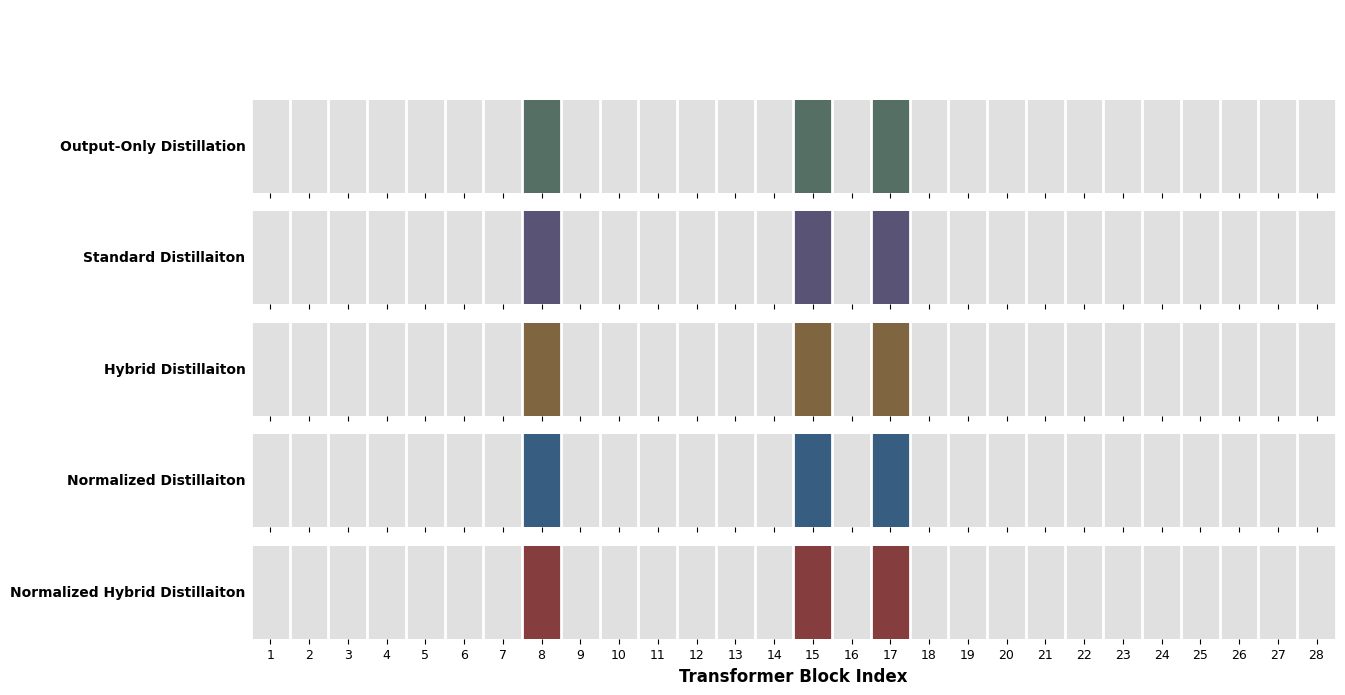
\includegraphics[width=0.9\textwidth]{images/Experimente/Block_Selection/Loss_Investigation/model_90.png}
%	\caption{Influence of the loss configuration for block selection (90\% Parameter).}
%	\label{fig:Loss_90}
%\end{figure}
%
%% --- BILD 7: Loss Investigation 80% ---
%\begin{figure}[htbp]
%	\centering
%	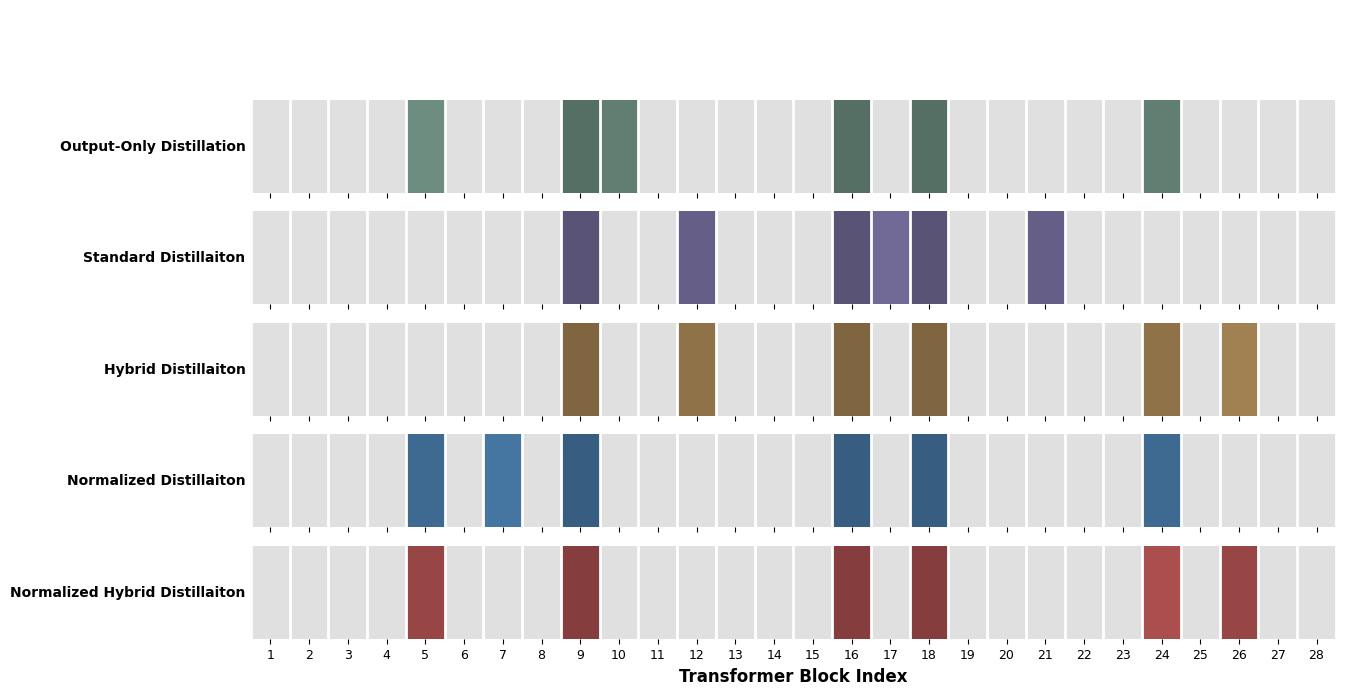
\includegraphics[width=0.9\textwidth]{images/Experimente/Block_Selection/Loss_Investigation/model_80.png}
%	\caption{Influence of the loss configuration for block selection (80\% Parameter).}
%	\label{fig:Loss_80}
%\end{figure}
%
%% --- BILD 8: Loss Investigation 70% ---
%\begin{figure}[htbp]
%	\centering
%	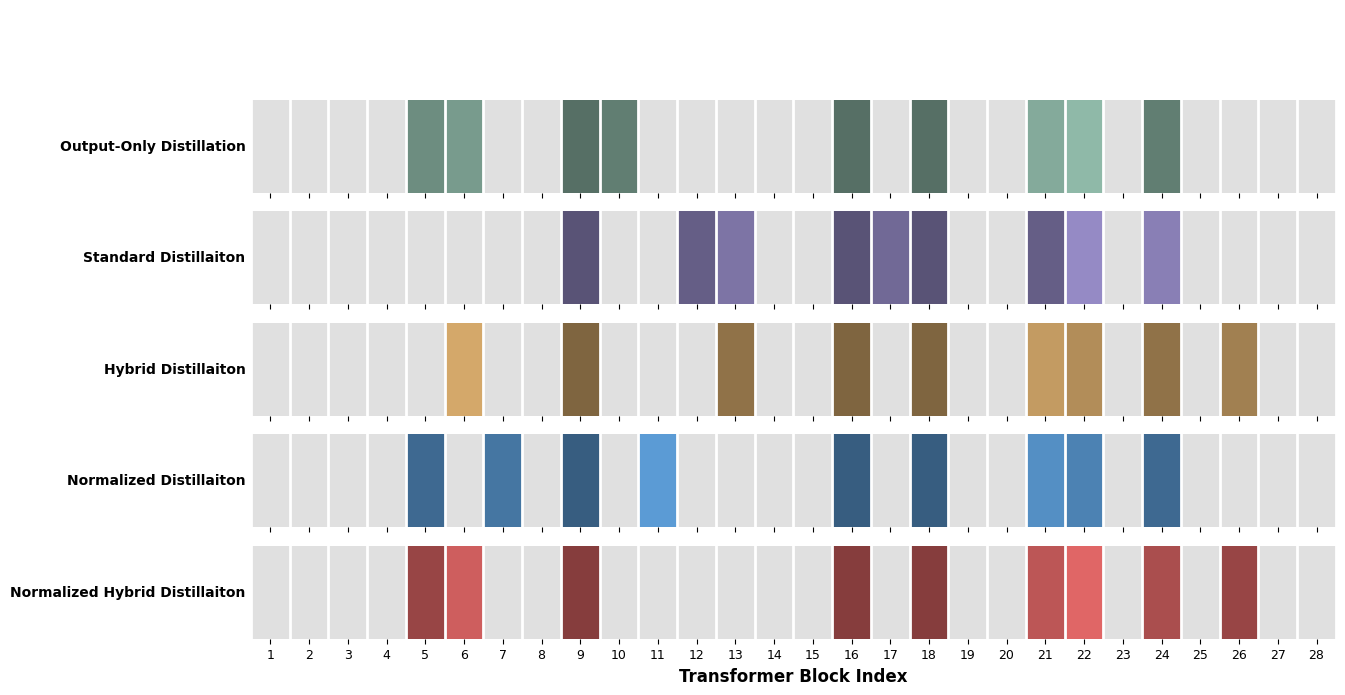
\includegraphics[width=0.9\textwidth]{images/Experimente/Block_Selection/Loss_Investigation/model_70.png}
%	\caption{Influence of the loss configuration for block selection (70\% Parameter).}
%	\label{fig:Loss_70}
%\end{figure}
%
%% --- BILD 9: Loss Investigation 60% ---
%\begin{figure}[htbp]
%	\centering
%	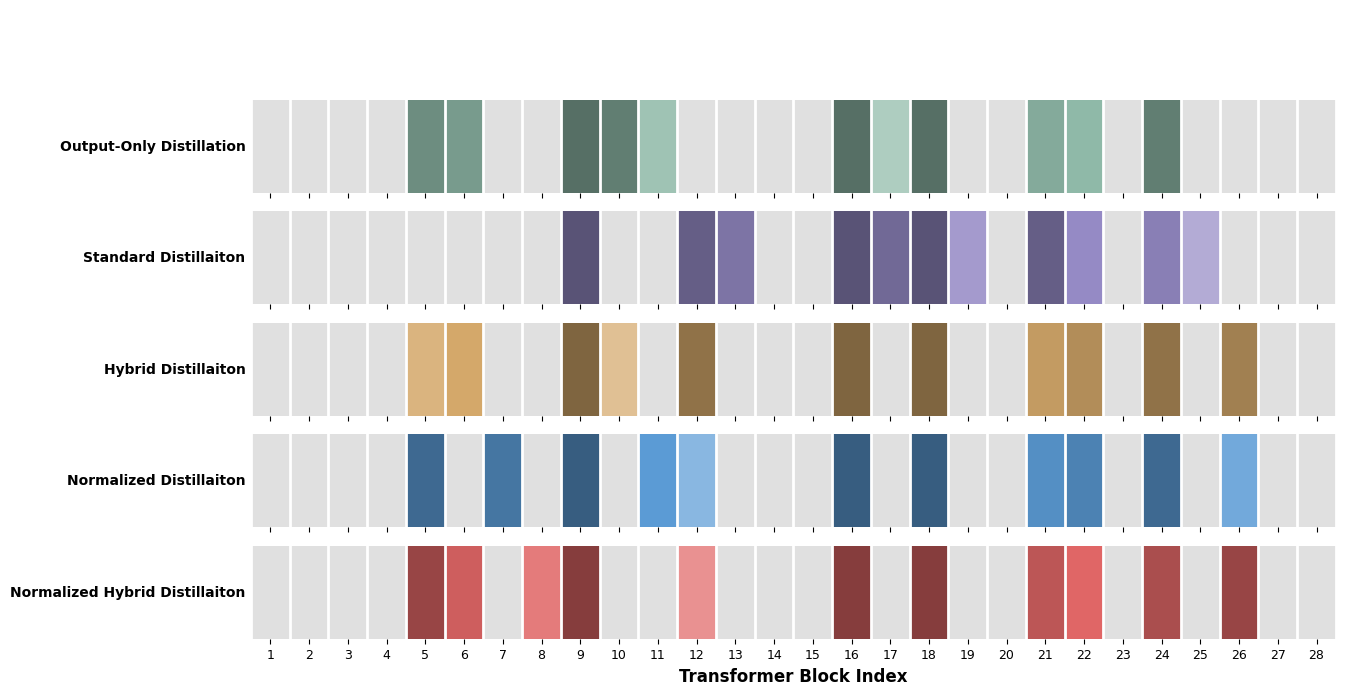
\includegraphics[width=0.9\textwidth]{images/Experimente/Block_Selection/Loss_Investigation/model_60.png}
%	\caption{Influence of the loss configuration for block selection (60\% Parameter).}
%	\label{fig:Loss_60}
%\end{figure}
%
%% --- BILD 10: Loss Investigation 50% ---
%\begin{figure}[htbp]
%	\centering
%	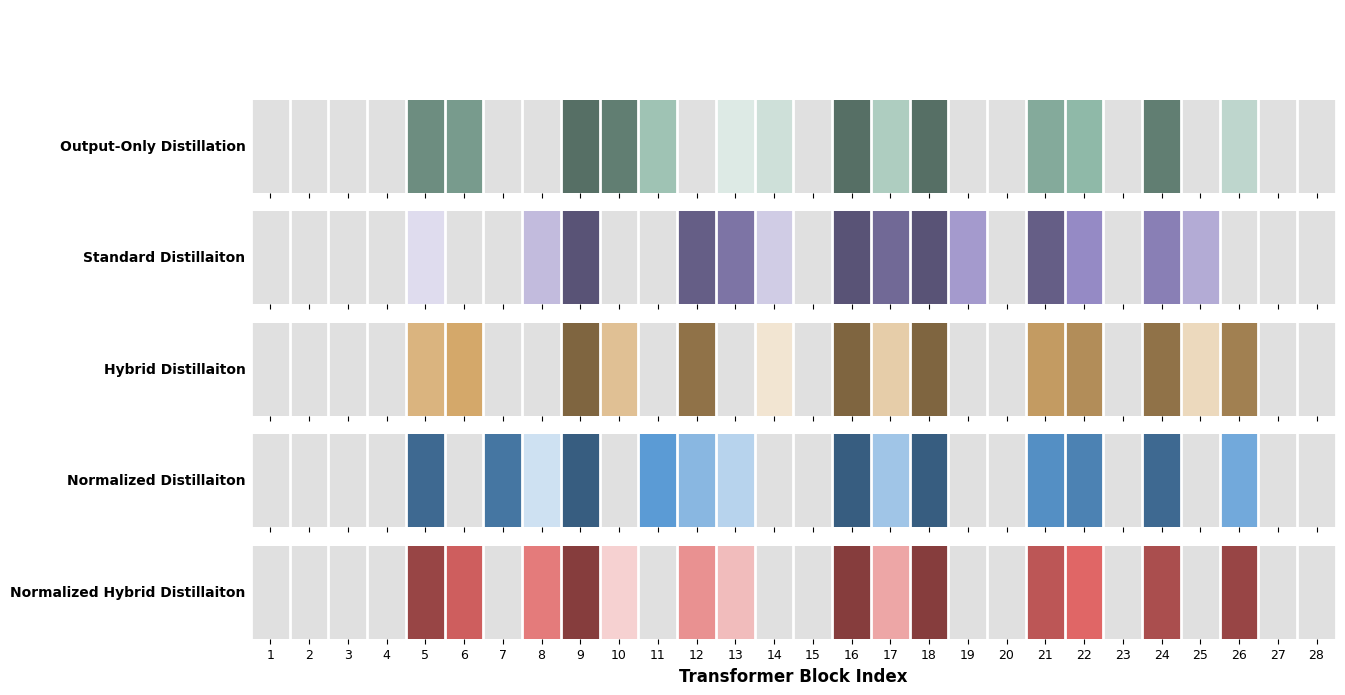
\includegraphics[width=0.9\textwidth]{images/Experimente/Block_Selection/Loss_Investigation/model_50.png}
%	\caption{Influence of the loss configuration for block selectionn (50\% Parameter).}
%	\label{fig:Loss_50}
%\end{figure}
%
%
%
%\subsection{Finetuning Protocol}
%\label{sec:BlockSelection_FinetuningProtocol}
%
%% --- BILD 6: Loss Investigation 90% ---
%\begin{figure}[H]
%	\centering
%	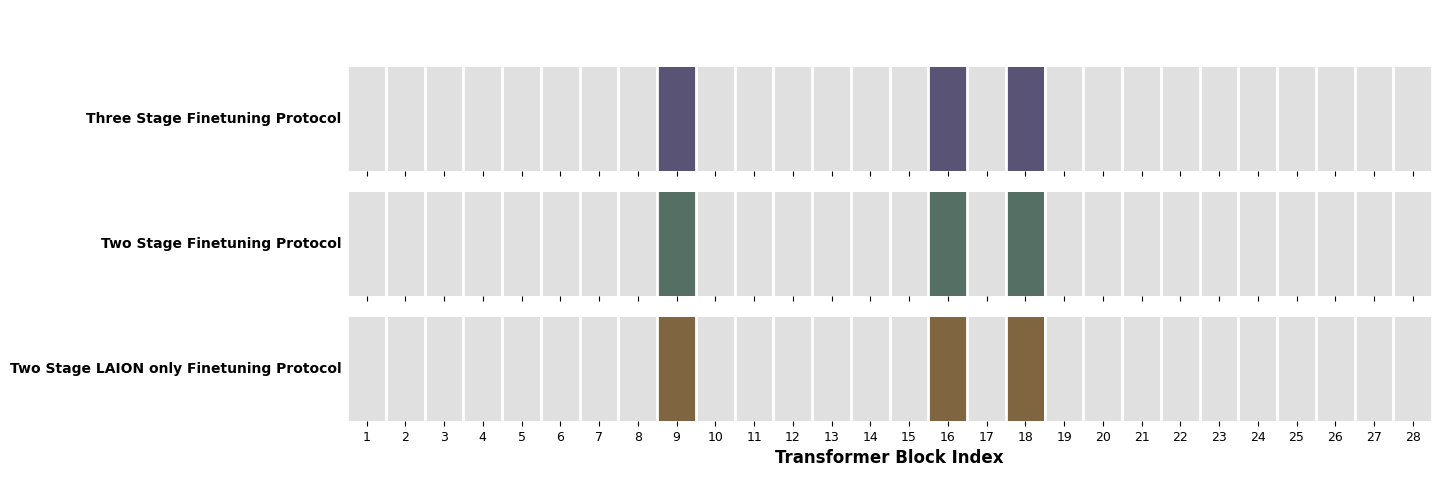
\includegraphics[width=0.9\textwidth]{images/Experimente/Block_Selection/Finetuning_Protocol/model_90.png}
%	\caption{Influence of the finetuning protocol for block selection (90\% Parameter).}
%	\label{fig:Loss_90}
%\end{figure}
%
%% --- BILD 7: Loss Investigation 80% ---
%\begin{figure}[htbp]
%	\centering
%	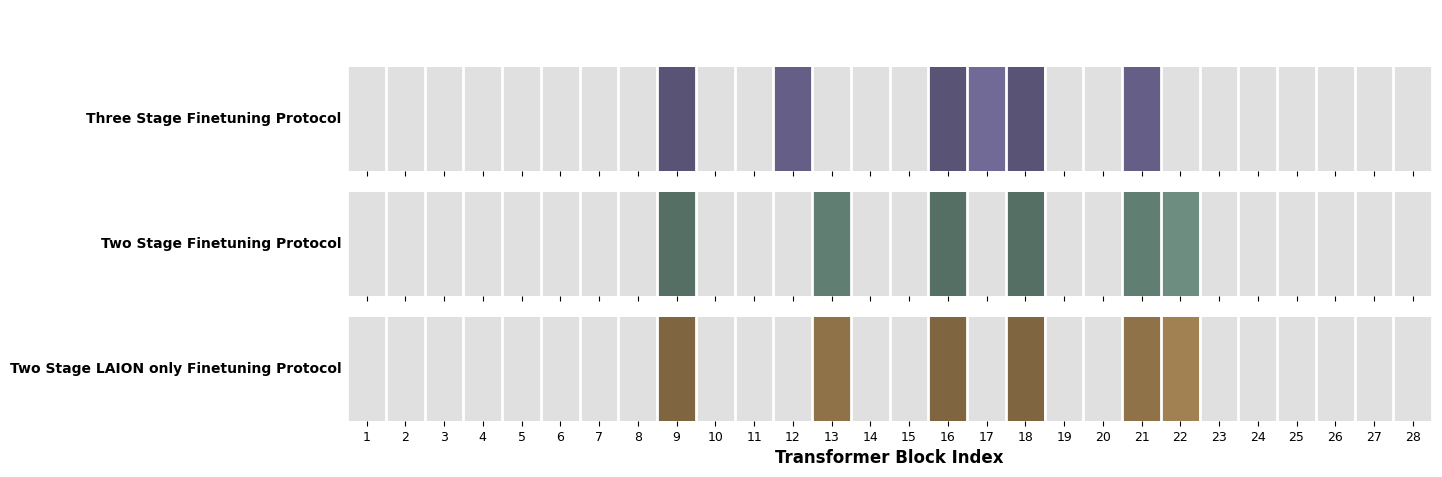
\includegraphics[width=0.9\textwidth]{images/Experimente/Block_Selection/Finetuning_Protocol/model_80.png}
%	\caption{Influence of the finetuning protocol for block selection (80\% Parameter).}
%	\label{fig:Loss_80}
%\end{figure}
%
%% --- BILD 8: Loss Investigation 70% ---
%\begin{figure}[htbp]
%	\centering
%	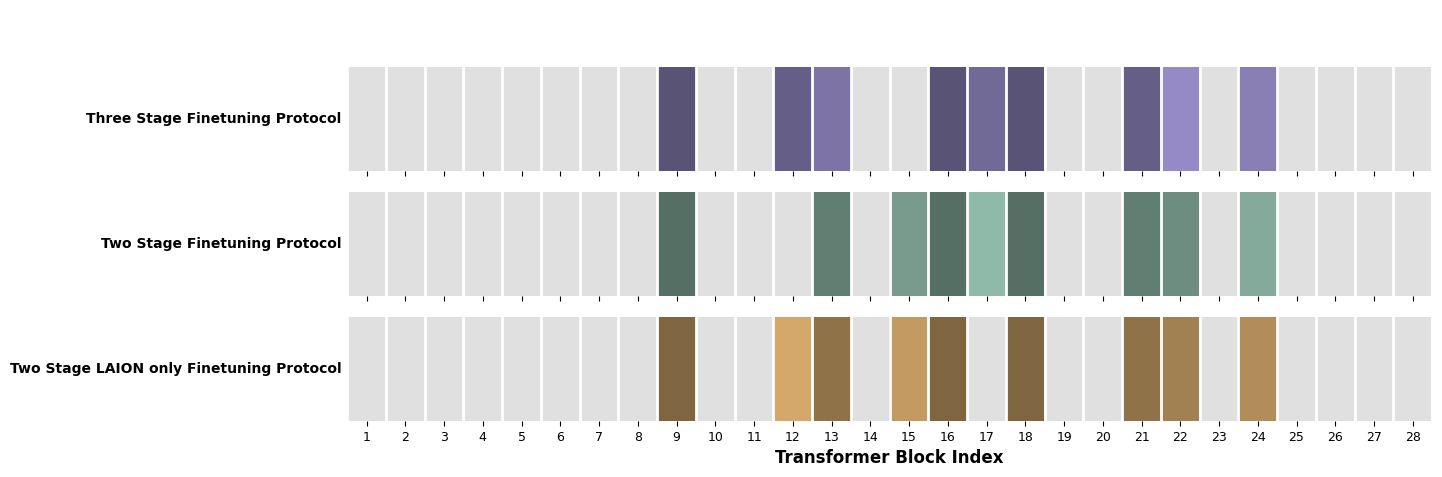
\includegraphics[width=0.9\textwidth]{images/Experimente/Block_Selection/Finetuning_Protocol/model_70.png}
%	\caption{Influence of the finetuning protocol for block selection (70\% Parameter).}
%	\label{fig:Loss_70}
%\end{figure}
%
%% --- BILD 9: Loss Investigation 60% ---
%\begin{figure}[htbp]
%	\centering
%	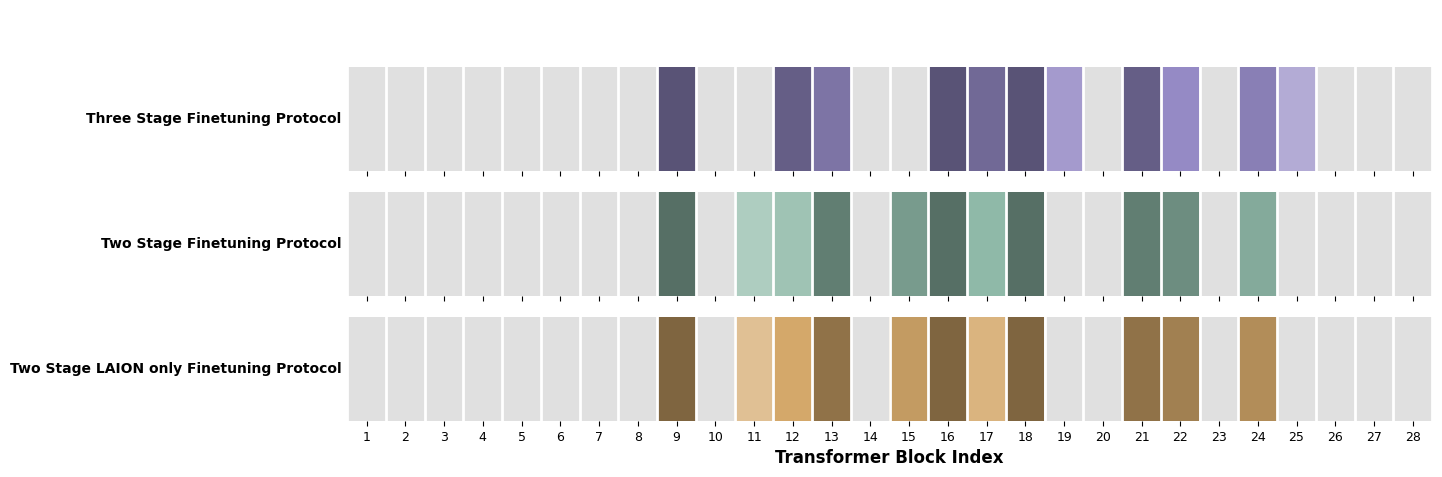
\includegraphics[width=0.9\textwidth]{images/Experimente/Block_Selection/Finetuning_Protocol/model_60.png}
%	\caption{Influence of the finetuning protocol for block selection (60\% Parameter).}
%	\label{fig:Loss_60}
%\end{figure}
%
%% --- BILD 10: Loss Investigation 50% ---
%\begin{figure}[htbp]
%	\centering
%	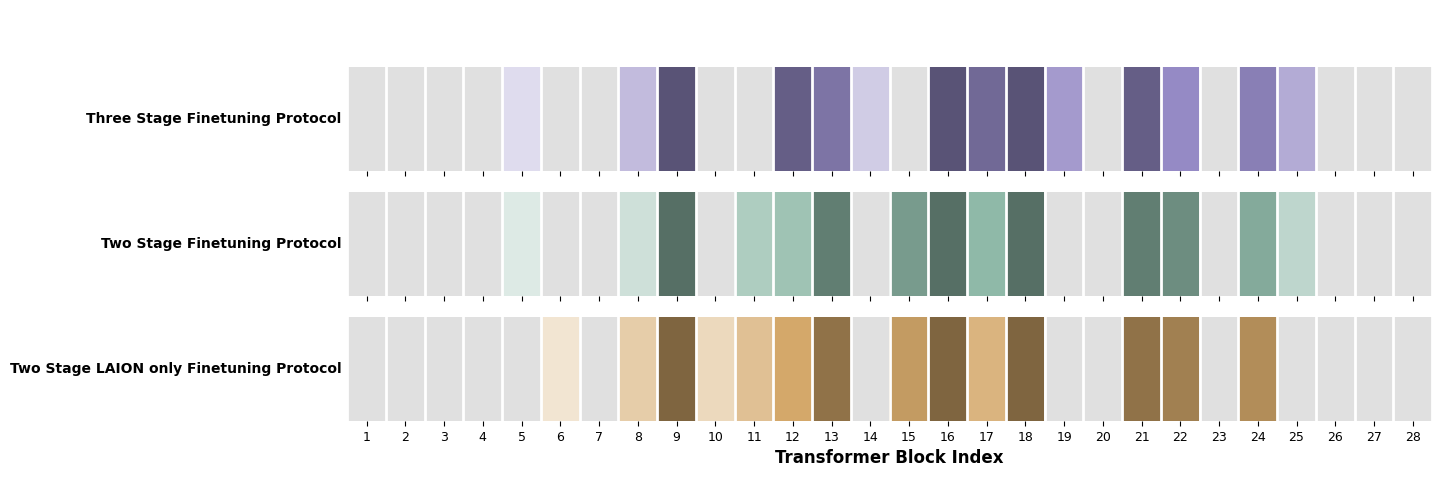
\includegraphics[width=0.9\textwidth]{images/Experimente/Block_Selection/Finetuning_Protocol/model_50.png}
%	\caption{Influence of the finetuning protocol for block selection (50\% Parameter).}
%	\label{fig:Loss_50}
%\end{figure}


\chapter{SupplementsFlux.1-dev Experiments}

\section{Training Details}
\begin{table}[H]
	\centering
	\caption[Flux.1-dev Fine-Funing Hyperparameters]{Configuration details for the compressed model retraining, including optimizer settings and flow matching specific parameters. These parameters represent the configuration setup for the training using the git repository \cite{kohya_ss_sd_scripts_2024}.}
	\label{tab:flux_training_config}
	\begin{tabular}{l l}
		\toprule
		\textbf{Hyperparameter} & \textbf{Value} \\
		\midrule
		\multicolumn{2}{l}{\textit{\textbf{Optimization \& Scheduler}}} \\
		Optimizer Type & Adafactor \\
		Optimizer Arguments & \small{relative\_step=False, scale\_parameter=False, warmup\_init=False} \\
		Learning Rate & $1.8 \times 10^{-6}$ \\
		LR Scheduler & constant\_with\_warmup \\
		LR Warmup Steps & 4240 \\
		Gradient Accumulation & 4 \\
		Batch Size & 1 \\
		\midrule
		\multicolumn{2}{l}{\textit{\textbf{Model Precision \& Hardware}}} \\
		Mixed Precision & bf16 \\
		Weight Precision (Base) & fp8 \\
		Full bfloat16 Training & True \\
		Gradient Checkpointing & True \\
		SDPA (Scaled Dot Product Attn) & True \\
		GPU & 1 $\times$ H200 \\
		\midrule
		\multicolumn{2}{l}{\textit{\textbf{Flow Matching \& Loss Settings}}} \\
		Discrete Flow Shift & 3 \\
		Timestep Sampling & sigmoid \\
		Max Timestep & 1000 \\
		Loss Type & L2 \\
		Huber Parameter ($c$) & 0.1 \\
		Huber Schedule & snr \\
		Model Prediction Type & raw \\
		Guidance Scale & 1.0 \\
		Sample Sampler & euler\_a \\
		\midrule
		\multicolumn{2}{l}{\textit{\textbf{Architecture \& Data Settings}}} \\
		T5 Max Token Length & 512 \\
		Clip Skip & 1 \\
		Apply T5 Attn Mask & True \\
		Data Loader Workers & 6 \\
		Seed & 42 \\
		Training Dataset & LAION-Flux.1-dev\\
		Size Training Dataset & 190 000 \\
		\bottomrule
	\end{tabular}
\end{table}


\section{Block Importance Analysis}
\label{appx:FluxBlockImportanceAnalysis}
Fig. \ref{fig:AppxBlockAnalysisRemovalDouble} and Fig. \ref{fig:AppxBlockAnalysisRemovalSingle} present the complete set of qualitative examples of a generated images when one complete double- or single-stream block is removed. 

Fig. \ref{fig:AppxBlockAnalysisCompressionDouble} and Fig. \ref{fig:AppxBlockAnalysisCompressionSingle} present qualitative examples of a generated images when one complete double- or single-stream block is compressed via truncated \gls{SVD}. 


\begin{figure}[H]
	\centering
	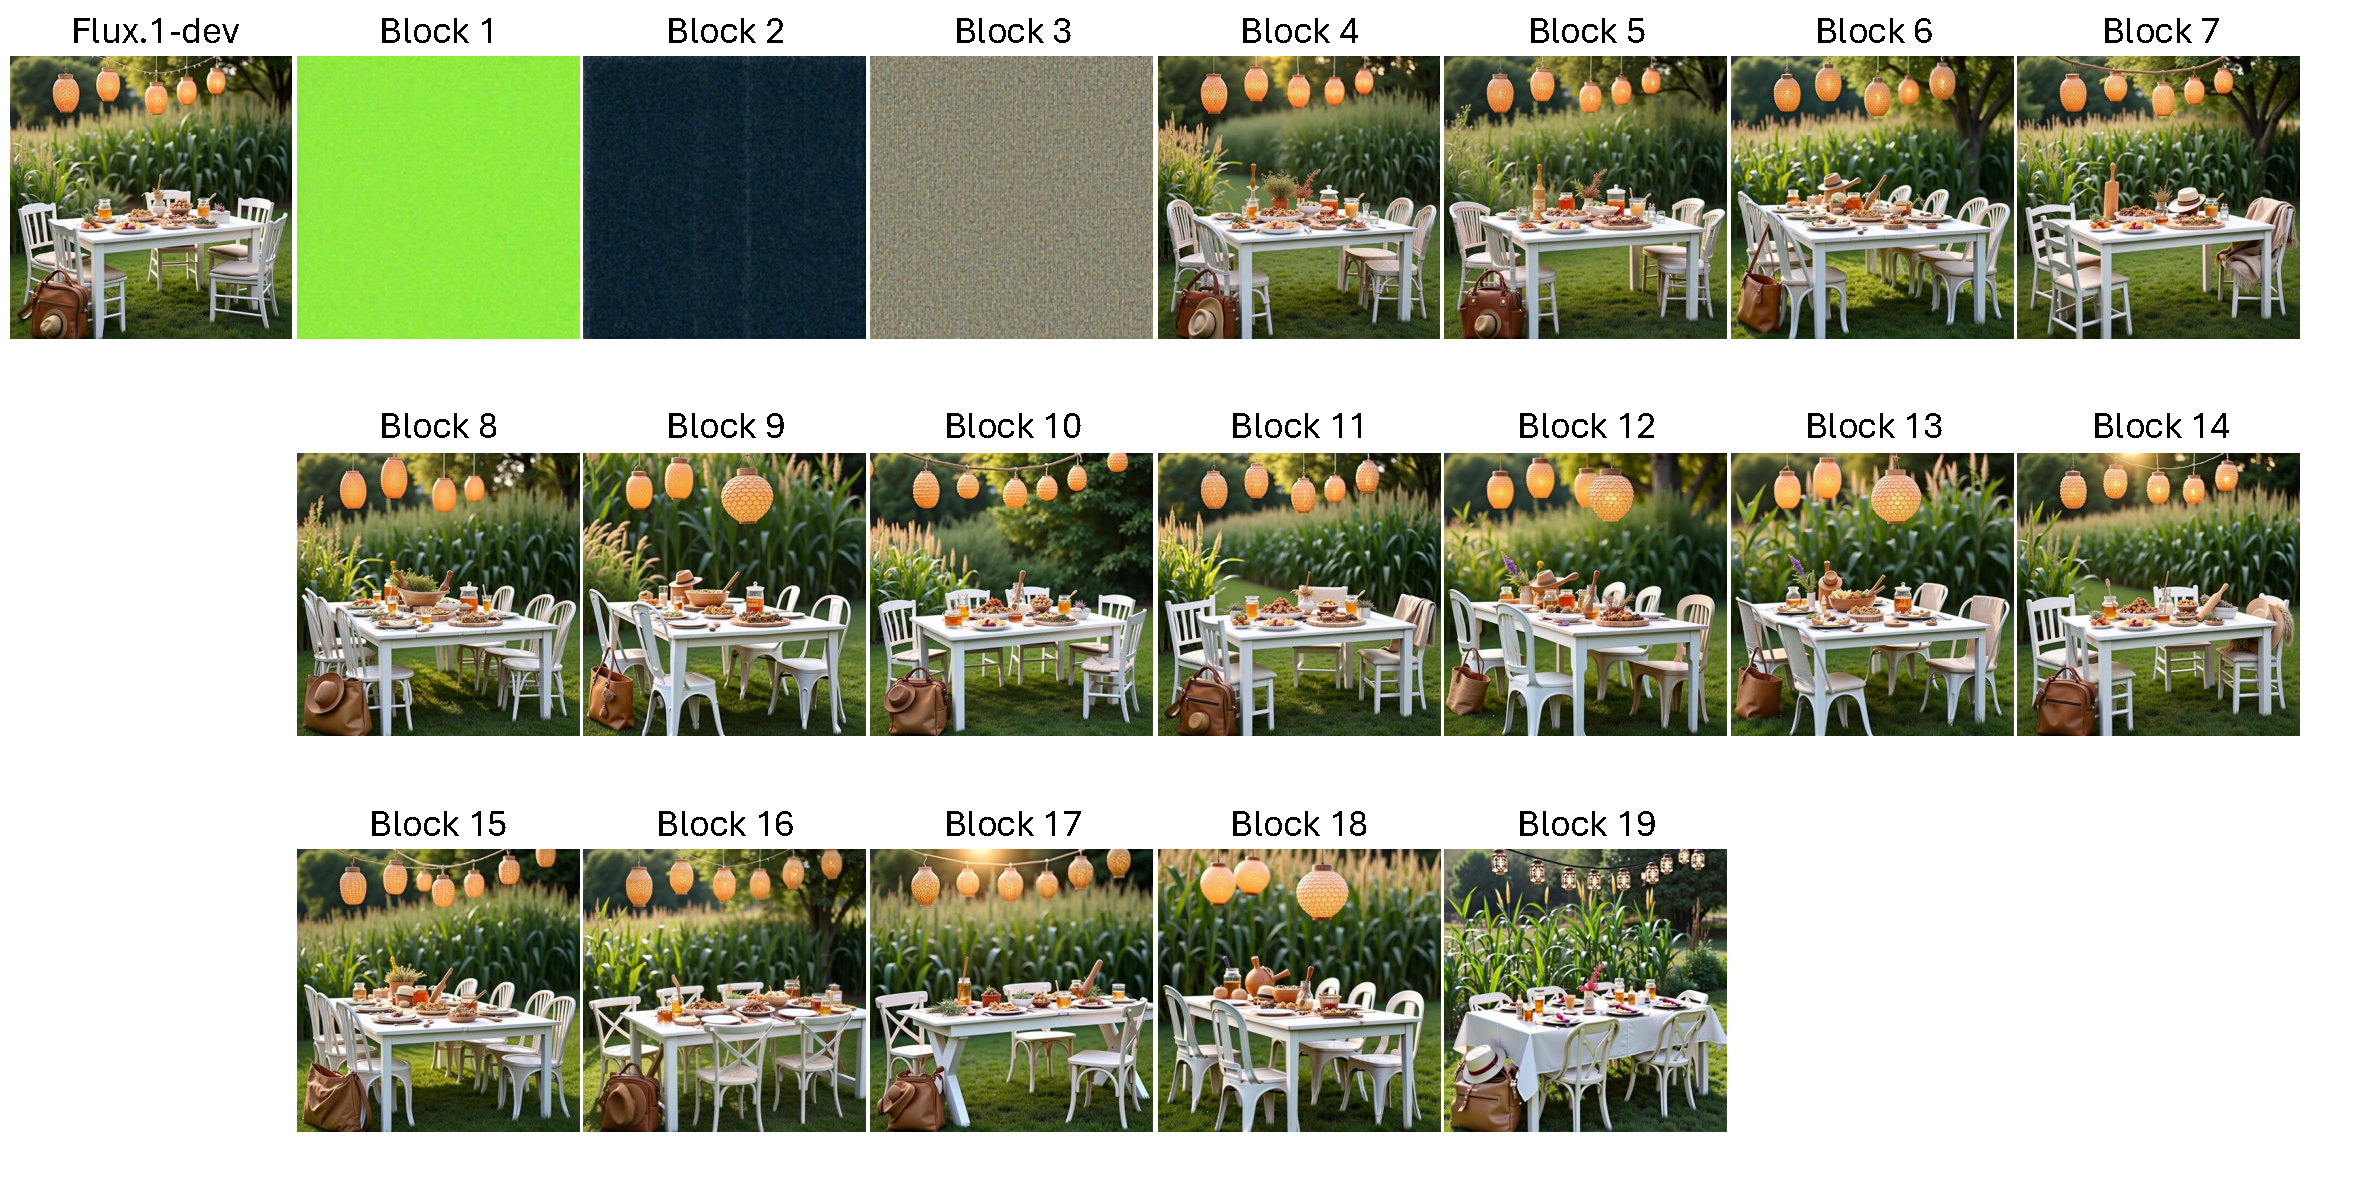
\includegraphics[width=\textwidth]{images/Experimente/Flux/Block_Analysis/BlockRemovalDouble.pdf}
\caption[Qualitative Double-Stream Block Importance Analysis of Flux.1-dev: Block Removal]{Qualitative comparison of the impact of complete removal of individual double-stream blocks in Flux.1-dev.}
	\label{fig:AppxBlockAnalysisRemovalDouble}
\end{figure}


\begin{figure}[H]
	\centering
	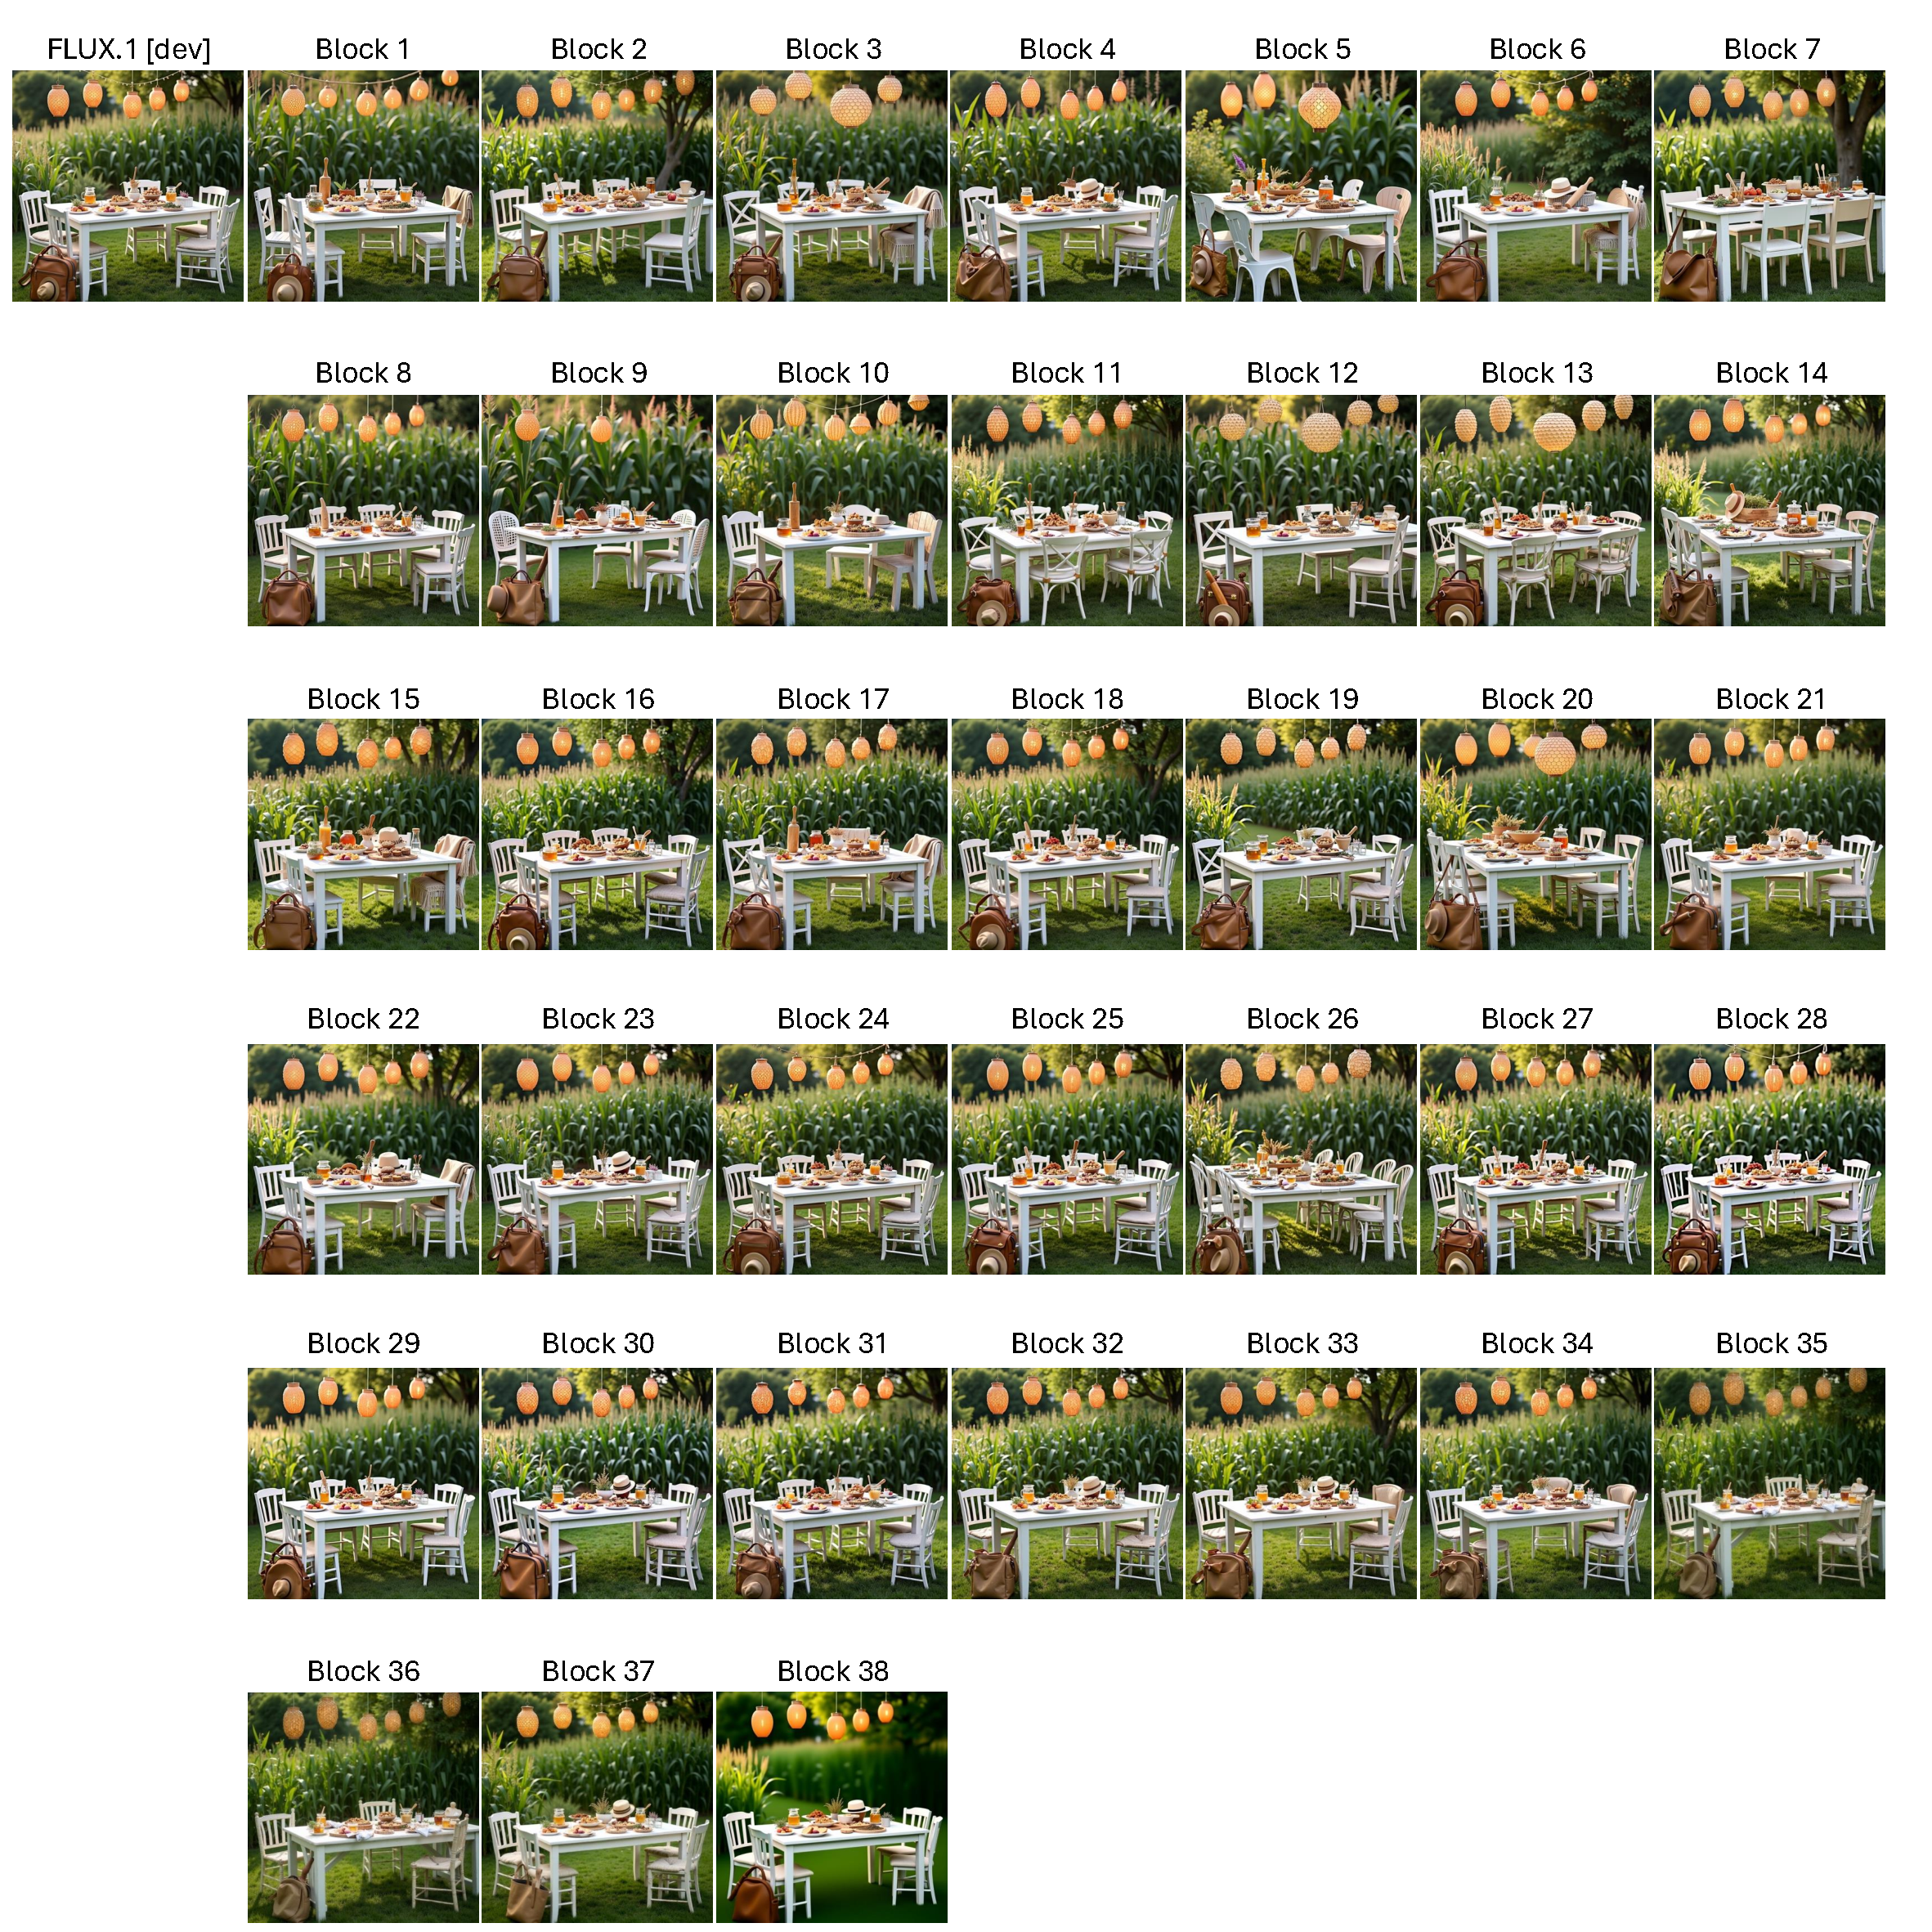
\includegraphics[width=\textwidth]{images/Experimente/Flux/Block_Analysis/BlockRemovalSingle.pdf}
\caption[Qualitative Single-Stream Block Importance Analysis of Flux.1-dev: Block Removal]{Qualitative comparison of the impact of complete removal of individual single-stream blocks in Flux.1-dev.}
	\label{fig:AppxBlockAnalysisRemovalSingle}
\end{figure}

\begin{figure}[H]
	\centering
	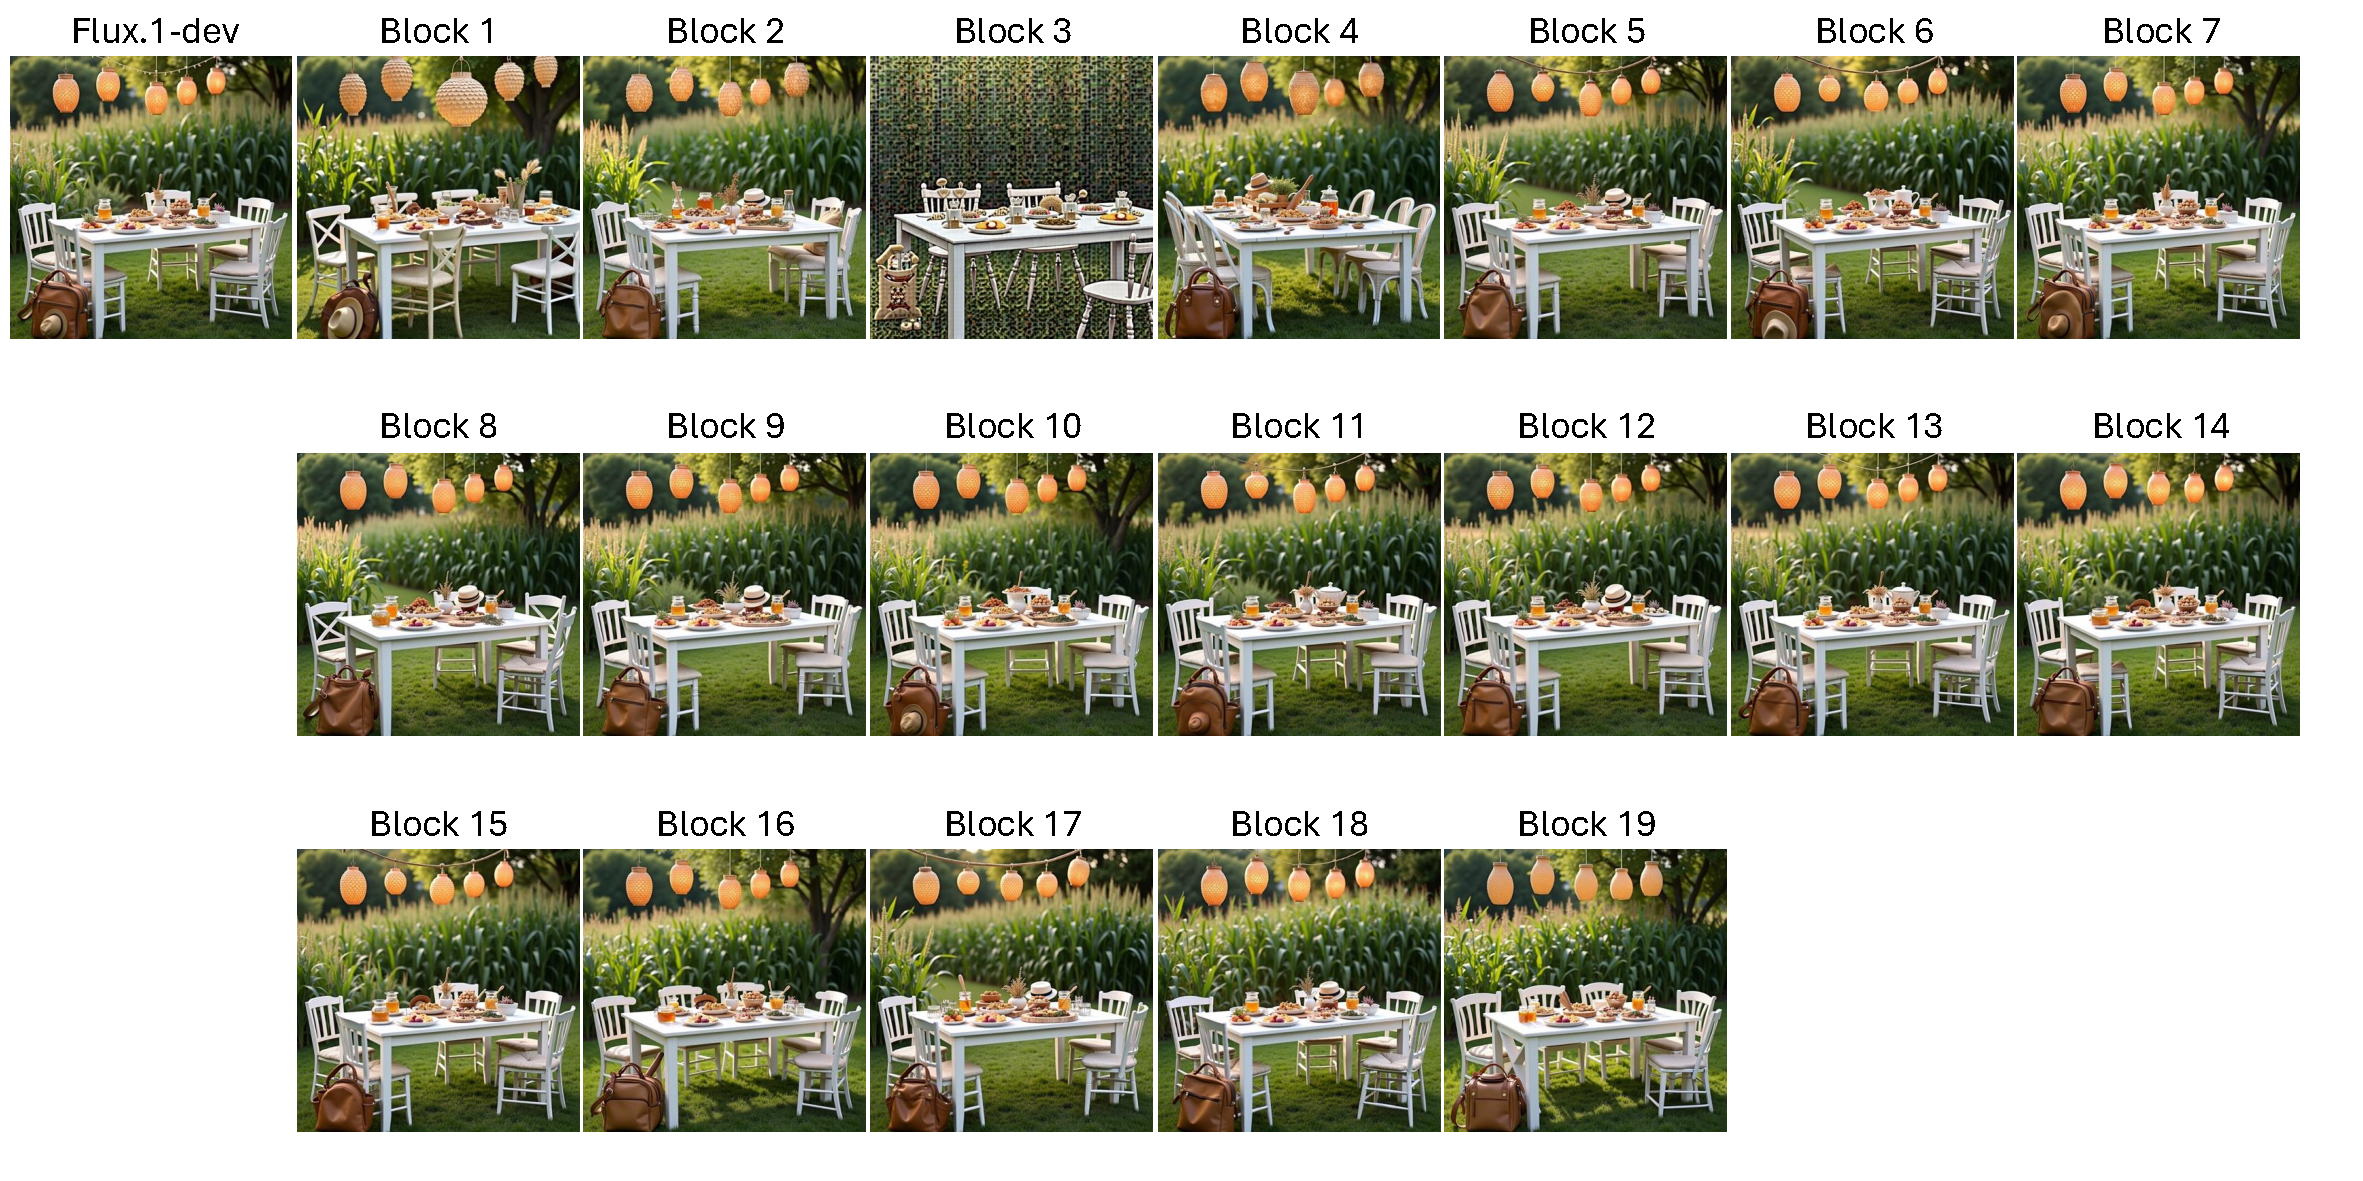
\includegraphics[width=\textwidth]{images/Experimente/Flux/Block_Analysis/BlockCompressionDouble.pdf}
\caption[Qualitative Double-Stream Block Importance Analysis of Flux.1-dev: Block Compression]{Qualitative comparison of the impact of 60\% compression of individual double-stream blocks in Flux.1-dev.}
	\label{fig:AppxBlockAnalysisCompressionDouble}
\end{figure}

\begin{figure}[H]
	\centering
	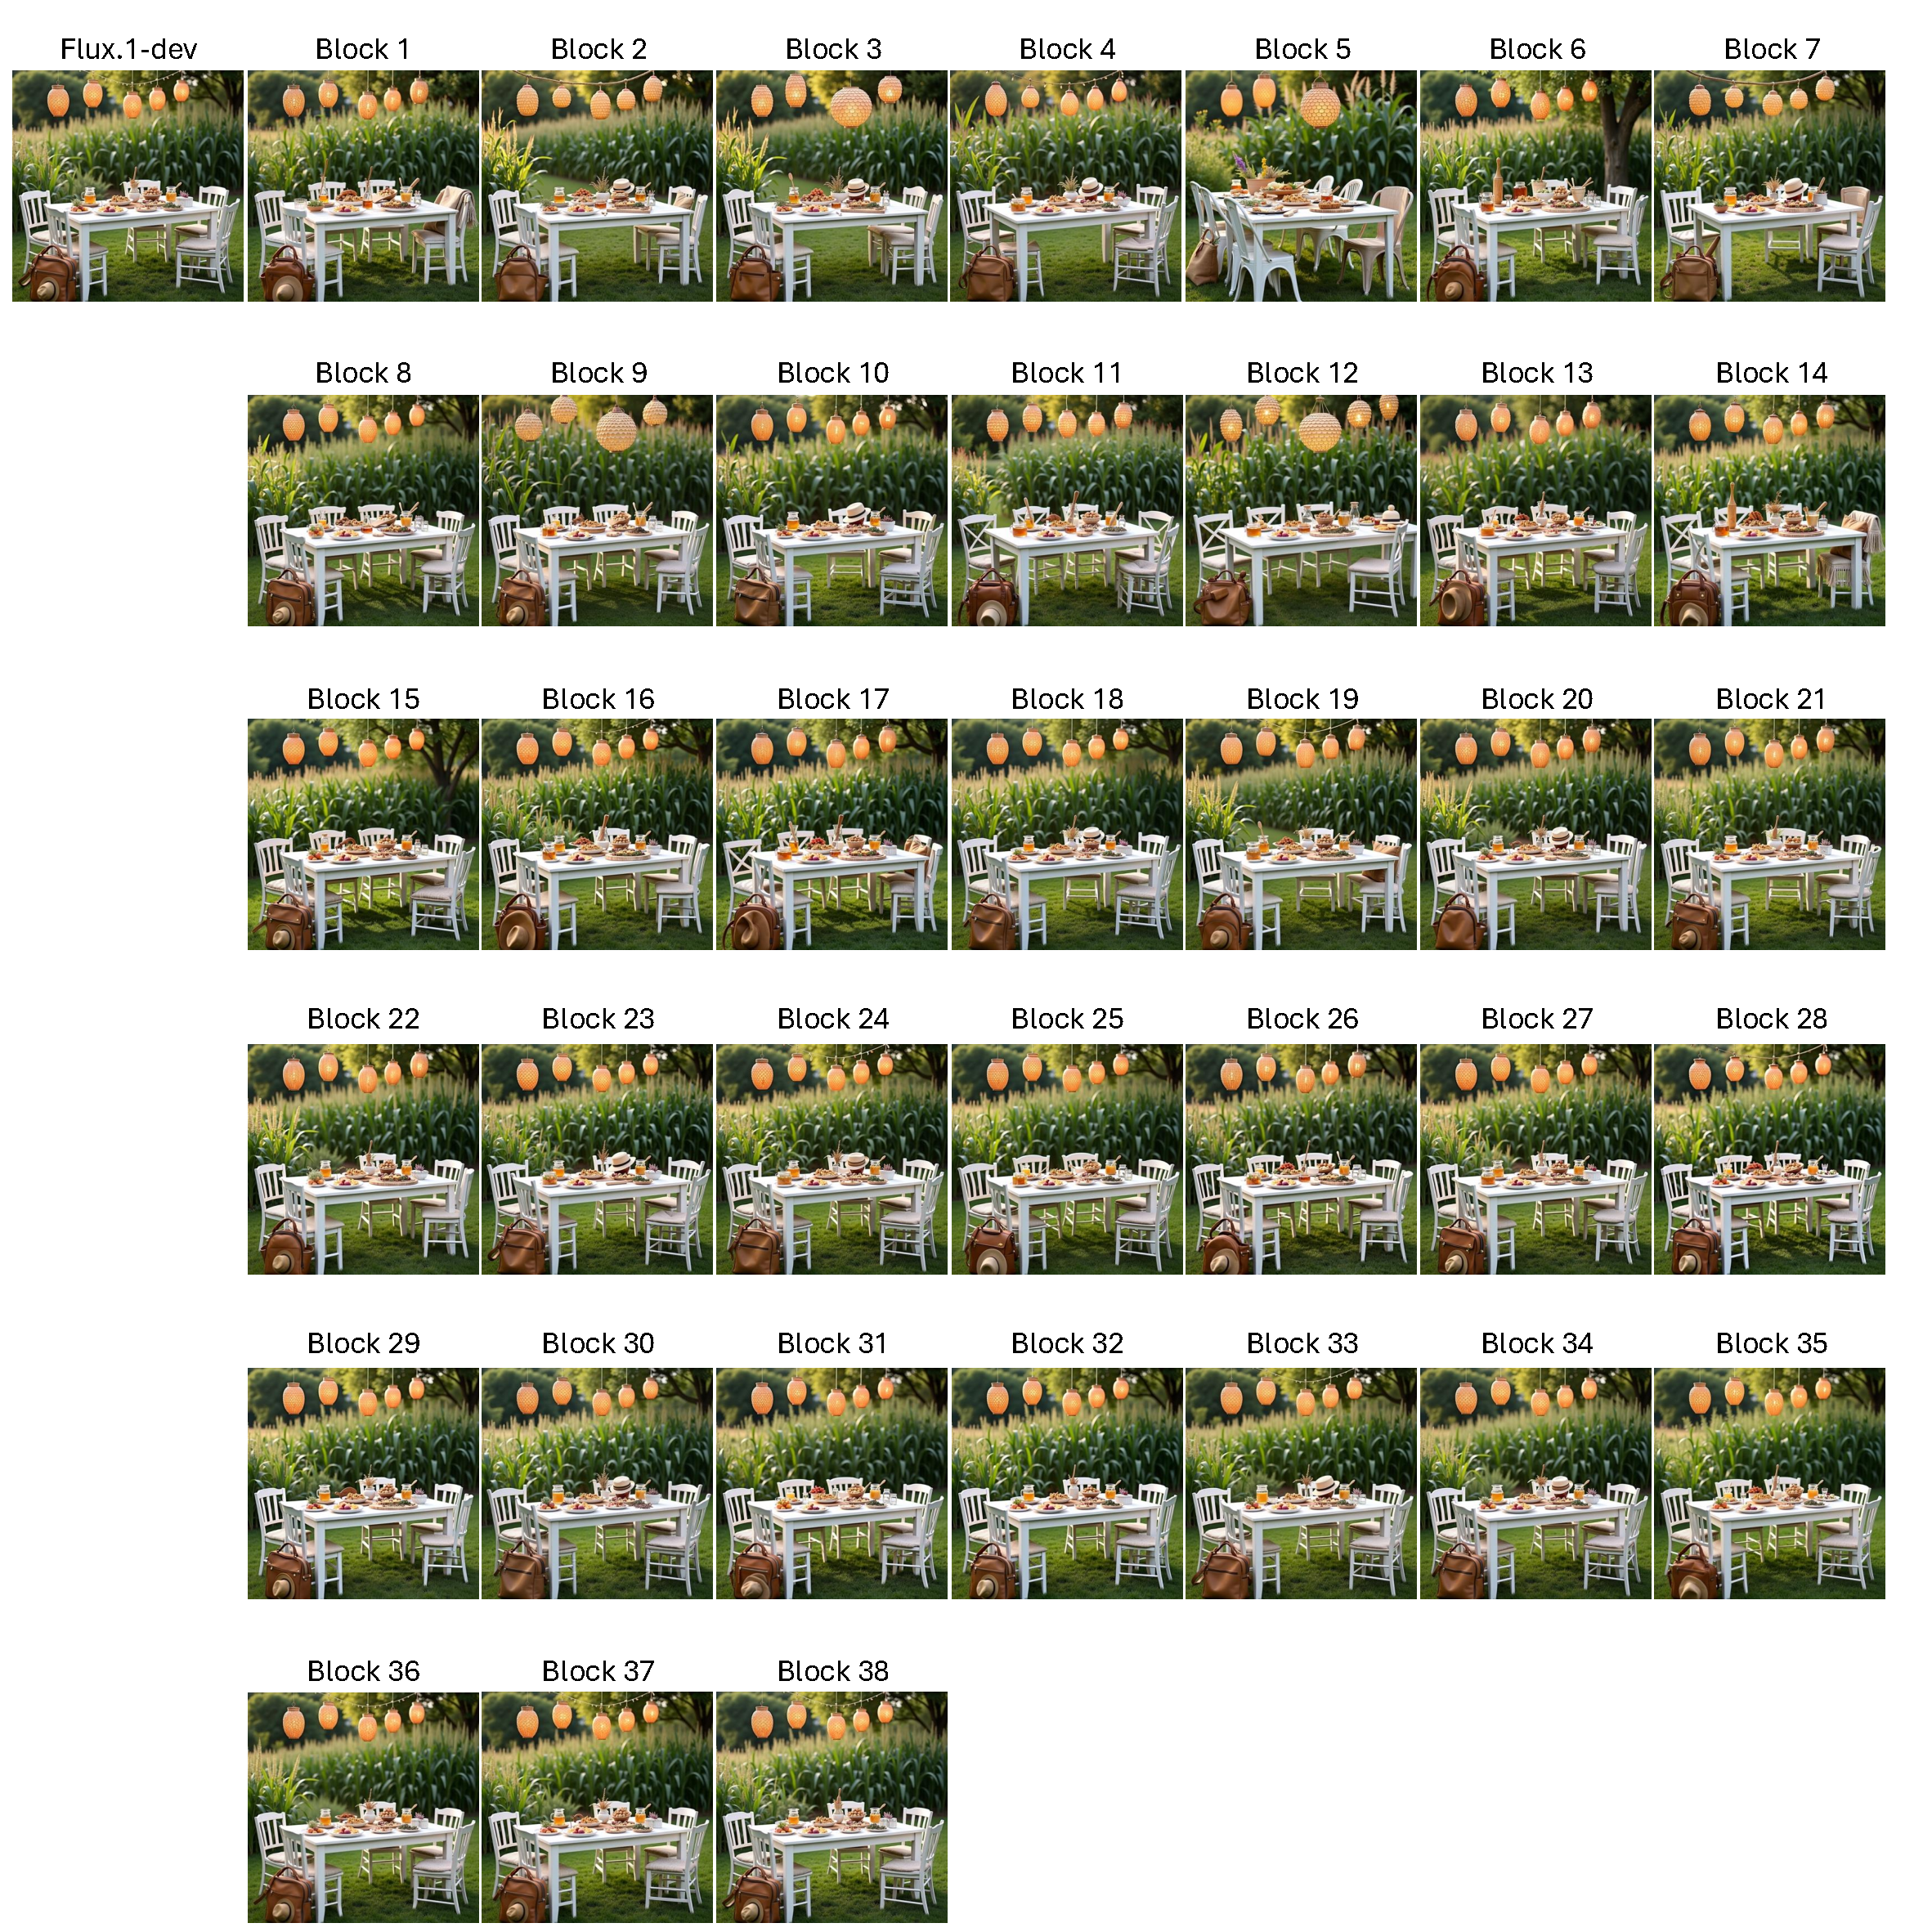
\includegraphics[width=\textwidth]{images/Experimente/Flux/Block_Analysis/BlockCompressionSingle.pdf}
\caption[Qualitative Single-Stream Block Importance Analysis of Flux.1-dev: Block Compression]{Qualitative comparison of the impact of 60\% compression of individual single-stream blocks in Flux.1-dev.}
	\label{fig:AppxBlockAnalysisCompressionSingle}
\end{figure}




\section{Training-Free Compression}
This section provides the technical settings for the training-free experiments (Sec. \ref{sec:trainingFreeCompression}) using complete block removal (\ref{tab:TrainingFreeMethodsRemoval}) and \gls{SVD}-based compression (Tab. \ref{tab:TrainingFreeMethodsSVD}). Furthermore, the example images for 90\% and 70\% models are provided (Fig. \ref{fig:Examples_TrainingFree90} - \ref{fig:Examples_TrainingFree70}).


	\begin{table}[H]
	\centering
	\caption[Training-Free Compression: \gls{SVD} Compression Details]{Details about importance-aware rank-adaptive progressive pruning schedule applied for \gls{SVD} based-compression in training-free setting.}
	\label{tab:TrainingFreeMethodsSVD}
	\begin{tabular}{@{}lccc@{}}
		\toprule
		\textbf{Model Size} & \textbf{Modified Blocks} & \textbf{Base Compression Ratio}  & \textbf{Slope $x$}  \\ \midrule
		90\% & 30 & 25\% & 0.0083 \\
		80\% & 30 & 50\% & 0.0166\\
		70\% & 30 & 75\% & 0.0249\\
		\bottomrule
	\end{tabular}
\end{table}

	\begin{table}[H]
	\centering
	\caption[Training-Free Compression: Complete Block Removal Details]{Details about complete block removal scheme in training-free setting.}
	\label{tab:TrainingFreeMethodsRemoval}
	\begin{tabular}{@{}lccc@{}}
		\toprule
		\textbf{Model Size} & \textbf{No. Removed Blocks} & \textbf{Removed Double Blocks}   \\ \midrule
		90\% & 3 & 13,16,5\\
		80\% & 7 & 13, 16, 5, 3, 17, 8, 15\\
		70\% & 10 & 13, 16, 5, 3, 17, 8, 15, 6,14, 18\\
		\bottomrule
	\end{tabular}
\end{table}


	\begin{figure}[H]
	\centering
	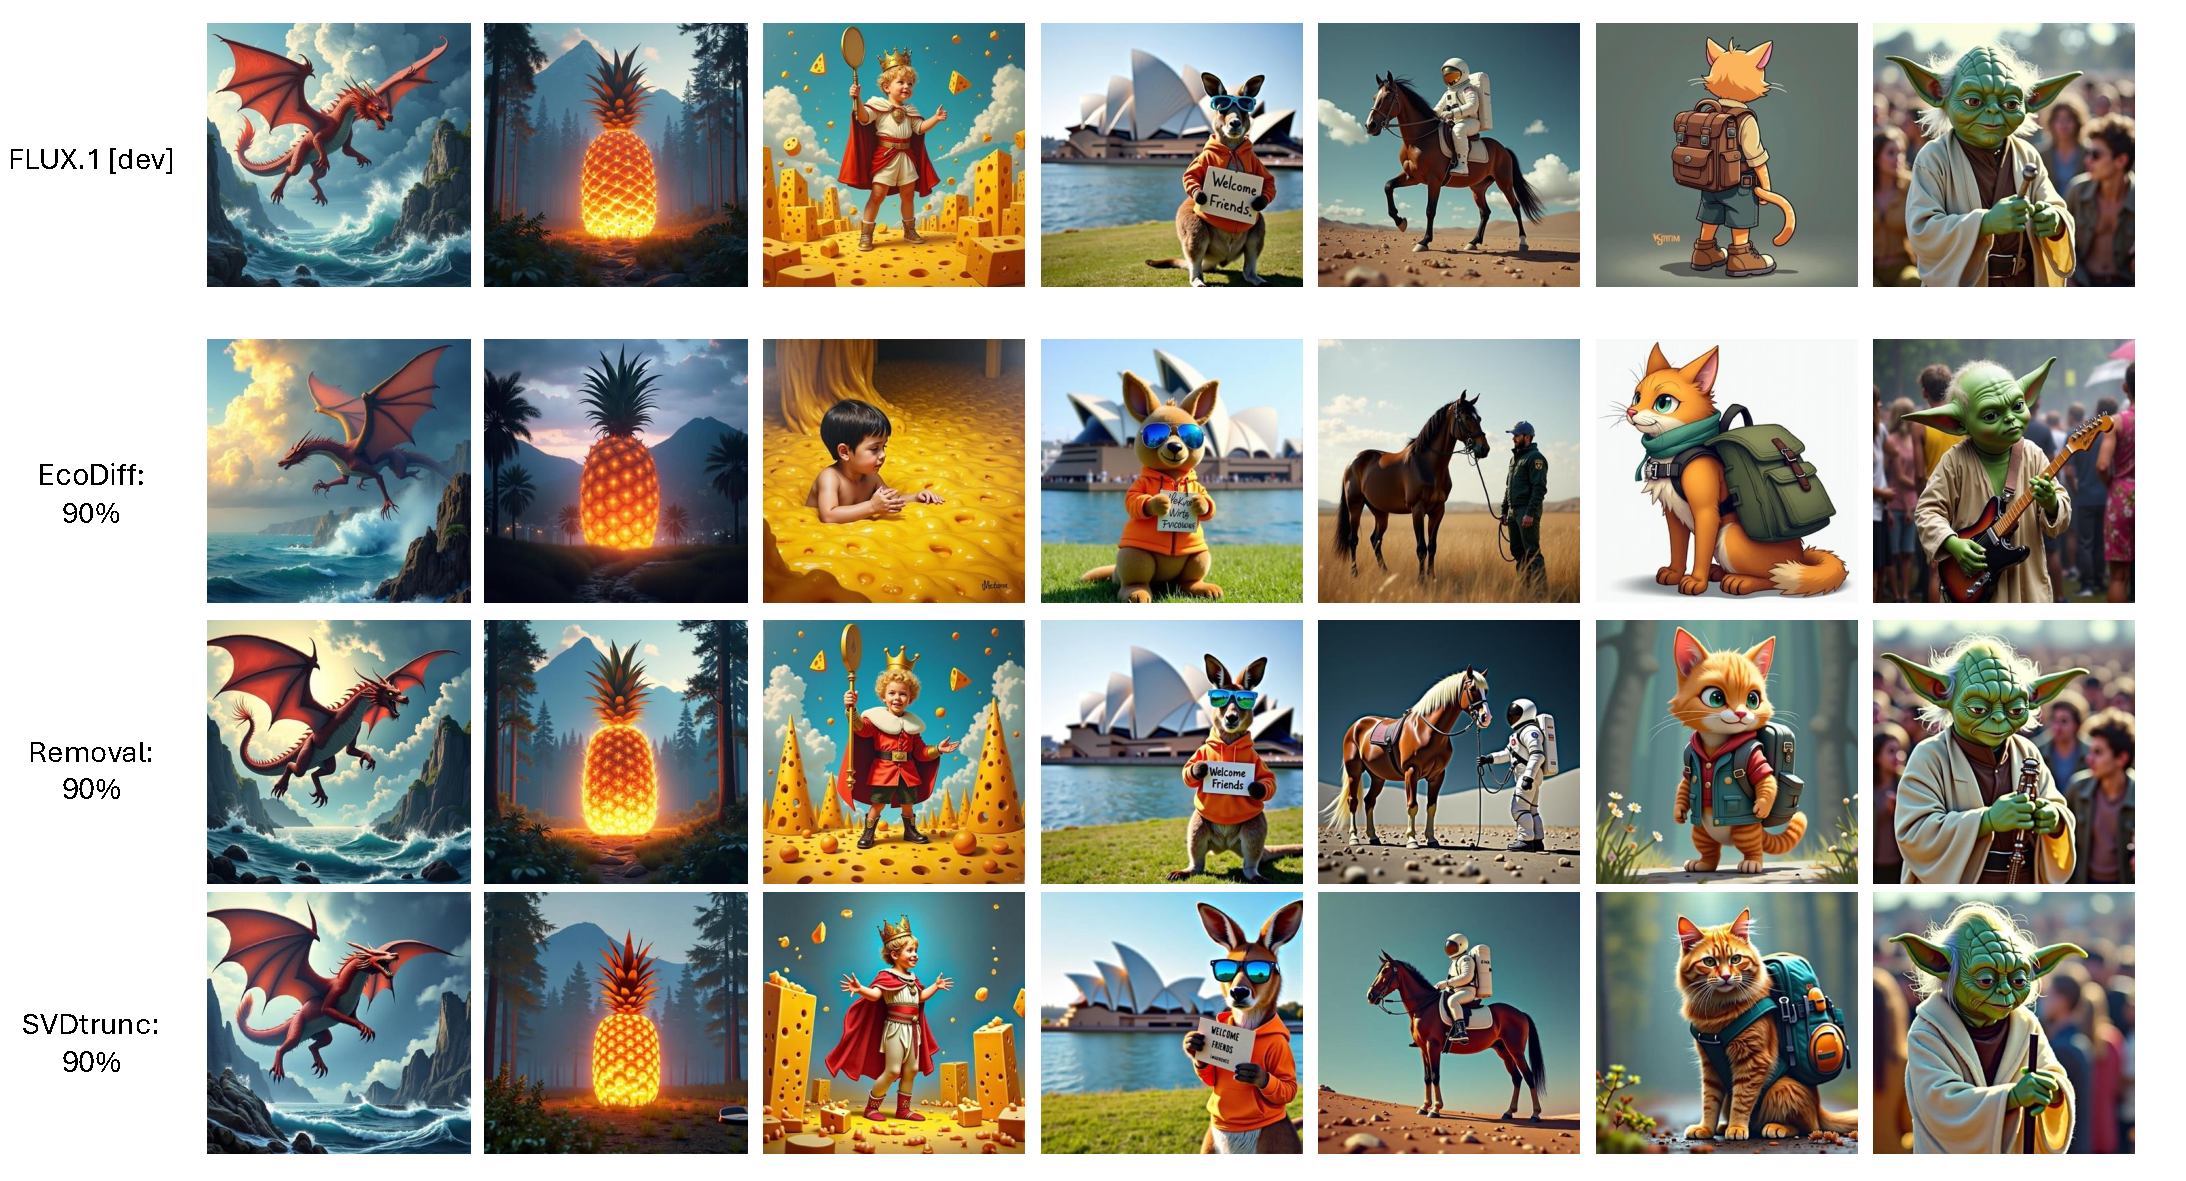
\includegraphics[width=\textwidth]{images/Experimente/Flux/TrainingFree_paper/TrainingFreeAppendix_model90.pdf}
	\caption[Qualitative Examples: Training-Free Model Compression (90\% Pruning)]{Qualitative comparison of example images generated by models pruned to 90\% using EcoDiff, complete block removal, and truncated \gls{SVD} compression without fine-tuning.}
	\label{fig:Examples_TrainingFree90}
\end{figure}

	\begin{figure}[H]
	\centering
	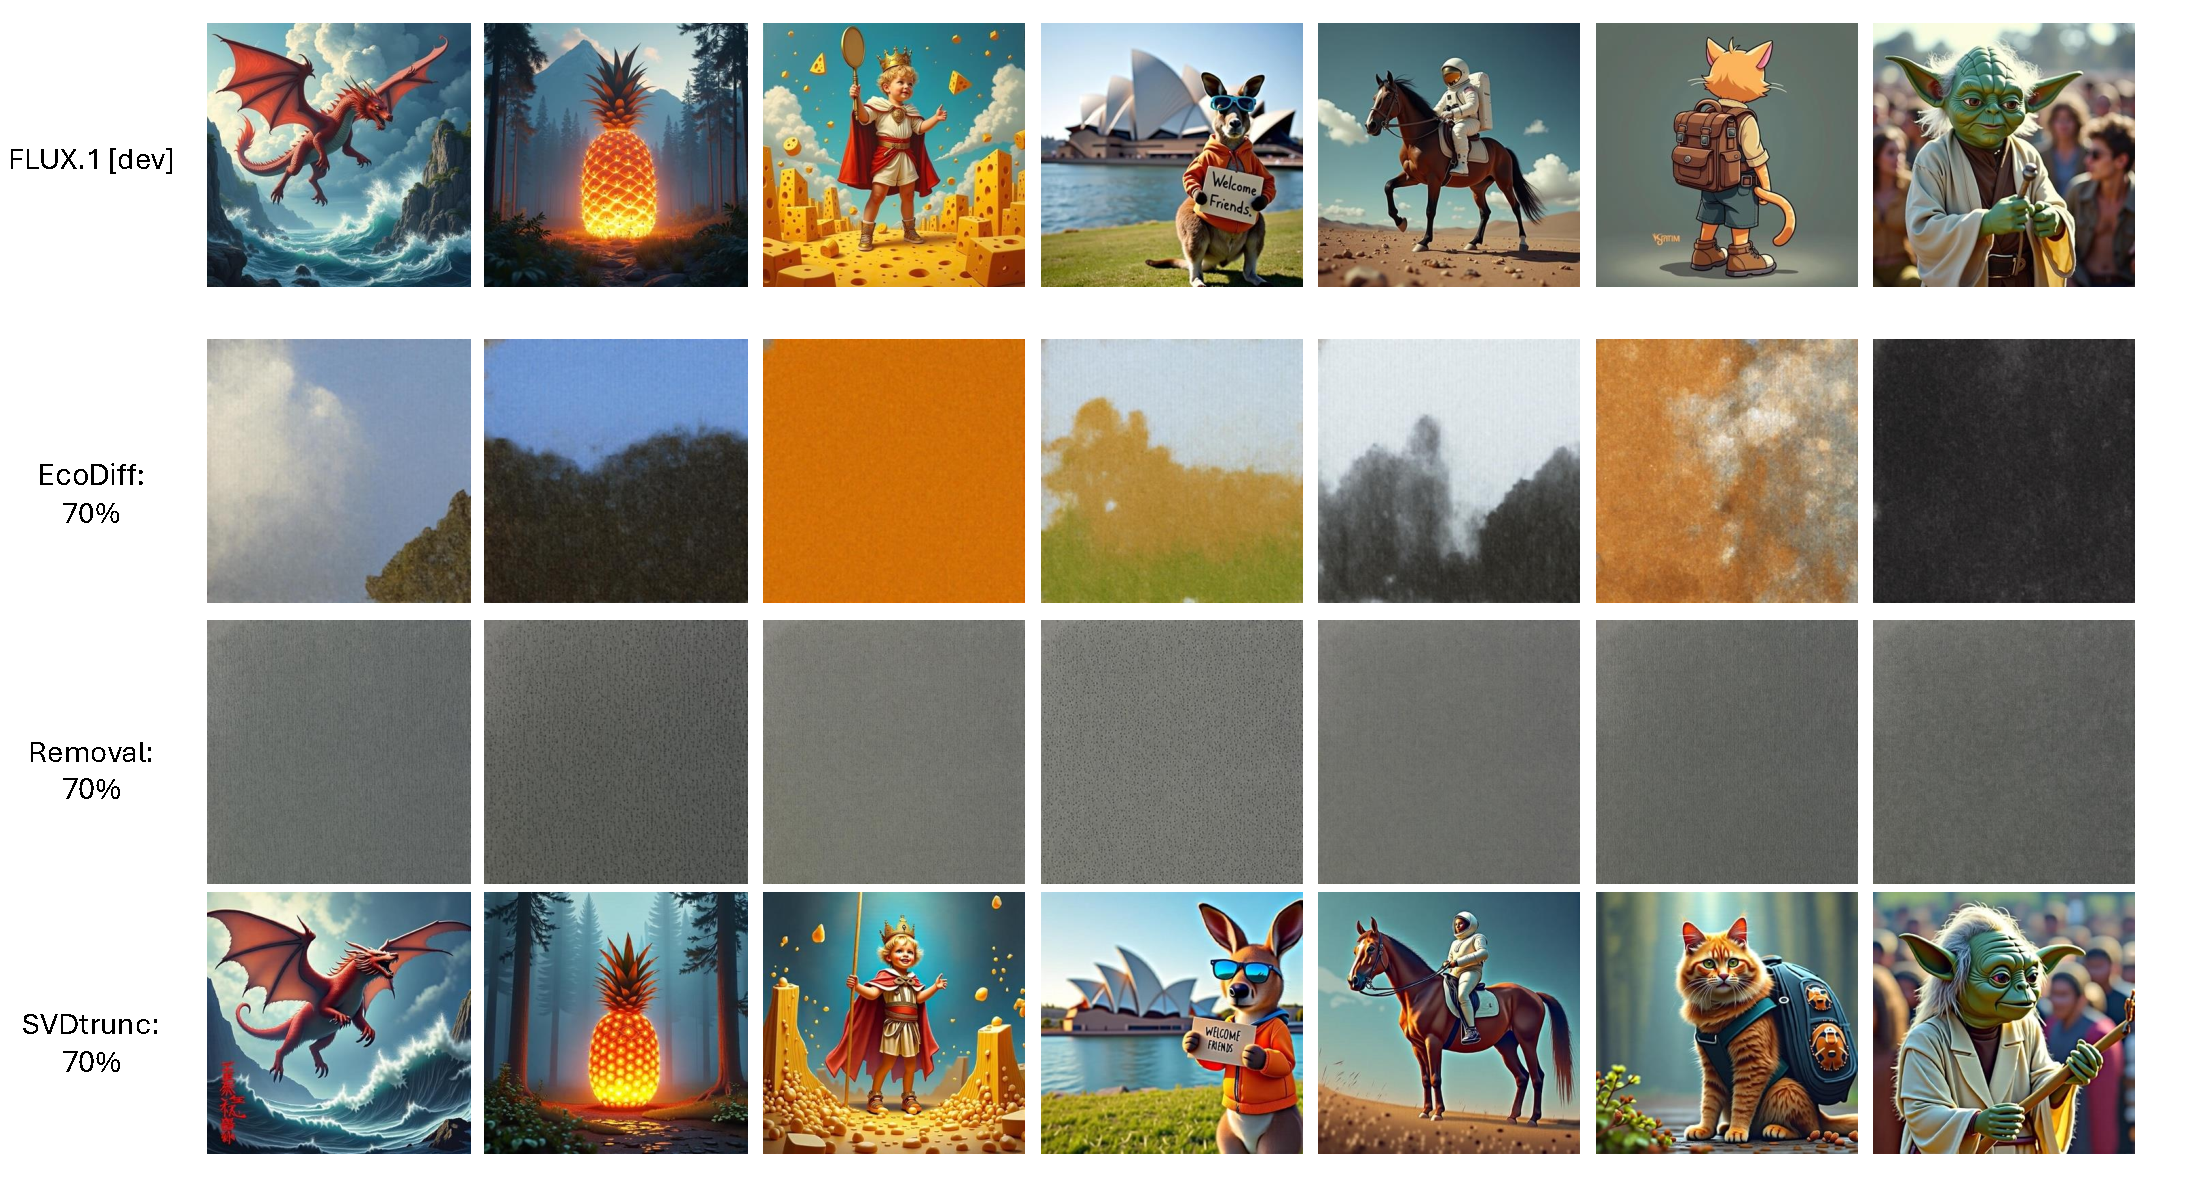
\includegraphics[width=\textwidth]{images/Experimente/Flux/TrainingFree_paper/TrainingFreeAppendix_model70.pdf}
	\caption[Qualitative Examples: Training-Free Model Compression (70\% Pruning)]{Qualitative comparison of example images generated by models pruned to 70\% using EcoDiff, complete block removal, and truncated \gls{SVD} compression without fine-tuning.}
	\label{fig:Examples_TrainingFree70}
\end{figure}

\section{Importance-Aware Low-Rank Model Compression - Preliminary Experiments}

\subsection{Block Selection}
\label{sec:FluxBlockImportanceAnalysisAppendix}
Tab. \ref{tab:Random_vs_metric_Selection} summarizes the experimental settings for the block selection analysis presented in Section \ref{sec:FluxBlockImportanceAnalysis}. Furthermore, this subsection provides qualitative example images (Figs. \ref{fig:FluxBlockSelection_68}--\ref{fig:FluxBlockSelection_43}) generated by Flux.1-dev models at various compression stages. These results were obtained utilizing random, uniform, and importance-aware block selection strategies.


\begin{table}[h]
	\centering
	\caption[Block Selection: Compression Details]{Overview of compression and fine-tuning details for both experiments, random and metric-based block selection.}
	\label{tab:Random_vs_metric_Selection}
	\begin{tabular}{c c c c c}
		\toprule
		\textbf{Iteration} & \textbf{Model Size (\%)} & \textbf{Blocks} \footnotemark & \textbf{Training Steps} \\
		& & & \textbf{per Iteration} \\
		\midrule
		1 & 68\% & 48   & 40k \\ % Beispielwerte
		2 & 57\% & 30  & 20k \\
		3 & 49\% & 30  & 20k \\
		4 & 43\% & 30 & 20k \\
		\bottomrule
	\end{tabular}
\end{table}
\footnotetext{The number of blocks are only relevant for the random and importance-based block selection experiments. For the uniform experiments all blocks were modified per iteration.}



\begin{figure}[H]
	\centering
	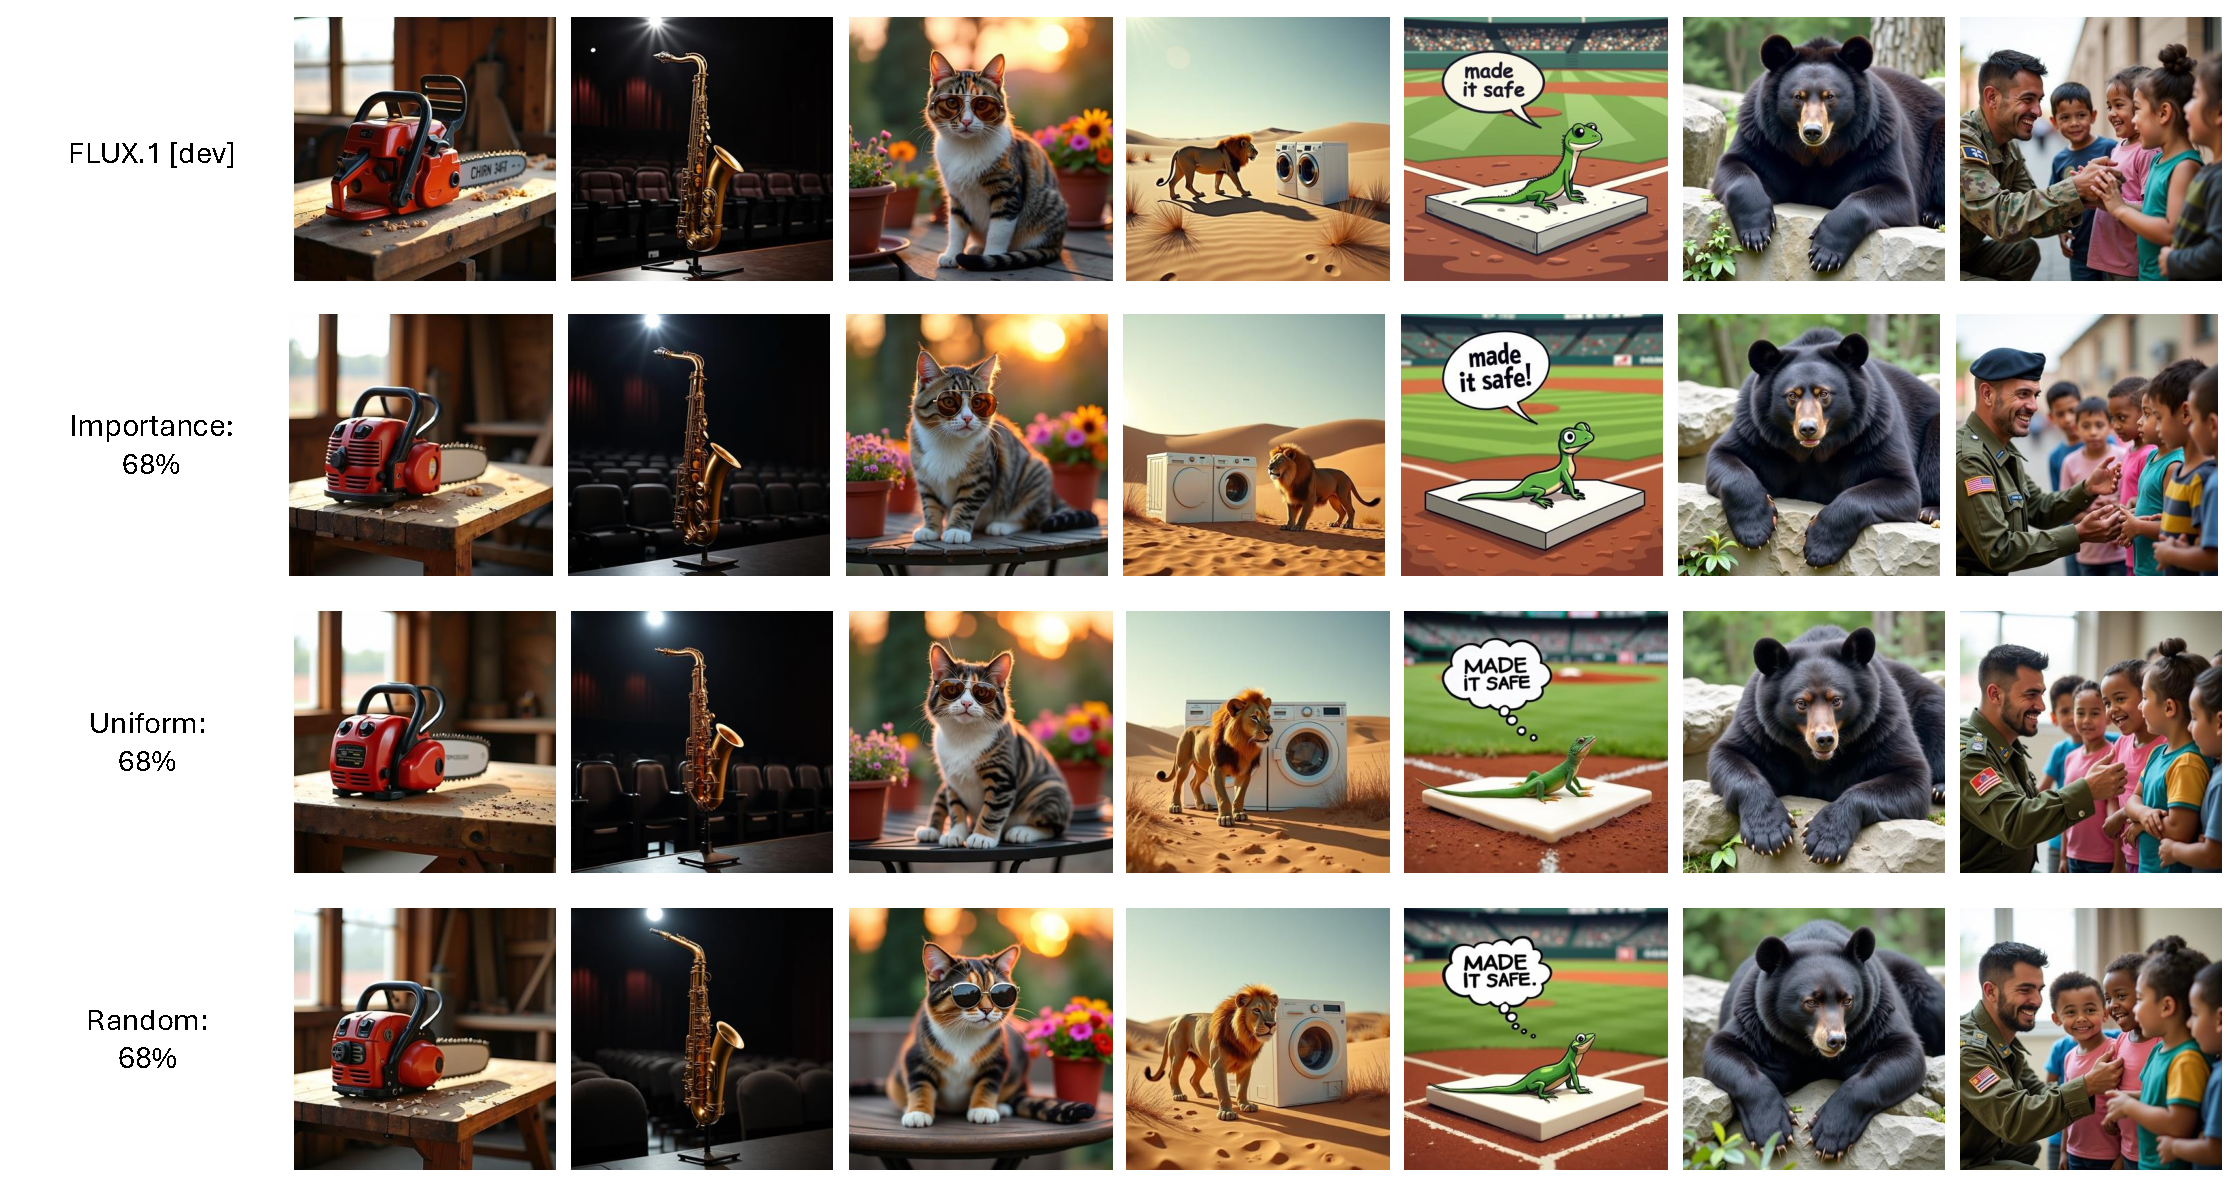
\includegraphics[width=\textwidth]{images/Experimente/Flux/BlockSelection/Random_vs_Importance_Block_Selection_Appendix_model_68.pdf}
	\caption[Qualitative Examples: Importance, Uniform, and Random Block Selection (68\% Pruning)]{Qualitative comparison of example images generated by models pruned to 68\% obtained by random, uniform, and importance-based block selection.}
	\label{fig:FluxBlockSelection_68}
\end{figure}
\begin{figure}[H]
	\centering
	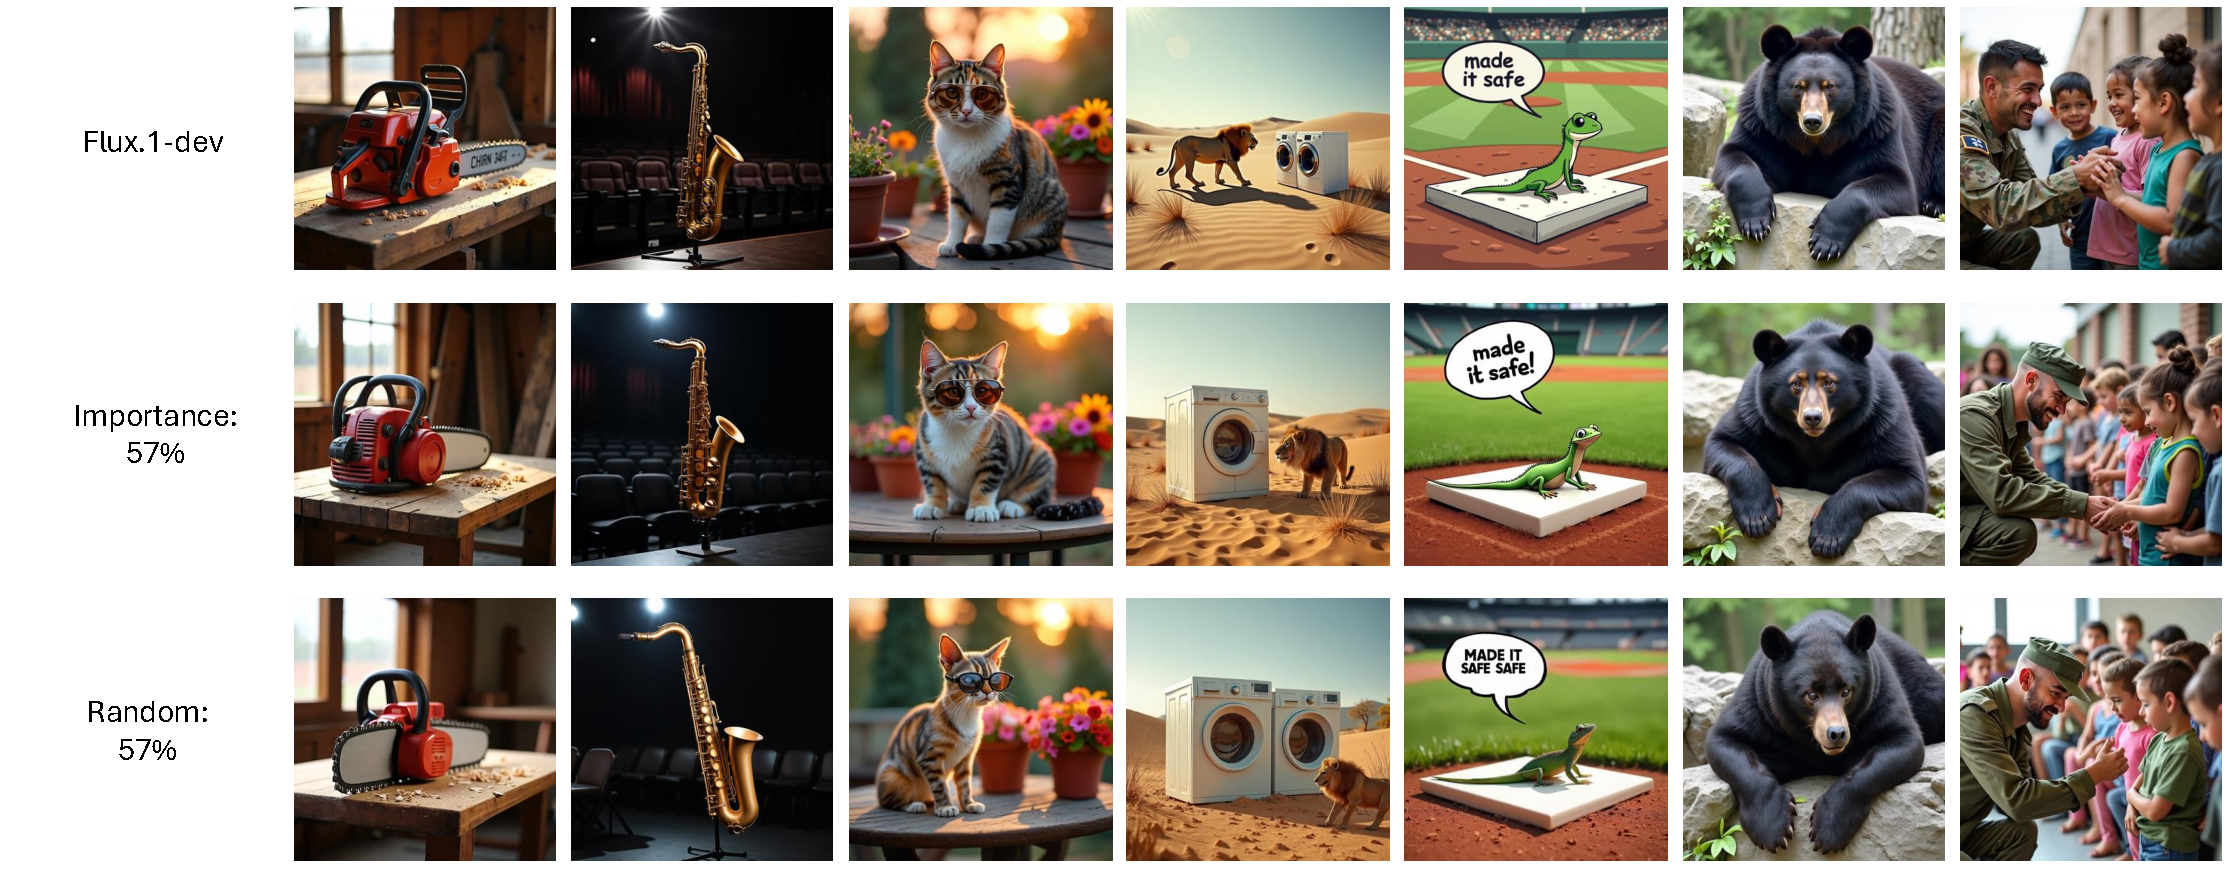
\includegraphics[width=\textwidth]{images/Experimente/Flux/BlockSelection/Random_vs_Importance_Block_Selection_Appendix_model_57.pdf}
\caption[Qualitative Examples: Importance, Uniform, and Random Block Selection (57\% Pruning)]{Qualitative comparison of example images generated by models pruned to 57\% obtained by random, uniform, and importance-based block selection.}
\label{fig:FluxBlockSelection_57}
\end{figure}
\begin{figure}[H]
	\centering
	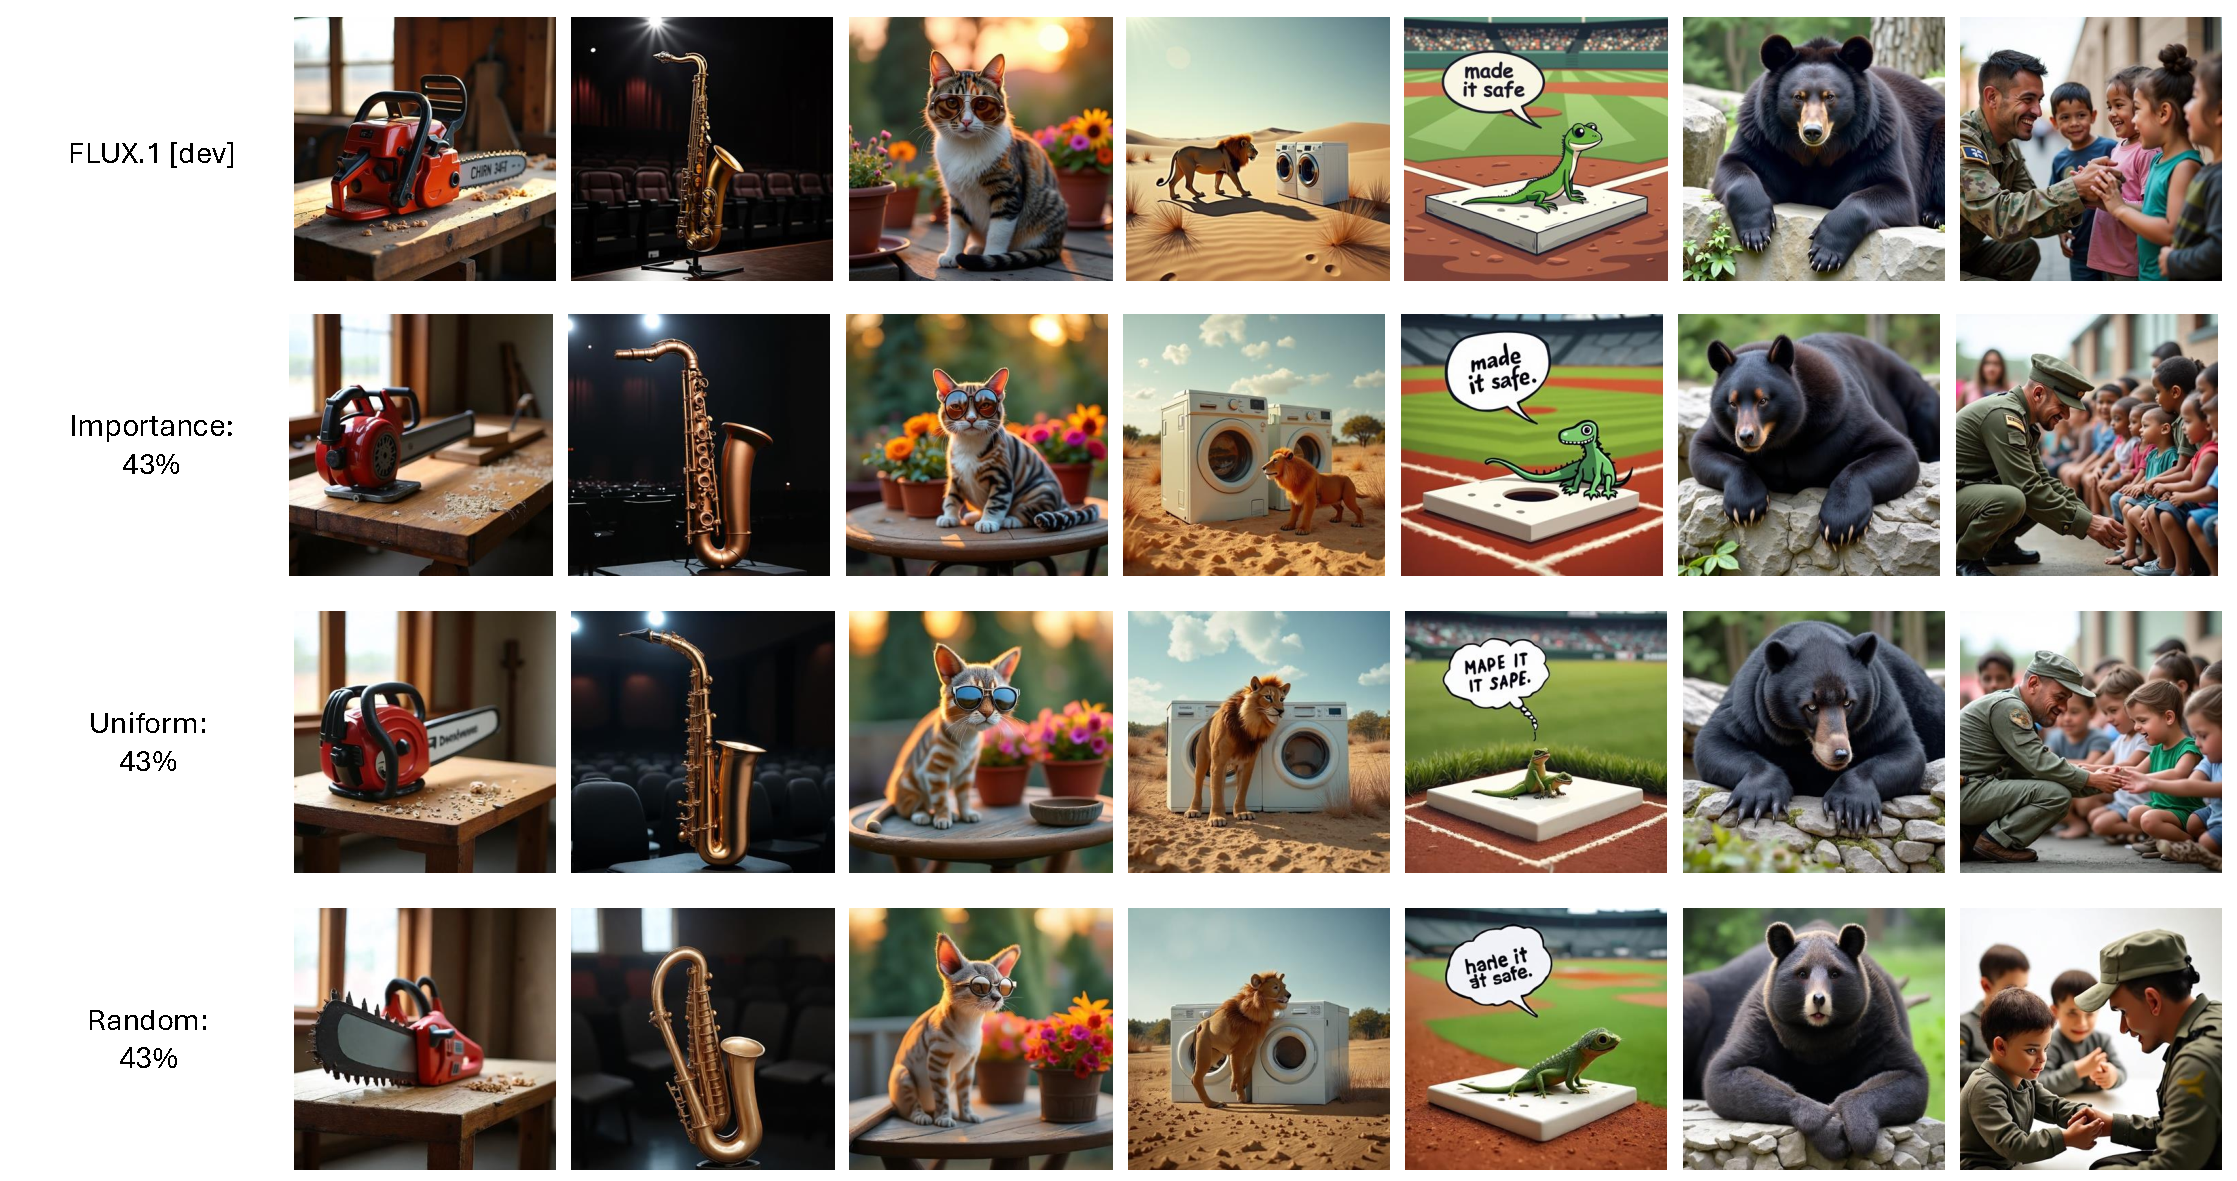
\includegraphics[width=\textwidth]{images/Experimente/Flux/BlockSelection/Random_vs_Importance_Block_Selection_Appendix_model_43.pdf}
\caption[Qualitative Examples: Importance, Uniform, and Random Block Selection (43\% Pruning)]{Qualitative comparison of example images generated by models pruned to 43\% obtained by random, uniform, and importance-based block selection.}
\label{fig:FluxBlockSelection_43}
\end{figure}

\subsection{Sensitivity Analysis: The Role of Parameter Removal Distribution}
Tab. \ref{tab:compression_iterations} summarizes the experimental settings for the importance-aware rank-adaptive progressive pruning schedule. These configurations are used to investigate how to optimally distribute the removed parameters across a varying number of Transformer blocks, as detailed in Section \ref{sec:FluxParameterRemovalDistribution}.





\begin{table}[H]
	\centering
\caption[Parameter Removal Distribution: Compression Details]{Overview of the experimental settings for the importance-aware rank-adaptive progressive pruning schedule, detailing how the removed parameters are distributed across varying numbers of blocks. For readability, we provide the slope $x$ scaled by 1000.}
	\label{tab:compression_iterations}
	\begin{tabular}{ccccc}
		\toprule
		\textbf{Iteration} &\textbf{Model Size} & \textbf{Number of} & \textbf{Base Compression} & \textbf{Slope} $x$\\
		&&\textbf{Modified Blocks}&\textbf{Ratio}& \\
		\midrule
		\multicolumn{5}{c}{Flux.1.dev\cite{Flux}}\\
		\midrule
		\multirow{3}{*}{1} 
		& \multirow{3}{*}{90\%}  
		& 20 & 0.3 & 12.8 \\
		&  &   30 & 0.25 & 8.3 \\
		&  & 40  & 0.2 & 4.3 \\
		\midrule
		\multirow{3}{*}{2} 
		& \multirow{3}{*}{80\%} 
		 & 20 & 0.3 & 8.2 \\
		&  &   30 & 0.25 & 5.9 \\
		&  & 40  & 0.2 & 3.4  \\
		\midrule
		\multirow{3}{*}{3} 
		& \multirow{3}{*}{70\%}  
		& 20 & 0.4 & 11.7  \\
		&  &   30 & 0.3  & 6.7 \\
		&  & 40  & 0.25 & 4.9  \\
		\midrule
		\multirow{3}{*}{4} 
		& \multirow{3}{*}{60\%}  & 20 & 0.5 & 4.0  \\
		&  &   30 & 0.35  & 6.8 \\
		&  & 40  & 0.25 & 3.0 \\
		\midrule
		\multirow{3}{*}{5} 
		& \multirow{3}{*}{50\%}  & 20 & 0.6 & 18.0  \\
		&  &   30 & 0.4 & 4.9 \\
		&  & 40  & 0.35 & 0.71  \\
		
			\midrule
		\multirow{3}{*}{6} 
		& \multirow{3}{*}{40\%}  
		& 20 & 0.6 &  36.7 \\
		&  &   30 & 0.4 & 2.7 \\
		&  & 40  & 0.4& 5.6  \\
		
		\bottomrule
	\end{tabular}
\end{table}


\section{Importance-Aware Rank-Adaptive Low-Rank Model Compression}
\label{sec:Appendix_SVDtrunc}
This section provides details of the best models obtained via \gls{SVD}trunc of Flux.1-dev. Tab. \ref{tab:sup_training} depicts the settings for the importance-aware rank-adaptive pruning framework. Tab. \ref{tab:sup_hps} - \ref{tab:sup_dpg} provides the detailed values obtained for the HPSv2, GenEval and DPG benchmarks for these models. 

In addition, further example images for \gls{SVD}trunc \ref{fig:SVDtrunc_Appx} as well as of the observed domain shift (Fig. \ref{fig:SVDtruncFlux_ShiftAppx}) and memorization loss (Fig. \ref{fig:SVDtrunc_Memorization_Loss_Appx}) are presented.


	\begin{figure}[H]
	\centering
	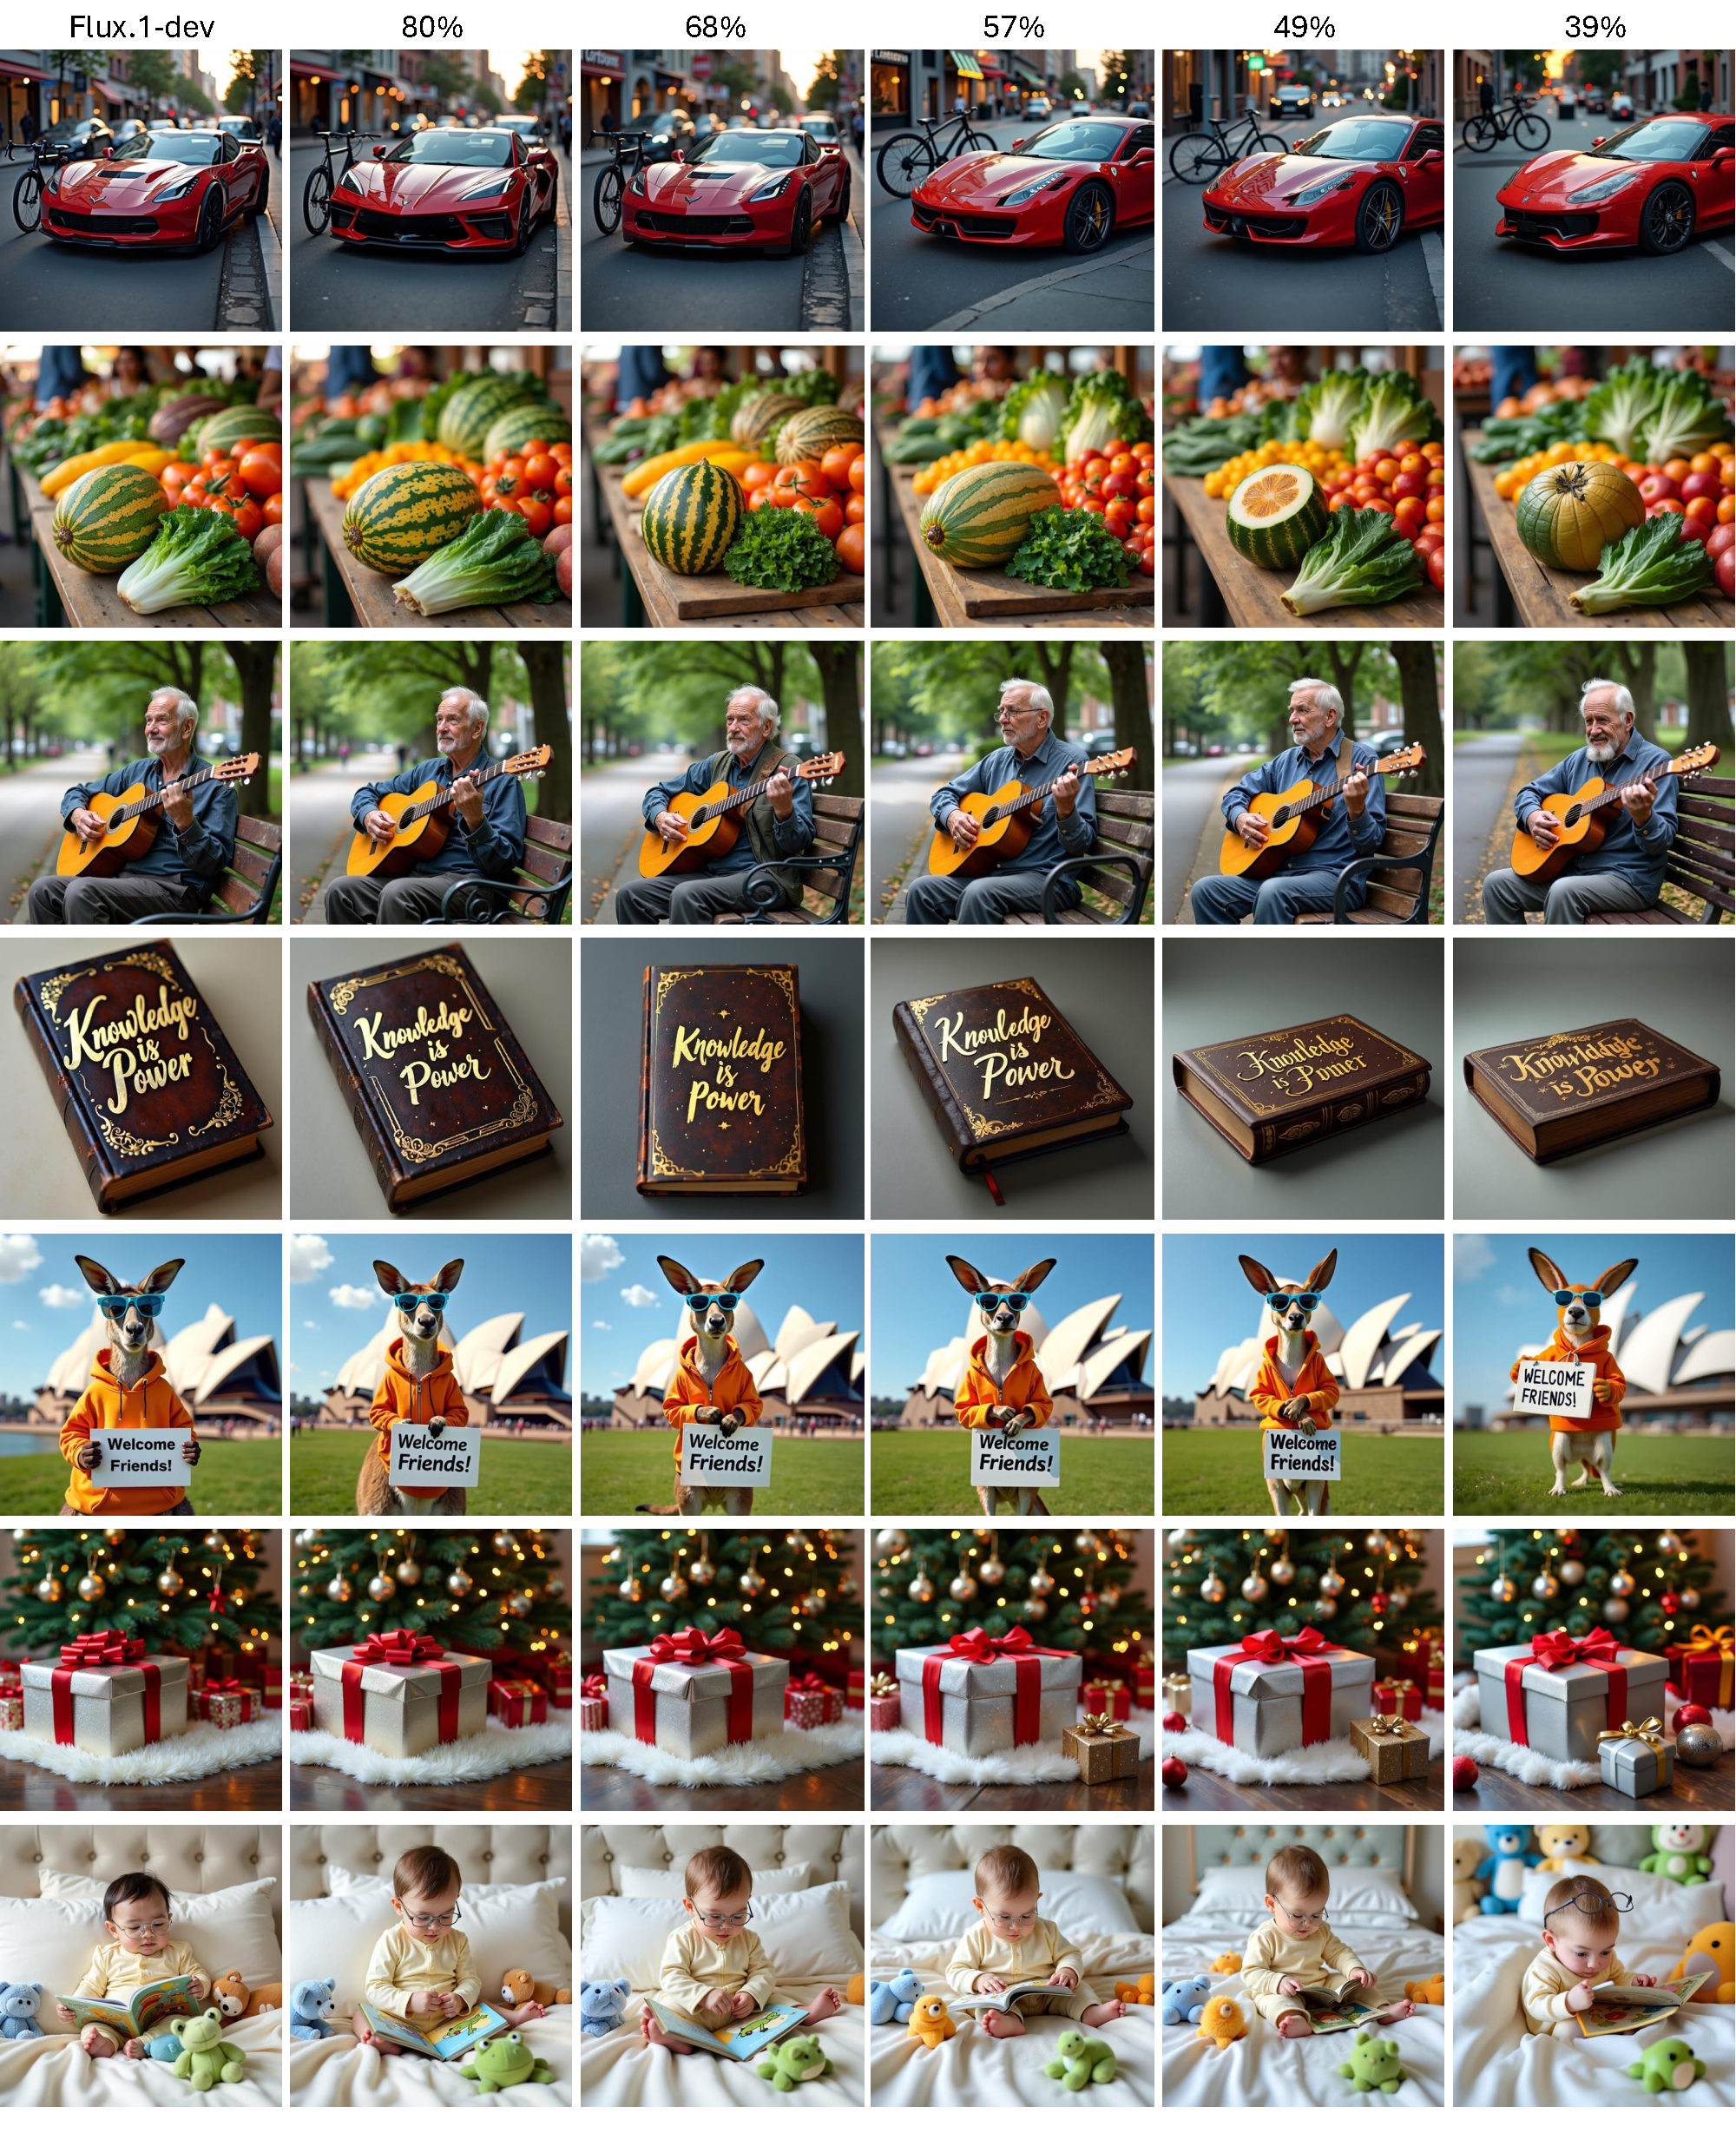
\includegraphics[width=\textwidth]{images/Experimente/Flux/SVDtrunc/Appendix_SVDtrunc.pdf}
	\caption[Qualitative Examples: SVDtrunc]{Qualitative comparison of example images generated by models compressed via SVDtrunc to varying sizes.}
	\label{fig:SVDtrunc_Appx}
\end{figure}



\begin{table}[H]
	\centering
	%\resizebox{.45\textwidth}{!}
	{%
		\begin{tabular}{cccccc}
			\toprule
			\textbf{start $P$}&
			\textbf{end $P$}&
			\textbf{Steps}&
			\textbf{Number of}&
			\textbf{Base Compression}&
			\textbf{Slope} $x$
			\\
			&&& \textbf{Modified Blocks} & \textbf{Ratio} & \\
			\midrule
			\multicolumn{6}{c}{Flux.1.dev\cite{Flux}}\\
			\midrule
			100 &      % start P
			90 &    % end P
			20000 &    % steps
			30 &    % K
			0.25 &    % cm
			8.30    % slope
			\\
			90 &      % start P
			80 &    % end P
			20000 &    % steps
			30 &    % K
			0.25 &    % cm
			5.94     % slope
			\\
			100 &      % start P
			68 &    % end P
			40000 &    % steps
			48 &    % K
			0.60 &    % cm
			12.70     % slope
			\\
			68 &      % start P
			57 &    % end P
			20000 &    % steps
			30 &    % K
			0.35 &    % cm
			4.58     % slope
			\\
			57 &      % start P
			49 &    % end P
			20000 &    % steps
			30 &    % K
			0.40 &    % cm
			9.38     % slope
			\\
			49 &      % start P
			43 &    % end P
			20000 &    % steps
			30 &    % K
			0.40 &    % cm
			12.20     % slope
			\\
			43 &      % start P
			39 &    % end P
			20000 &    % steps
			30 &    % K
			0.30 &    % cm
			8.79     % slope
			\\
			\bottomrule
		\end{tabular}
	}
\caption[Flux.1-dev \gls{SVD}trunc: Compression Details]{Overview of the experimental settings for the importance-aware rank-adaptive progressive pruning schedule. Each iteration specifies the reduction from an initial parameter budget ($P_{\text{start}}$) to a final target budget ($P_{\text{end}}$). For improved readability, the reported slope values $x$ are scaled by a factor of 1000.}
	\label{tab:sup_training}
\end{table}

\begin{table}[H]
	\centering
	%\resizebox{.45\textwidth}{!}
	{%

		\begin{tabular}{ccccccc}

				\toprule
				\textbf{Method}&
				\multicolumn{1}{c}{P} &
				% \multicolumn{1}{c}{\makecell{two\\object}} &
				\multicolumn{1}{c}{Concept Art} &
				\multicolumn{1}{c}{Photo} &
				\multicolumn{1}{c}{Anime} &
				\multicolumn{1}{c}{Painting} &
				\multicolumn{1}{c}{Average}\\
				\midrule
				\textcolor{gray}{FLUX.dev\cite{Flux}} 
				& \color{gray} 100  % Params
				& \color{gray} 31.56  % concept art
				& \color{gray} 30.26  % photo
				& \color{gray} 33.04  % anime
				& \color{gray} 31.93  % painting
				& \color{gray} 31.70  % average
				\\
				\midrule
				\textbf{SVDtrunc} &
				90 &    % Params
				31.01 &    % concept art
				30.09 &    % photo
				32.73 &    % anime
				31.56 &    % painting
				31.35     % average
				\\
				\textbf{SVDtrunc} &
				80 &    % Params
				31.00 &    % concept art
				30.18 &    % photo
				32.74 &    % anime
				31.64 &    % painting
				31.39    % average
				\\
				\textbf{SVDtrunc-m} &
				68 &    % Params
				30.94 &    % concept art
				29.97 &    % photo
				32.62 &    % anime
				31.53 &    % painting
				31.27    % average
				\\
				\textbf{SVDtrunc-s} &
				57 &    % Params
				31.00 &    % concept art
				29.90 &    % photo
				32.53 &    % anime
				31.45 &    % painting
				31.22     % average
				\\
				\textbf{SVDtrunc} &
				49 &    % Params
				30.82 &    % concept art
				29.86 &    % photo
				32.21 &    % anime
				31.14 &    % painting
				31.01     % average
				\\
				\textbf{SVDtrunc} &
				43 &    % Params
				29.70 &    % concept art
				29.25 &    % photo
				30.99 &    % anime
				30.15 &    % painting
				30.02     % average
				\\
				\textbf{SVDtrunc} &
				39 &    % Params
				29.28 &    % concept art
				28.73 &    % photo
				30.35 &    % anime
				29.61 &    % painting
				29.49    % average
				\\
%				\midrule
%				\textcolor{gray}{PixArt-$\Sigma$\cite{pixart_sigma}} 
%				& \color{gray} 100  % Params
%				& \color{gray} 30.45  % concept art
%				& \color{gray} 29.13  % photo
%				& \color{gray} 31.90  % anime
%				& \color{gray} 30.50  % painting
%				& \color{gray} 30.50  % average
%				\\
%				\midrule
%				\textbf{SVDtrunc} &
%				90 &    % Params
%				29.77 &    % concept art
%				28.82 &    % photo
%				31.37 &    % anime
%				29.88 &    % painting
%				299.96     % average
%				\\
%				\textbf{SVDtrunc} &
%				80 &    % Params
%				29.57 &    % concept art
%				28.72 &    % photo
%				31.18 &    % anime
%				29.67 &    % painting
%				29.79     % average
%				\\
%				\textbf{SVDtrunc} &
%				70 &    % Params
%				29.41 &    % concept art
%				28.61 &    % photo
%				31.04 &    % anime
%				29.50 &    % painting
%				29.64     % average
%				\\
%				\textbf{SVDtrunc} &
%				60 &    % Params
%				29.22 &    % concept art
%				28.25 &    % photo
%				30.74 &    % anime
%				29.17 &    % painting
%				29.34     % average
%				\\
%				\textbf{SVDtrunc} &
%				50 &    % Params
%				28.05 &    % concept art
%				27.42 &    % photo
%				29.68 &    % anime
%				27.96 &    % painting
%				28.28    % average
%				\\
				\bottomrule
			\end{tabular}
		}
		\smallskip
\caption[\gls{SVD}trunc on Flux.1-dev: Detailed HPSv2 Results]{Detailed quantitative results of Flux.1-dev compressed via \gls{SVD}trunc, evaluated on the HPSv2 benchmark.}
		\label{tab:sup_hps}
	\end{table}

\begin{table}[H]
	\centering
	%\resizebox{.45\textwidth}{!}
	{%
		\begin{tabular}{ccccccccc}
			\toprule
			\textbf{Method}&
			\multicolumn{1}{c}{P} &
			\multicolumn{1}{c}{\makecell{Two\\Object}} &
			\multicolumn{1}{c}{\makecell{Single\\Object}} &
			\multicolumn{1}{c}{\makecell{Colour\\Attribute}} &
			\multicolumn{1}{c}{\makecell{Colours}} &
			\multicolumn{1}{c}{Counting} &
			\multicolumn{1}{c}{Position} &
			\multicolumn{1}{c}{Average}\\
			\midrule
			\textcolor{gray}{FLUX.dev\cite{Flux}} 
			& \color{gray} 100  % Params
			& \color{gray} 0.768  % Two object
			& \color{gray} 0.981  % Single Object
			& \color{gray} 0.455  % Colour Attr
			& \color{gray} 0.758  % Colours
			& \color{gray} 0.709  % counting
			& \color{gray} 0.210  % position
			& \color{gray} 0.647  % average
			\\
			\midrule
			PPCL\cite{PPCL} &
			68 &    % Params
			0.726 &    % Two Objects
			0.978 &    % Sigle Object
			0.380 &    % Colour Attributes
			0.785 &    % Colours
			0.593 &    % Counting
			0.170 &    % Position
			0.605     % Average
			\\
			\textbf{SVDtrunc} &
			90 &    % Params
			0.806 &    % Two Objects
			0.984 &    % Sigle Object
			0.473 &    % Colour Attributes
			0.769 &    % Colours
			0.703 &    % Counting
			0.223 &    % Position
			0.656     % Average
			\\
			\textbf{SVDtrunc} &
			80 &    % Params
			0.801 &    % Two Objects
			0.988 &    % Sigle Object
			0.468 &    % Colour Attributes
			0.755 &    % Colours
			0.663 &    % Counting
			0.235 &    % Position
			0.651     % Average
			\\
			\textbf{SVDtrunc-m} &
			68 &    % Params
			0.818 &    % Two Objects
			0.991 &    % Sigle Object
			0.451 &    % Colour Attributes
			0.739 &    % Colours
			0.641 &    % Counting
			0.230 &    % Position
			0.645     % Average
			\\
			\textbf{SVDtrunc-s} &
			57 &    % Params
			0.790 &    % Two Objects
			0.991 &    % Sigle Object
			0.418 &    % Colour Attributes
			0.729 &    % Colours
			0.569 &    % Counting
			0.203 &    % Position
			0.616     % Average
			\\
			\textbf{SVDtrunc} &
			49 &    % Params
			0.737 &    % Two Objects
			0.975 &    % Sigle Object
			0.363 &    % Colour Attributes
			0.694 &    % Colours
			0.550 &    % Counting
			0.200 &    % Position
			0.587     % Average
			\\
			\textbf{SVDtrunc} &
			43 &    % Params
			0.672 &    % Two Objects
			0.963 &    % Sigle Object
			0.318 &    % Colour Attributes
			0.649 &    % Colours
			0.484 &    % Counting
			0.185 &    % Position
			0.545     % Average
			\\
			\textbf{SVDtrunc} &
			39 &    % Params
			0.599 &    % Two Objects
			0.923 &    % Sigle Object
			0.270 &    % Colour Attributes
			0.601 &    % Colours
			0.413 &    % Counting
			0.168 &    % Position
			0.495     % Average
			\\
%			\midrule
%			\textcolor{gray}{PixArt-$\Sigma$\cite{Pixart_s}} 
%			& \color{gray} 100  % Params
%			& \color{gray} 0.616  % Two object
%			& \color{gray} 0.984  % Single Object
%			& \color{gray} 0.193  % Colour Attr
%			& \color{gray} 0.801  % Colours
%			& \color{gray} 0.478  % counting
%			& \color{gray} 0.138  % position
%			& \color{gray} 0.535  % average
%			\\
%			\midrule
%			\textbf{SVDtrunc} &
%			90 &    % Params
%			0.629 &    % Two Objects
%			0.984 &    % Sigle Object
%			0.235 &    % Colour Attributes
%			0.806 &    % Colours
%			0.484 &    % Counting
%			0.120 &    % Position
%			0.543     % Average
%			\\
%			\textbf{SVDtrunc} &
%			80 &    % Params
%			0.616 &    % Two Objects
%			0.975 &    % Sigle Object
%			0.198 &    % Colour Attributes
%			0.803 &    % Colours
%			0.453 &    % Counting
%			0.123 &    % Position
%			0.528     % Average
%			\\
%			\textbf{SVDtrunc} &
%			70 &    % Params
%			0.619 &    % Two Objects
%			0.984 &    % Sigle Object
%			0.235 &    % Colour Attributes
%			0.814 &    % Colours
%			0.438 &    % Counting
%			0.103 &    % Position
%			0.532     % Average
%			\\
%			\textbf{SVDtrunc} &
%			60 &    % Params
%			0.606 &    % Two Objects
%			0.988 &    % Sigle Object
%			0.205 &    % Colour Attributes
%			0.806 &    % Colours
%			0.460 &    % Counting
%			0.105 &    % Position
%			0.528    % Average
%			\\
%			\textbf{SVDtrunc} &
%			50 &    % Params
%			0.538 &    % Two Objects
%			0.941 &    % Sigle Object
%			0.190 &    % Colour Attributes
%			0.769 &    % Colours
%			0.447 &    % Counting
%			0.925 &    % Position
%			0.496     % Average
%			\\
			\bottomrule
		\end{tabular}
	}
	\smallskip
	\caption[\gls{SVD}trunc on Flux.1-dev: Detailed GenEval Results]{Detailed quantitative results of Flux.1-dev compressed via \gls{SVD}trunc, evaluated on the GenEval benchmark.}
	\label{tab:sup_geneval}
\end{table}


\begin{table}[H]
	\centering
	%\resizebox{.45\textwidth}{!}
	{%
	
		\begin{tabular}{cccccccc}
			\toprule
			\textbf{Method}&
			\multicolumn{1}{c}{P} &
			\multicolumn{1}{c}{Global} &
			\multicolumn{1}{c}{Entity} &
			\multicolumn{1}{c}{Attribute} &
			\multicolumn{1}{c}{Relation} &
			\multicolumn{1}{c}{Other} &
			\multicolumn{1}{c}{Average}\\
			\midrule
			\textcolor{gray}{FLUX.dev\cite{Flux}} 
			& \color{gray} 100  % Parameters
			& \color{gray} 83.3  % Global
			& \color{gray} 90.1  % Entity
			& \color{gray} 86.8  % Attribute
			& \color{gray} 93.5  % Relation
			& \color{gray} 82.8  % Other
			& \color{gray} 83.9  % Average
			\\
			\midrule
			PPCL\cite{PPCL} &
			68 &    % Parameters
			85.1 &    % Global
			87.9 &    % Entity
			85.6 &    % Attribute
			89.9 &    % Relation
			87.8 &    % Other
			80.0     % Average
			\\
			\textbf{SVDtrunc} &
			90 &    % Parameters
			83.6 &    % Global
			89.9 &    % Entity
			87.0 &    % Attribute
			93.4 &    % Relation
			83.2 &    % Other
			83.6     % Average
			\\
			\textbf{SVDtrunc} &
			80 &    % Parameters
			82.4 &    % Global
			89.9 &    % Entity
			86.8 &    % Attribute
			93.2 &    % Relation
			82.8 &    % Other
			83.6     % Average
			\\
			\textbf{SVDtrunc-m} &
			68 &    % Parameters
			81.8 &    % Global
			89.2 &    % Entity
			86.7 &    % Attribute
			93.0 &    % Relation
			79.6 &    % Other
			83.4     % Average
			\\
			\textbf{SVDtrunc-s} &
			57 &    % Parameters
			82.1 &    % Global
			89.1 &    % Entity
			86.5 &    % Attribute
			92.5 &    % Relation
			80.0 &    % Other
			82.6    % Average
			\\
			\textbf{SVDtrunc} &
			49 &    % Parameters
			82.1 &    % Global
			89.1 &    % Entity
			86.4 &    % Attribute
			92.3 &    % Relation
			79.6 &    % Other
			81.7    % Average
			\\
			\textbf{SVDtrunc} &
			43 &    % Parameters
			79.0 &    % Global
			87.6 &    % Entity
			85.3 &    % Attribute
			92.1 &    % Relation
			79.2 &    % Other
			79.9     % Average
			\\
			\textbf{SVDtrunc} &
			 39 &    % Parameters
			79.6 &    % Global
			86.0 &    % Entity
			84.6 &    % Attribute
			89.9 &    % Relation
			77.2 &    % Other
			78.1     % Average
			\\
%			\midrule
%			\textcolor{gray}{PixArt-$\Sigma$\cite{Pixart_s}} 
%			& \color{gray} 100  % Parameters
%			& \color{gray} 82.1  % Global
%			& \color{gray} 85.8  % Entity
%			& \color{gray} 84.4  % Attribute
%			& \color{gray} 90.1  % Relation
%			& \color{gray} 72.0  % Other
%			& \color{gray} 78.8  % Average
%			\\
%			\midrule
%			\textbf{SVDtrunc} &
%			90 &    % Parameters
%			83.9 &    % Global
%			85.4 &    % Entity
%			84.8 &    % Attribute
%			90.3 &    % Relation
%			74.4 &    % Other
%			78.5     % Average
%			\\
%			\textbf{SVDtrunc} &
%			80 &    % Parameters
%			83.6 &    % Global
%			85.2 &    % Entity
%			84.4 &    % Attribute
%			90.5 &    % Relation
%			74.0 &    % Other
%			78.0     % Average
%			\\
%			\textbf{SVDtrunc} &
%			70 &    % Parameters
%			84.5 &    % Global
%			85.1 &    % Entity
%			83.9 &    % Attribute
%			90.8 &    % Relation
%			74.0 &    % Other
%			78.2     % Average
%			\\
%			\textbf{SVDtrunc} &
%			60 &    % Parameters
%			84.2 &    % Global
%			84.9 &    % Entity
%			84.8 &    % Attribute
%			90.7 &    % Relation
%			74.4 &    % Other
%			78.0    % Average
%			\\
%			\textbf{SVDtrunc} &
%			50 &    % Parameters
%			83.6 &    % Global
%			84.7 &    % Entity
%			84.2 &    % Attribute
%			90.17 &    % Relation
%			72.0 &    % Other
%			76.6     % Average
%			\\
			\bottomrule
		\end{tabular}
	}
	\smallskip
	\caption[\gls{SVD}trunc on Flux.1-dev: Detailed DPG Results]{Detailed quantitative results of Flux.1-dev compressed via \gls{SVD}trunc, evaluated on the DPG benchmark.}
	\label{tab:sup_dpg}
\end{table}


\subsubsection{Domain Shift}

\begin{figure}[H]
	\centering
	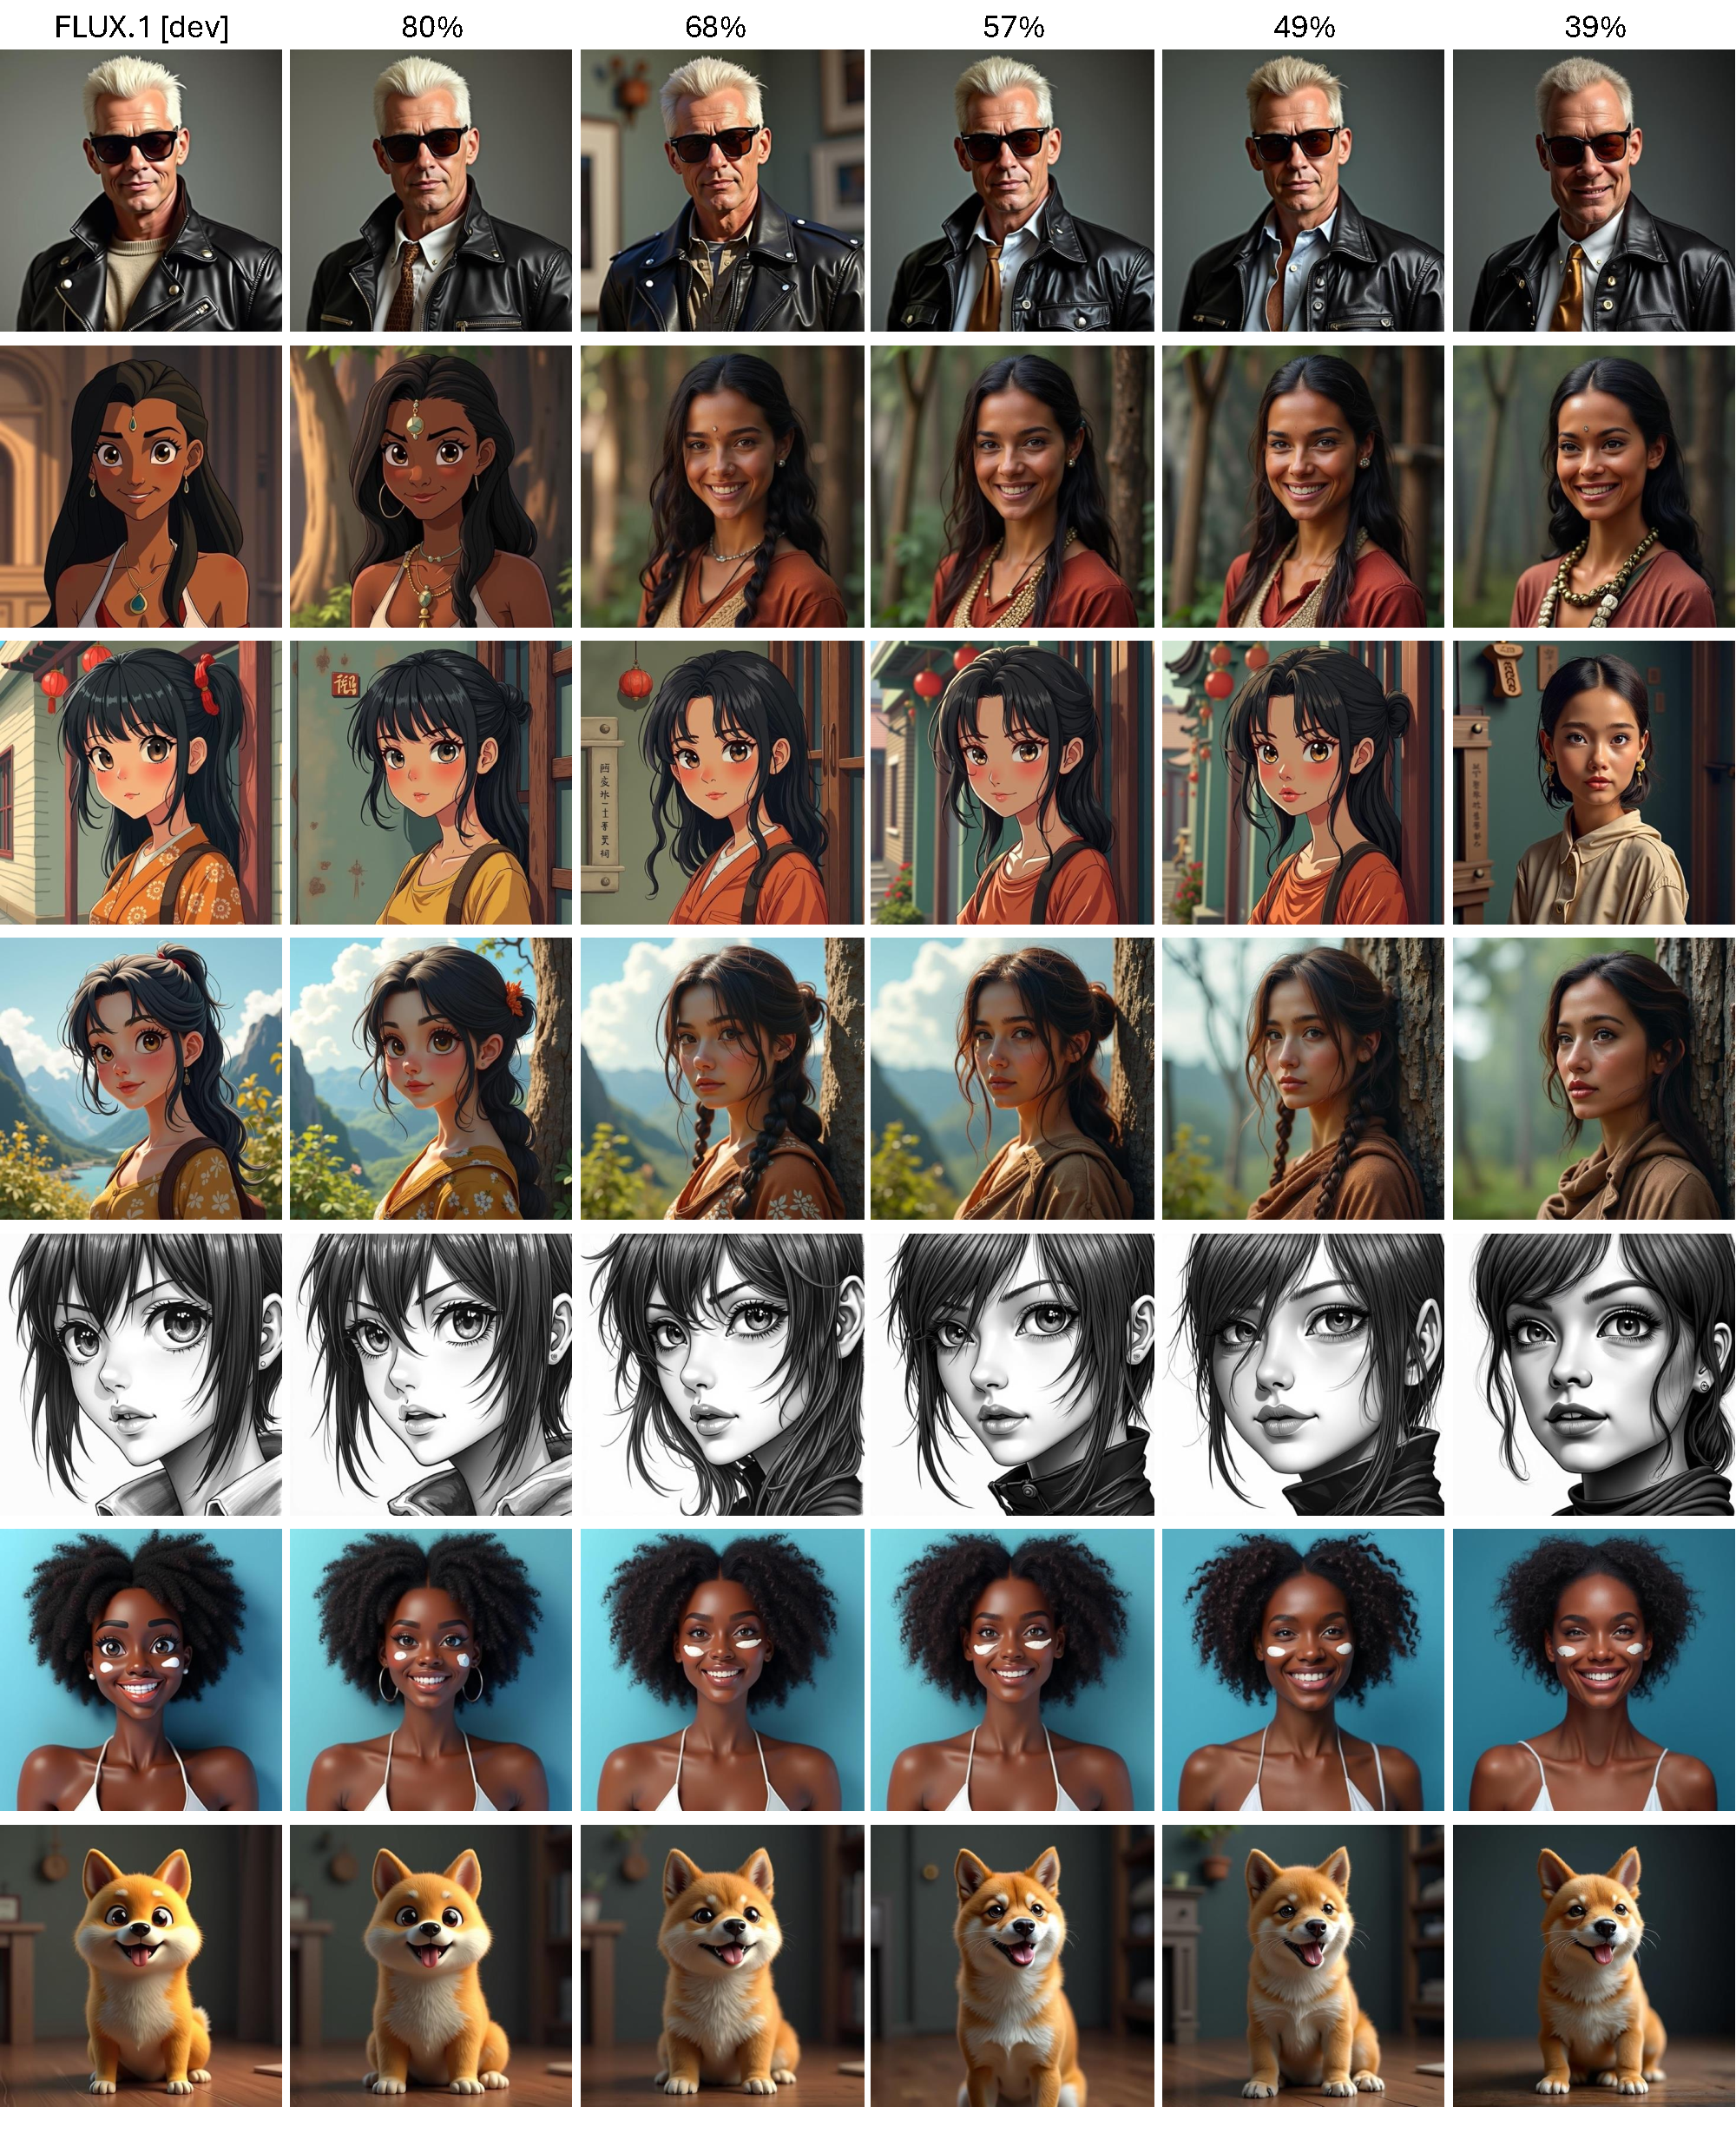
\includegraphics[width=\textwidth]{images/Experimente/Flux/SVDtrunc/Appendix_DomainShift.pdf}
	\caption[Qualitative Examples: Domain Shift in SVDtrunc - Appendix]{Qualitative comparison of example images generated at varying compression ratios using SVDtrunc, illustrating the gradual domain-shift observed with increasing compression levels.}
	\label{fig:SVDtruncFlux_ShiftAppx}
\end{figure}

	\begin{figure}[H]
	\centering
	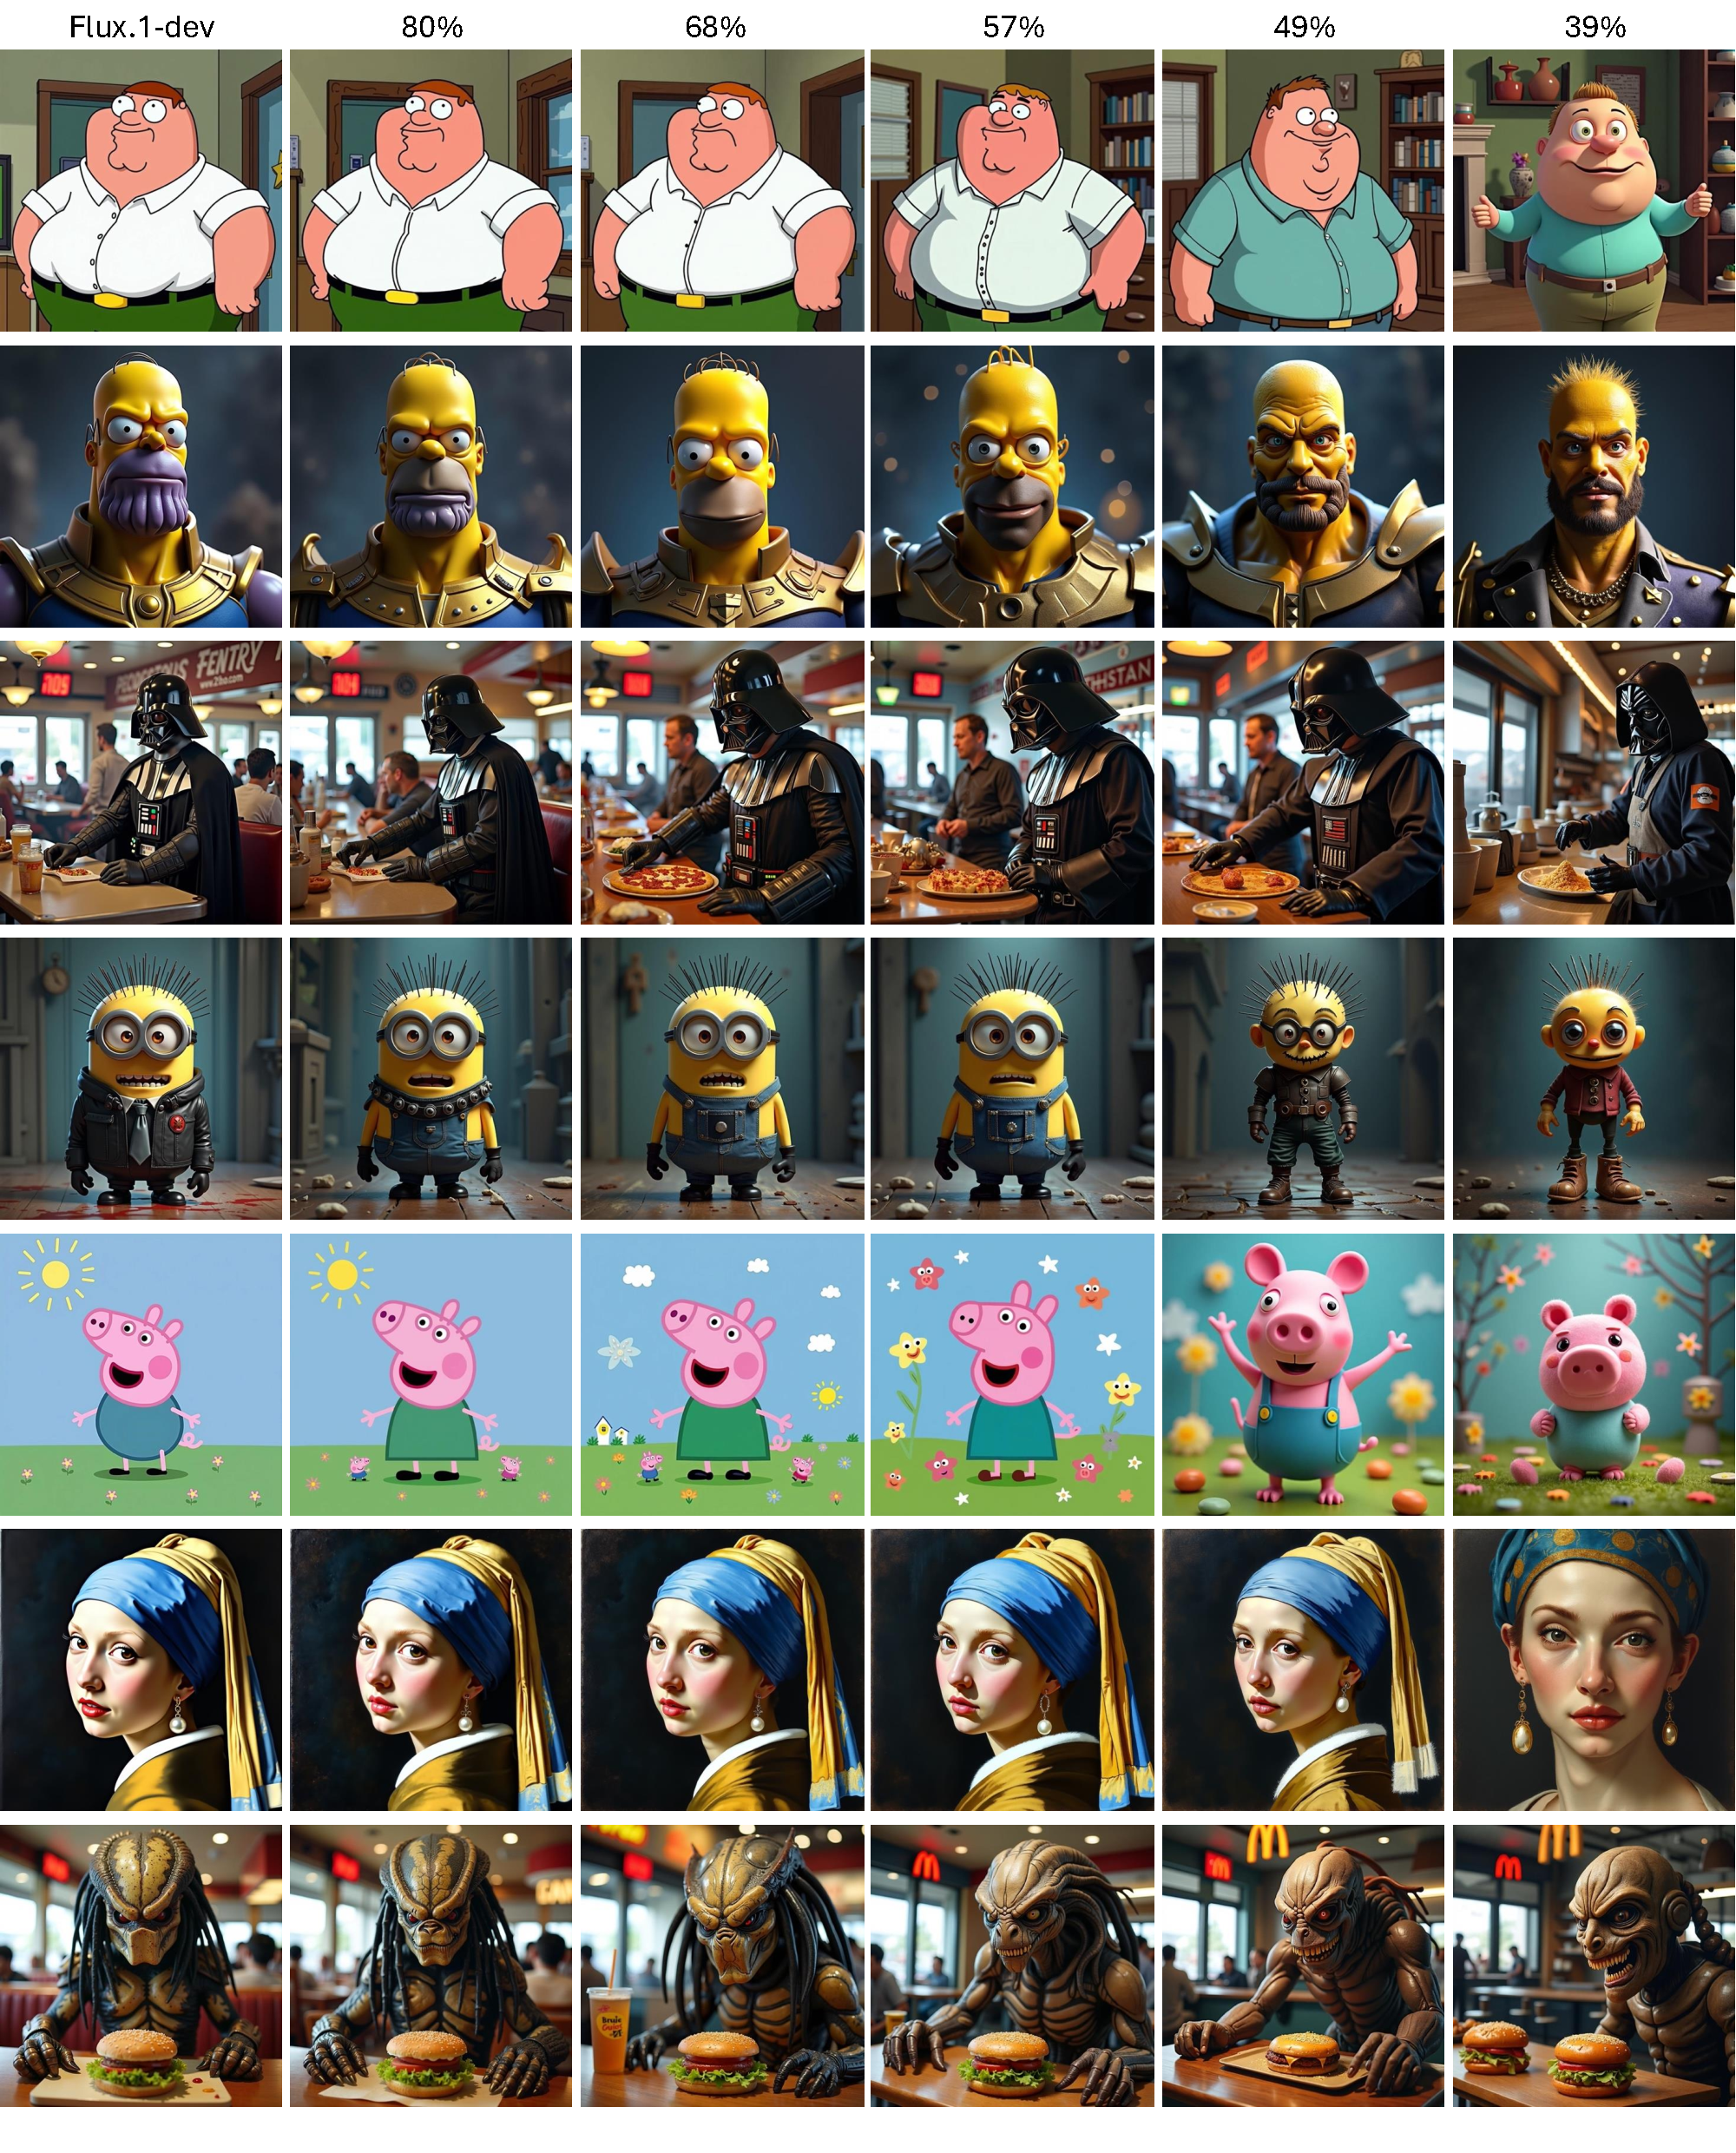
\includegraphics[width=\textwidth]{images/Experimente/Flux/SVDtrunc/Appendix_MemorizationLoss.pdf}
	\caption[Qualitative Examples: Memorization Loss in SVDtrunc - Appendix]{Qualitative comparison of example images generated at varying compression ratios using SVDtrunc, illustrating the gradual memorization-loss observed with increasing compression levels.}
	\label{fig:SVDtrunc_Memorization_Loss_Appx}
\end{figure}


\section{GRASP}
The block importance ranking from \cite{FastFlux}, which was used in Sec \ref{sec:GRASPForDiTs}, is shown in Fig. \ref{fig:GRAPSImportanceRanking}. Tab. \ref{tab:GRASPSVD_ranks} specifies the exact ranks used for the \gls{SVD} compression of the individual matrices of the double-stream blocks, and Tab. \ref{tab:GRASPpruned_blocks} lists the exact blocks that were compressed.
\subsubsection{Block Importance Ranking}
\label{app:GRASP_BlockImportance}
For this experiment the importance of blocks determined in \cite{FastFlux} was leveraged. Below the figure from the corresponding work is presented. 

\begin{figure}[htbp]
	\centering
	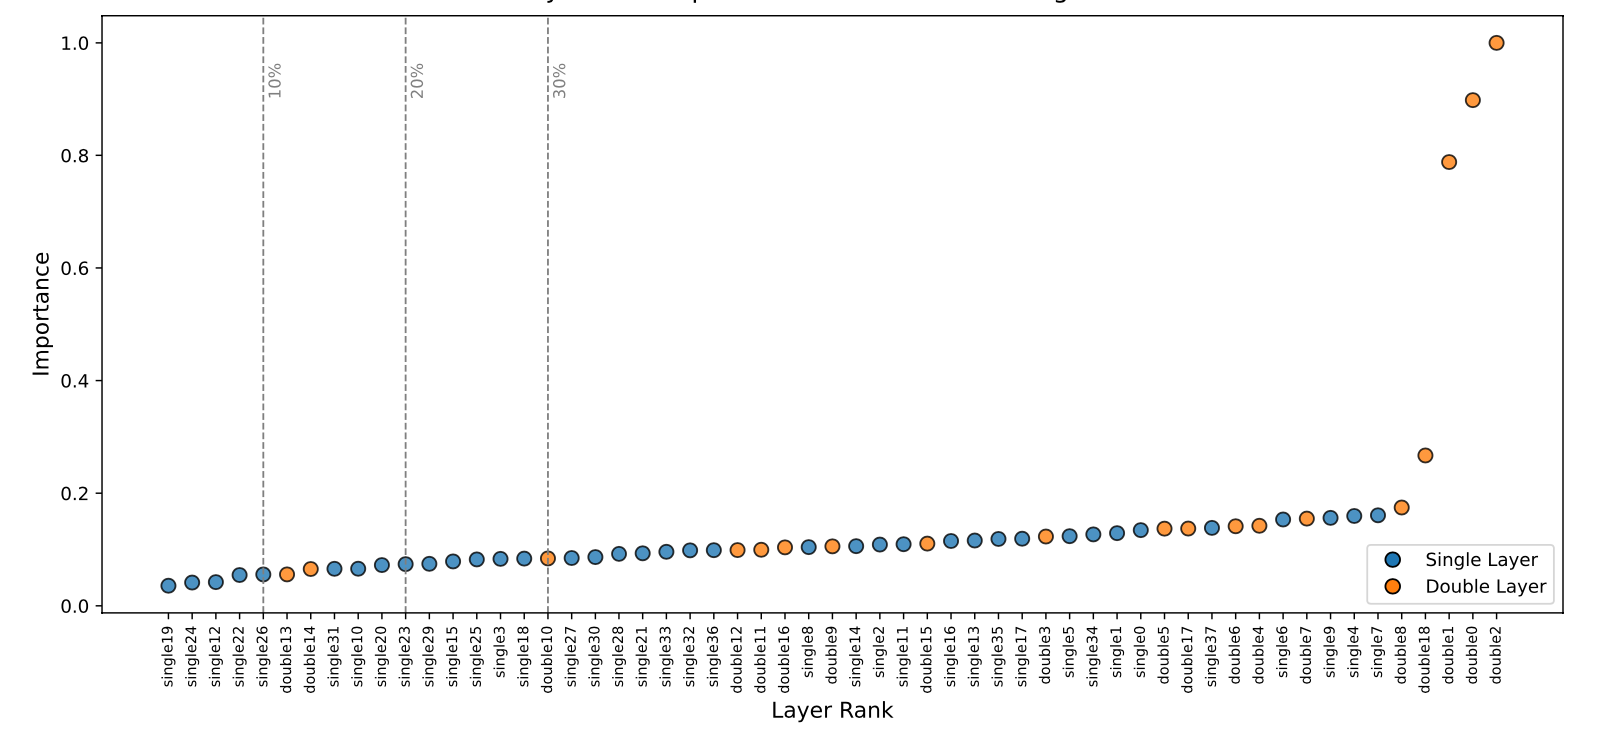
\includegraphics[width=0.9\textwidth]{images/Experimente/Flux/Training_Free/BlockImportanceFastFlux.png}
	\caption[Training-Free: Flux.1-dev Block Importance Ranking]{Block importance for Flux.1-dev taken from \cite{FastFlux}.}
	\label{fig:GRAPSImportanceRanking}
\end{figure}

\subsubsection{Compression Details}
\begin{table}[h]
	
	\centering
	\caption[GRASP: \gls{SVD} Ranks]{Overview of compressed double-stream block components and the respecive rank used in \gls{GRASP}.}
	\label{tab:GRASPSVD_ranks}
	\begin{tabular}{l|c}
		\hline
		\textbf{Components Double Block} & \textbf{Rank for \gls{SVD}} \\ \hline
		Double-Stream Image Linear Layer (Attention) & $307$ \\
		Double-Stream Image MLP                      & $491$ \\
		Double-Stream Image Modulation               & $526$ \\
		Double-Stream Text Linear Layer (Attention)  & $307$ \\
		Double-Stream Text MLP                       & $491$ \\
		Double-Stream Text Modulation                & $526$ \\ \hline
	\end{tabular}
\end{table}

\begin{table}[h]
	\centering
	\caption[GRASP: Model Compression Configuration]{Overview of compressed block configurations.}
	\label{tab:GRASPpruned_blocks}
	\begin{tabular}{l c p{6cm}}
		\toprule
		\textbf{Model Size} & \textbf{\# Pruned} & \textbf{Pruned Block IDs} \\
		\midrule
		80\% & 9 & 13, 14, 10, 12, 11, 16, 9, 15, 3 \\
		74\% & 12 &  13, 14, 10, 12, 11, 16, 9, 15, 3, 5, 17, 6 \\
		68\% & 15 & 13, 14, 10, 12, 11, 16, 9, 15, 3, 5, 17, 6, 4, 7, 8 \\
		60\% & 18 & 13, 14, 10, 12, 11, 16, 9, 15, 3, 5, 17, 6, 4, 7, 8, 18, 1, 0  \\
		\bottomrule
	\end{tabular}
\end{table}

